\chapter{GSEA and ORA plots} \label{gsea-plots}

% PD-PCx
\begin{figure}[!ht]%
    \centering
    \subfloat[\centering Enrichment map for ORA. ]{{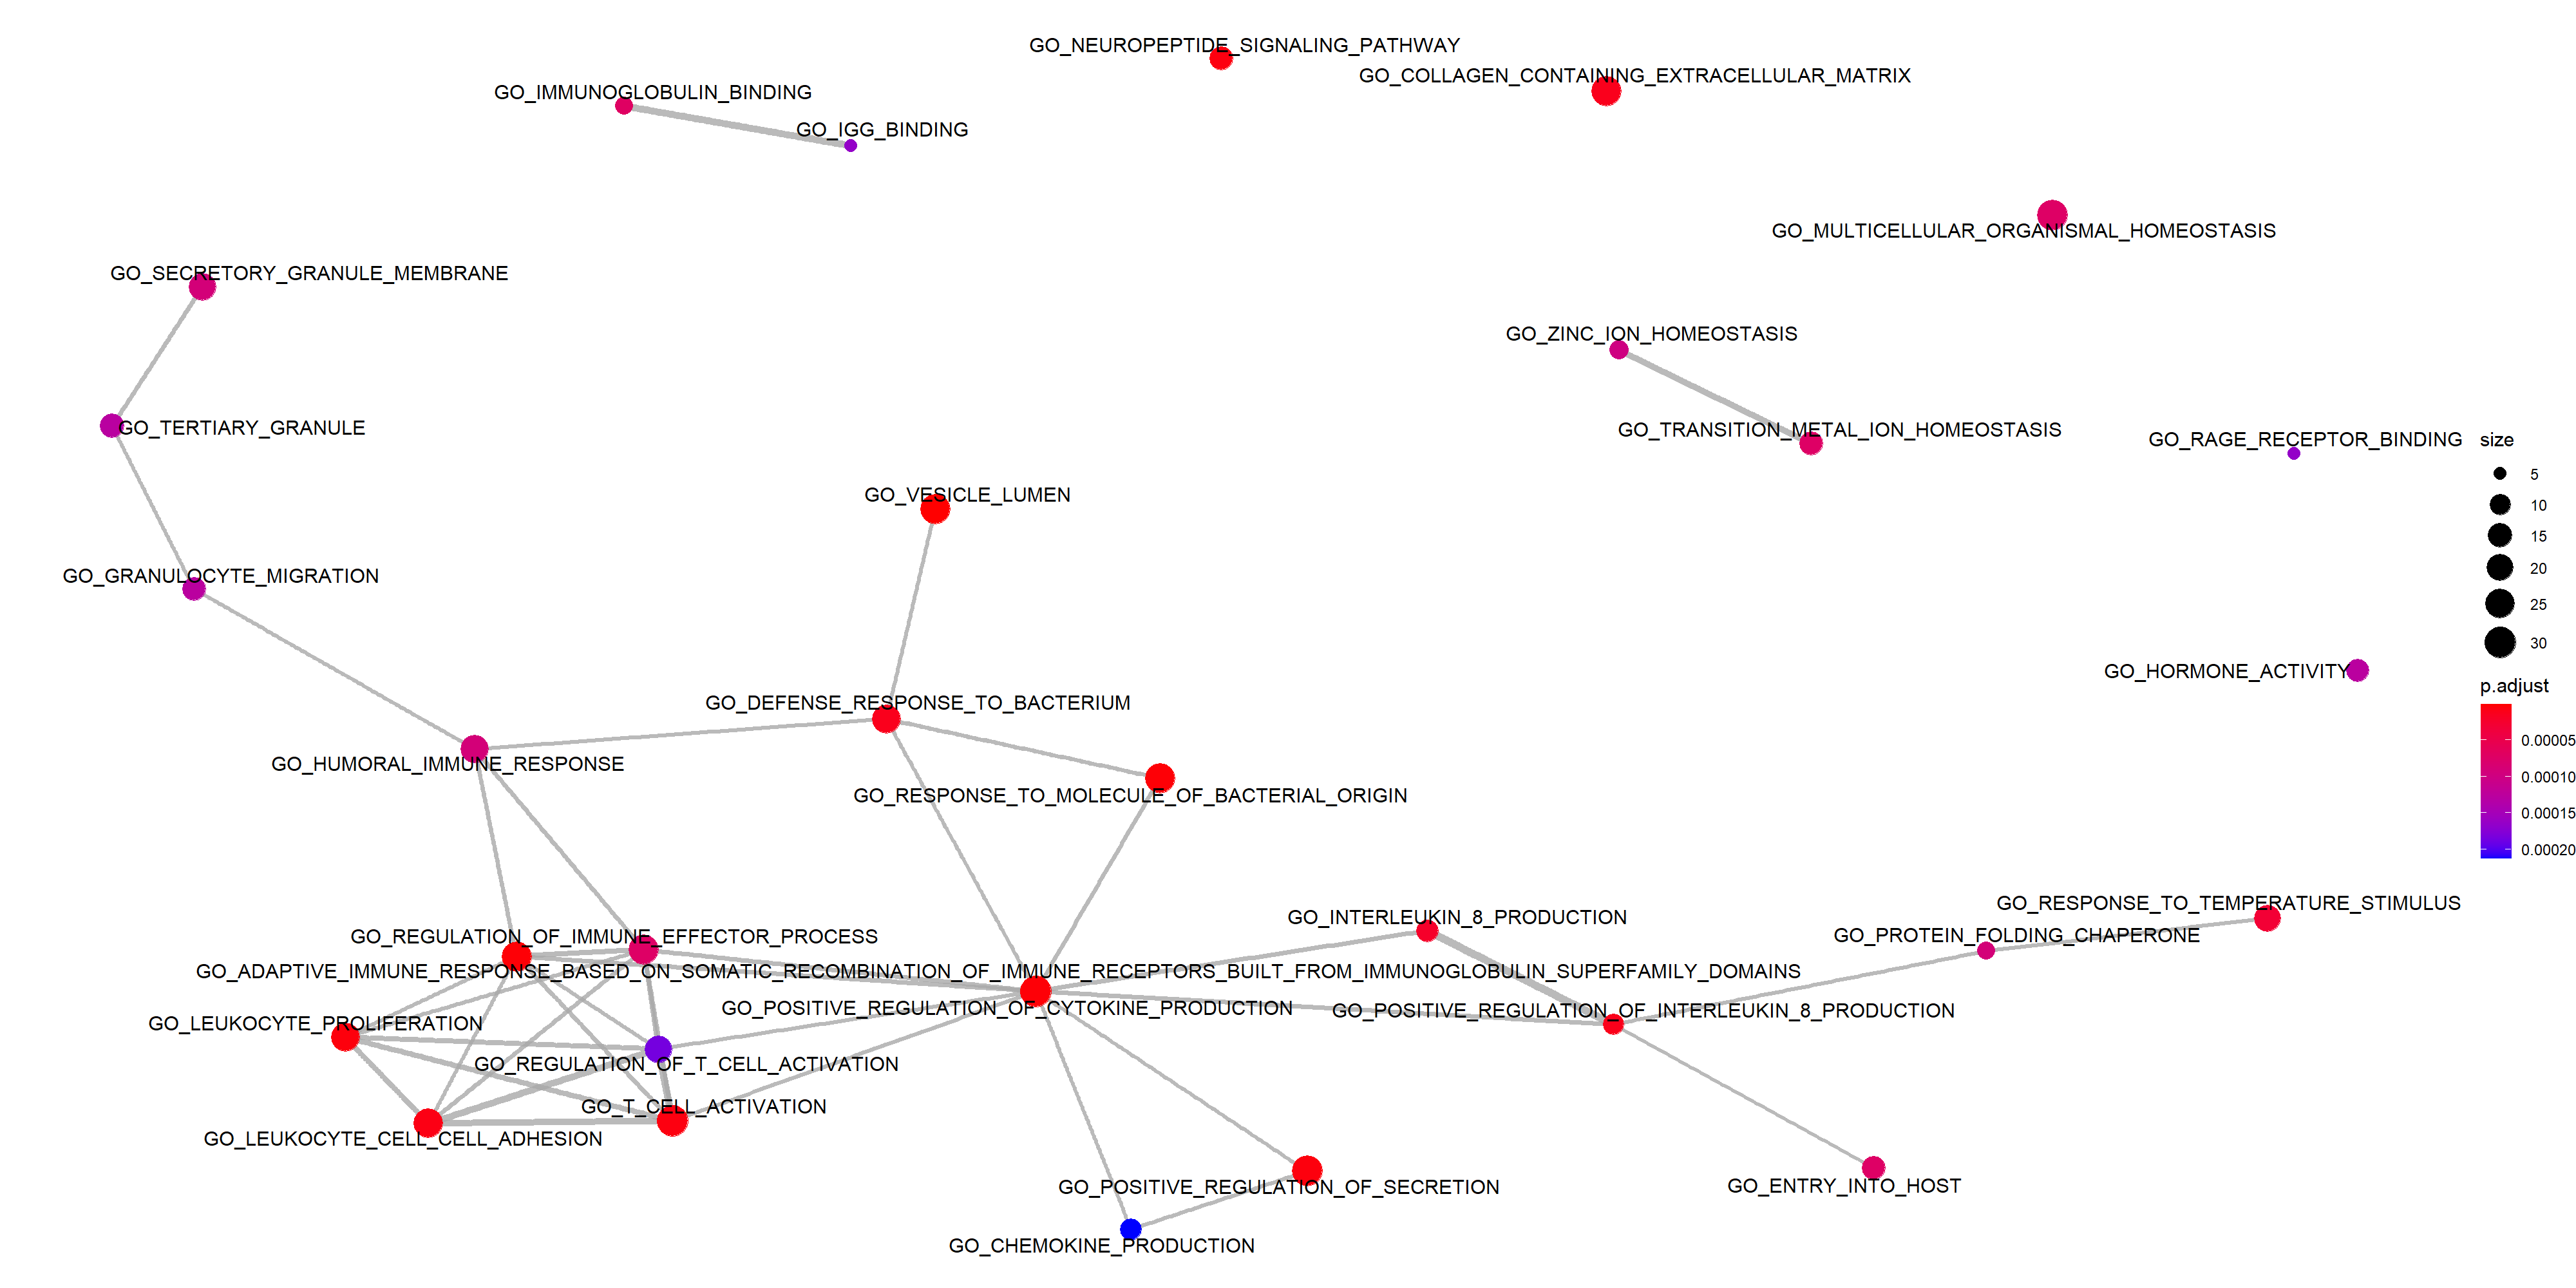
\includegraphics[width=10cm]{Figures/GSEA/CTLvsPD_emapplot.png} }}%
    \\
    \subfloat[\centering Gene-concept network for ORA. ]{{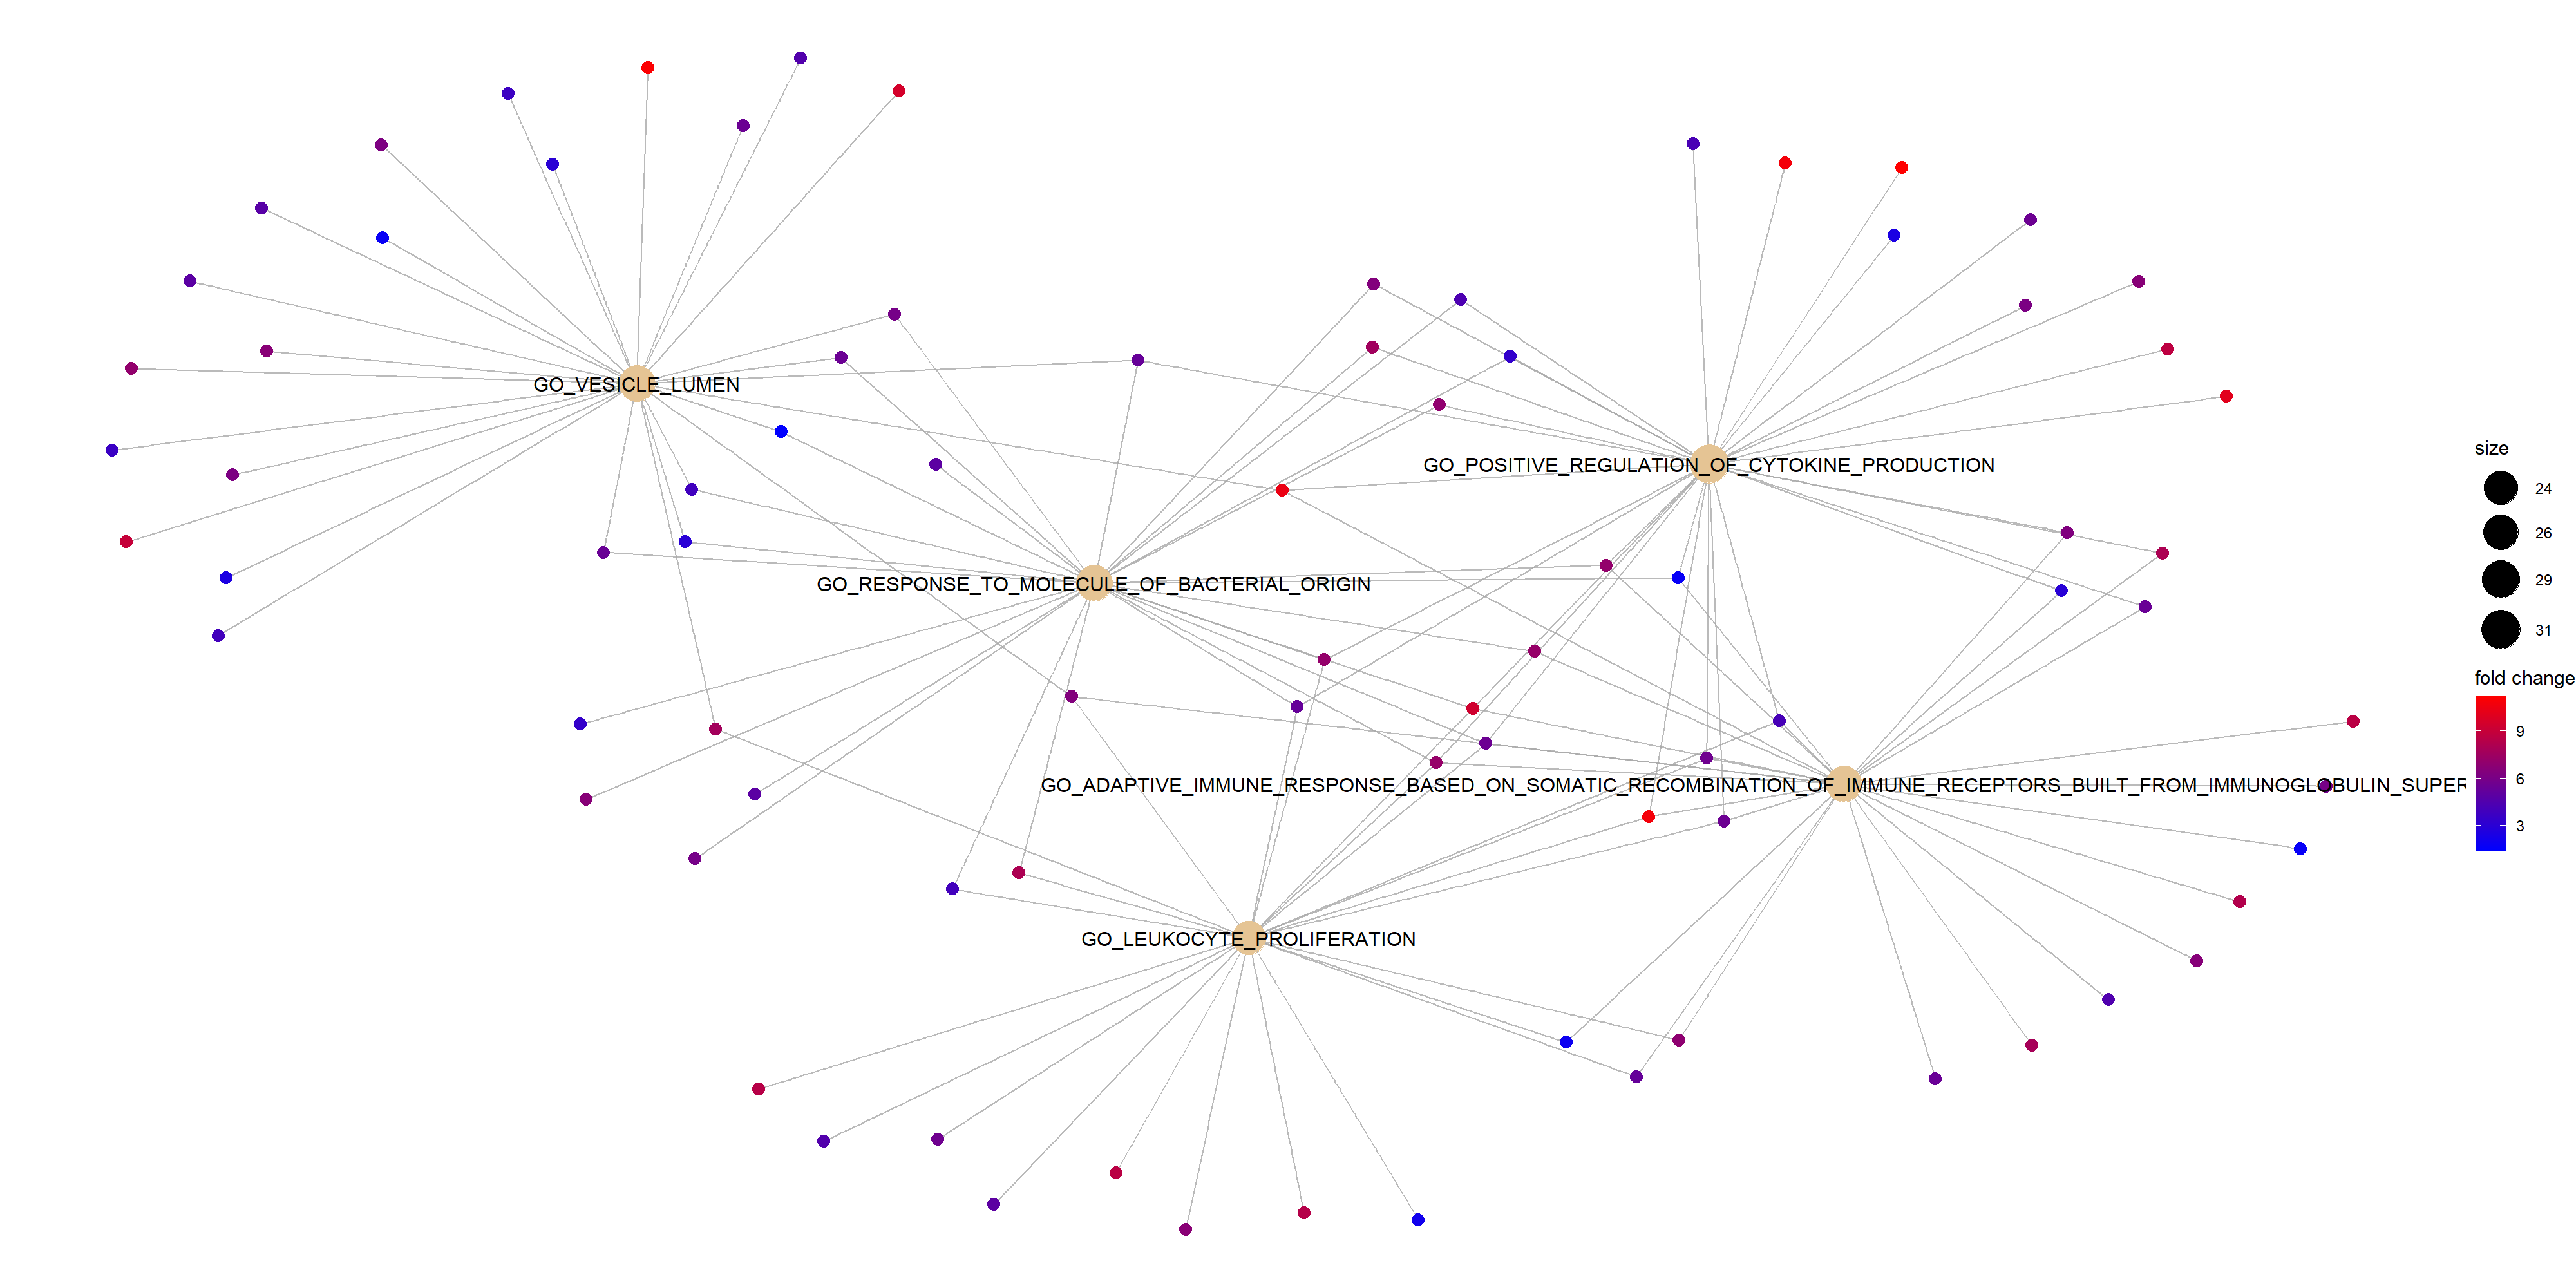
\includegraphics[width=10cm]{Figures/GSEA/CTLvsPD_cnetplot.png} }}%
    \\
    \subfloat[\centering Heatmap for ORA. ]{{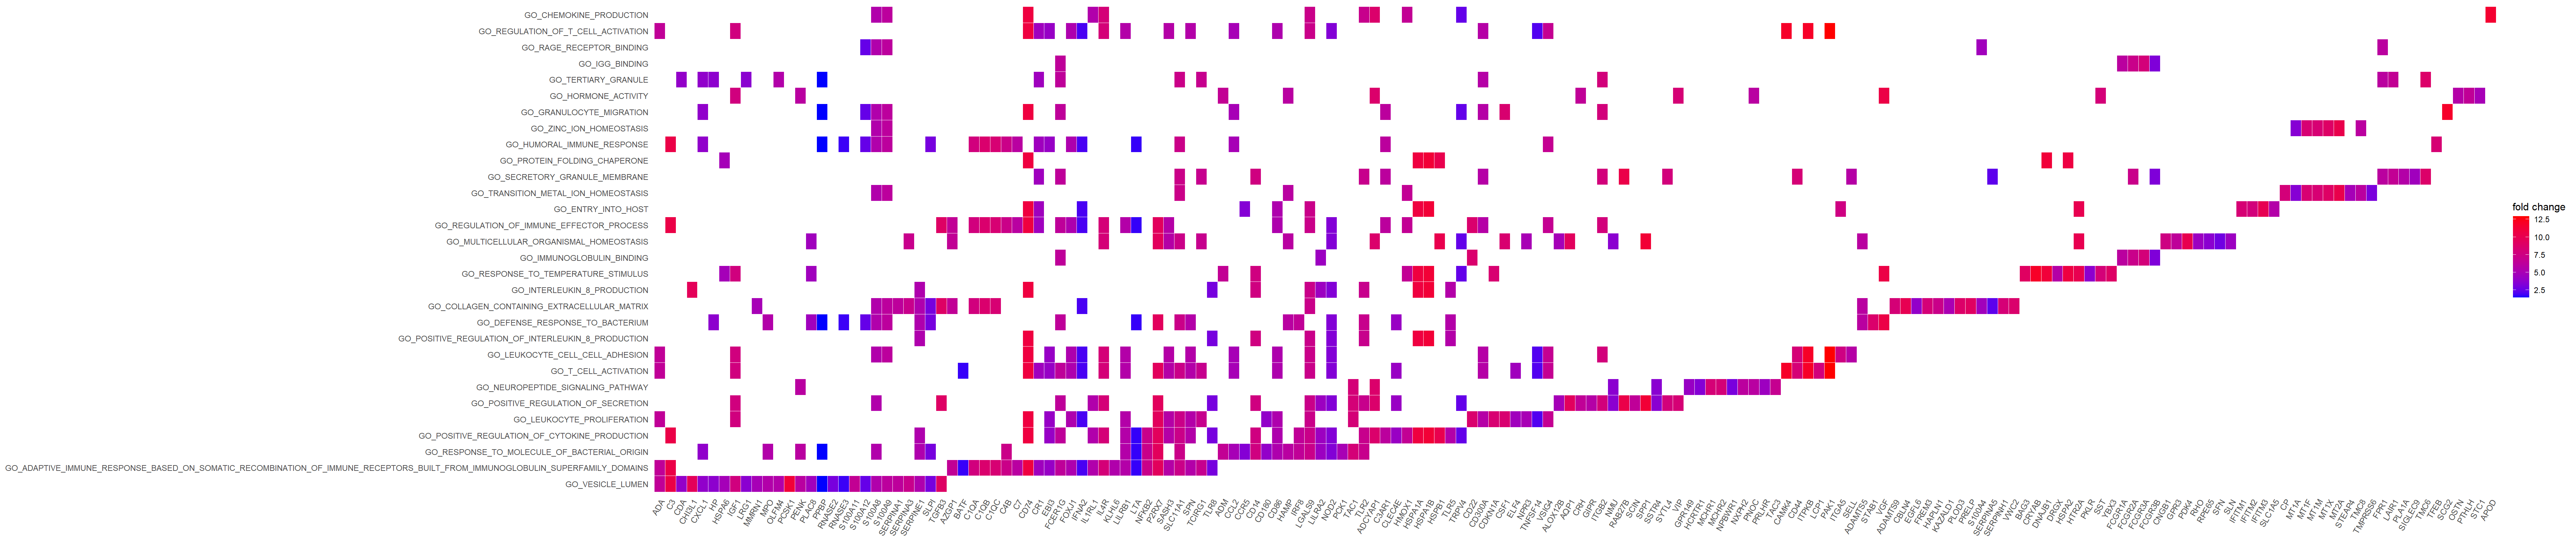
\includegraphics[width=10cm]{Figures/GSEA/CTLvsPD_heatmap.png} }}%
\caption{Functional analysis visualizations of PCx-PD.}
\end{figure}

% PD-PCx S2
\begin{figure}[!ht]%
    \centering
    \subfloat[\centering Enrichment map for ORA. ]{{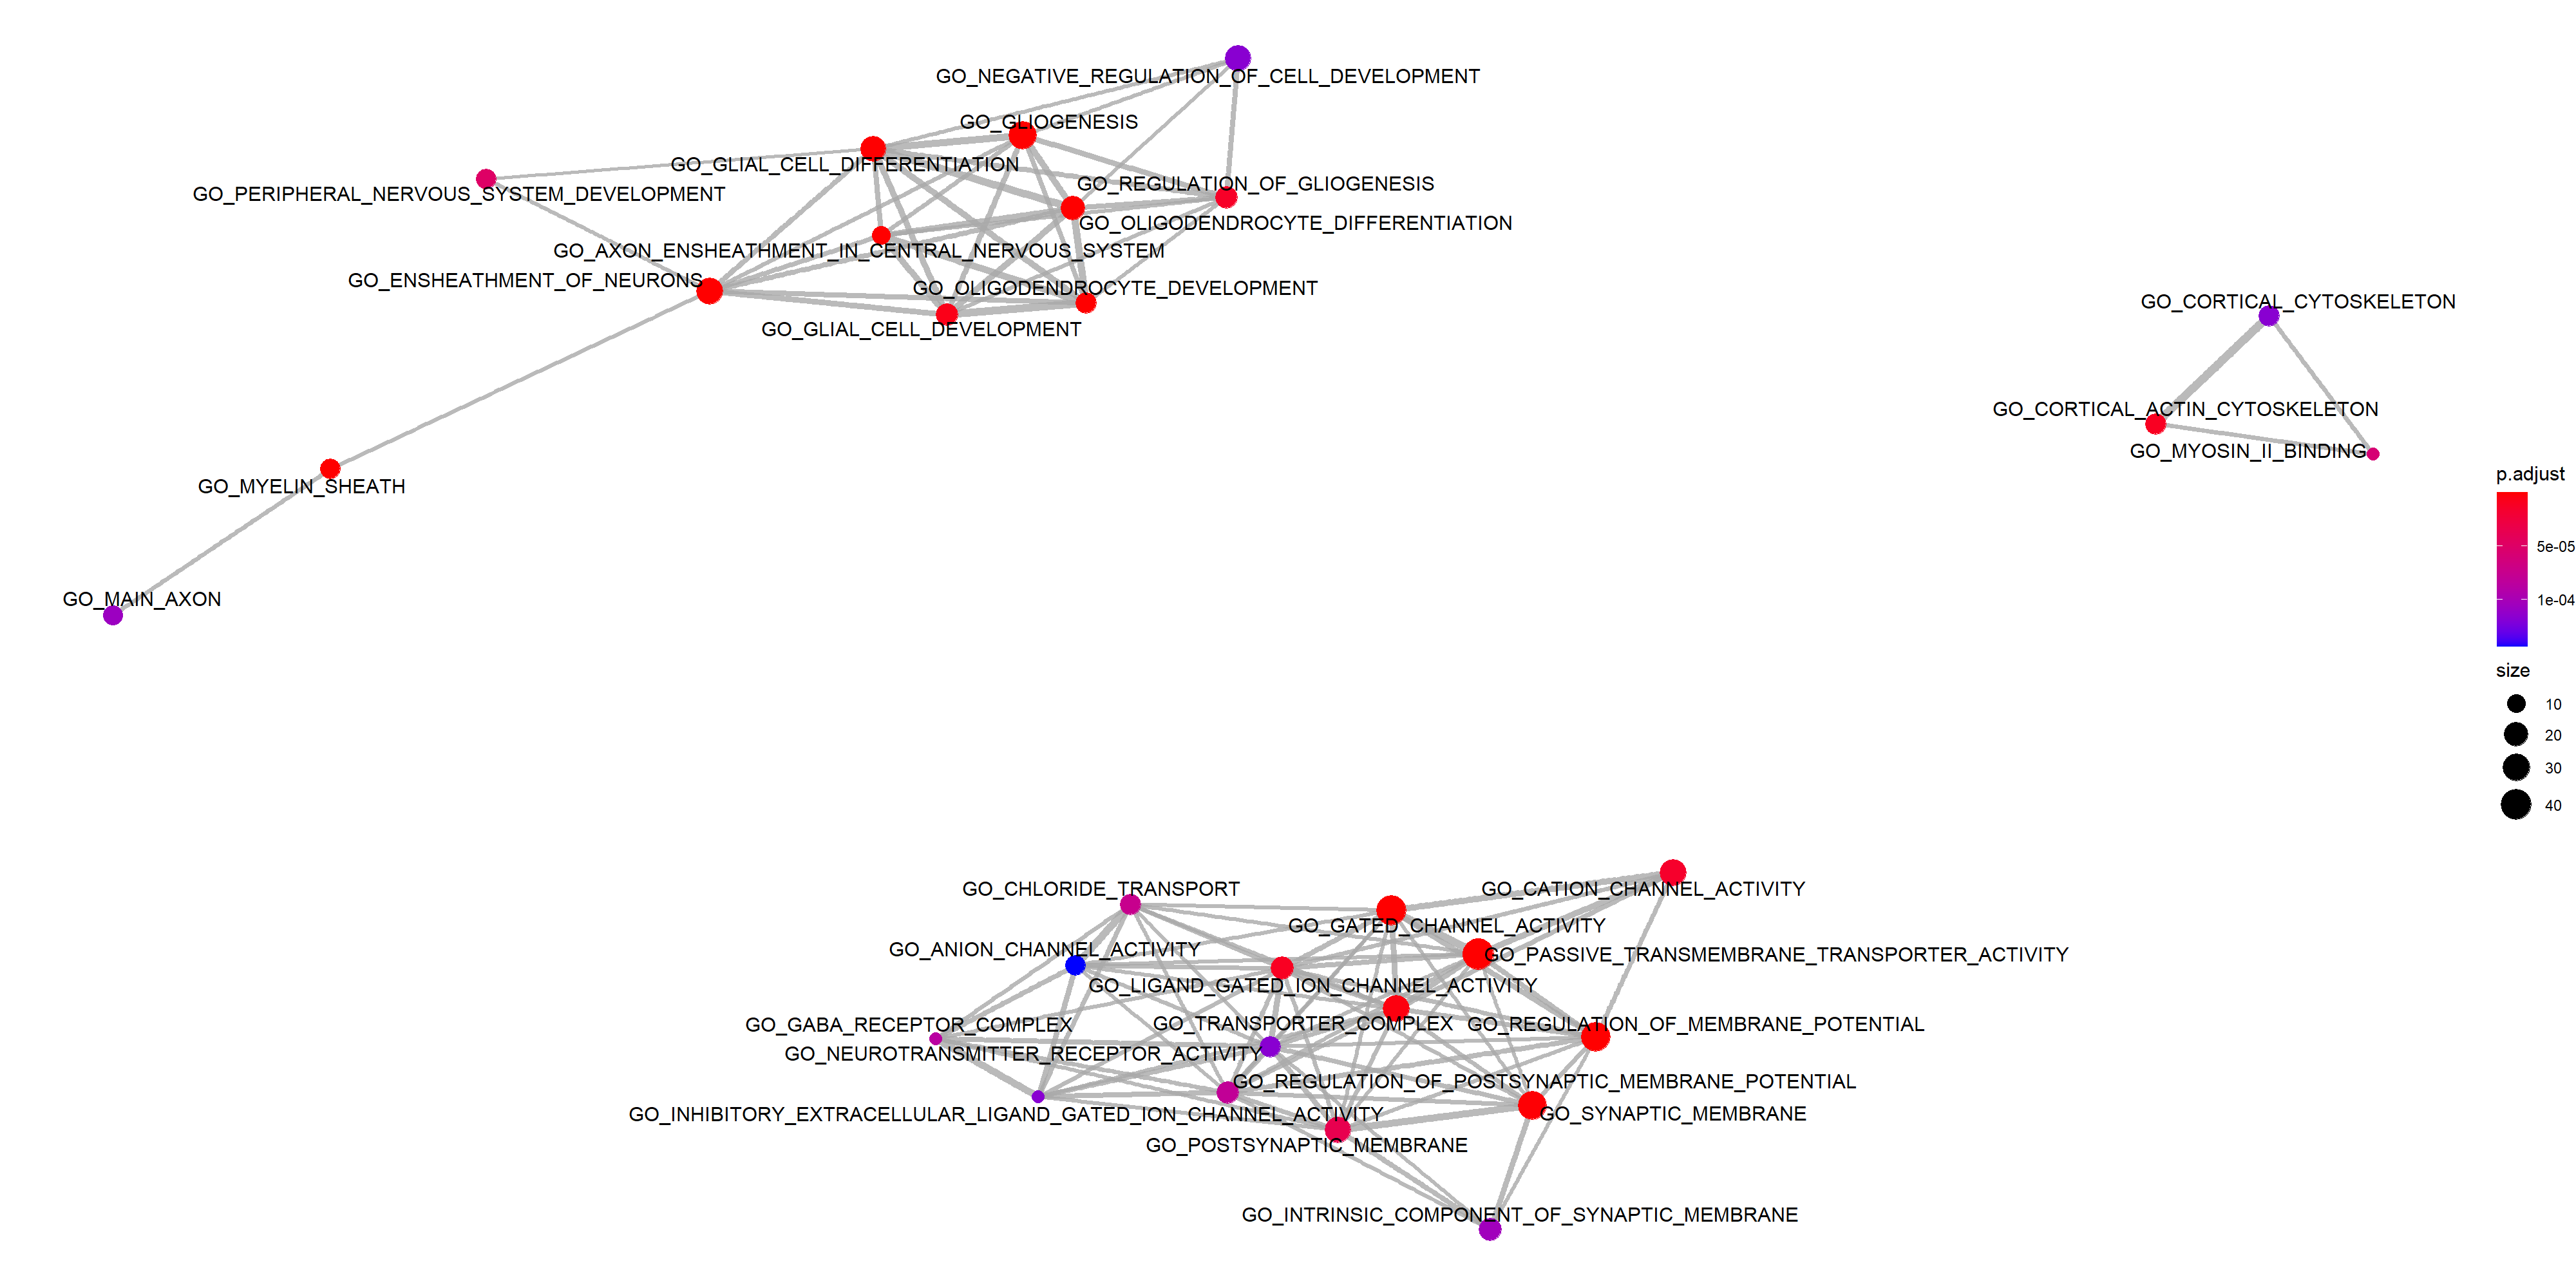
\includegraphics[width=10cm]{Figures/GSEA/CTLvs2PD_e_emapplot.png} }}%
    \\
    \subfloat[\centering Gene-concept network for ORA. ]{{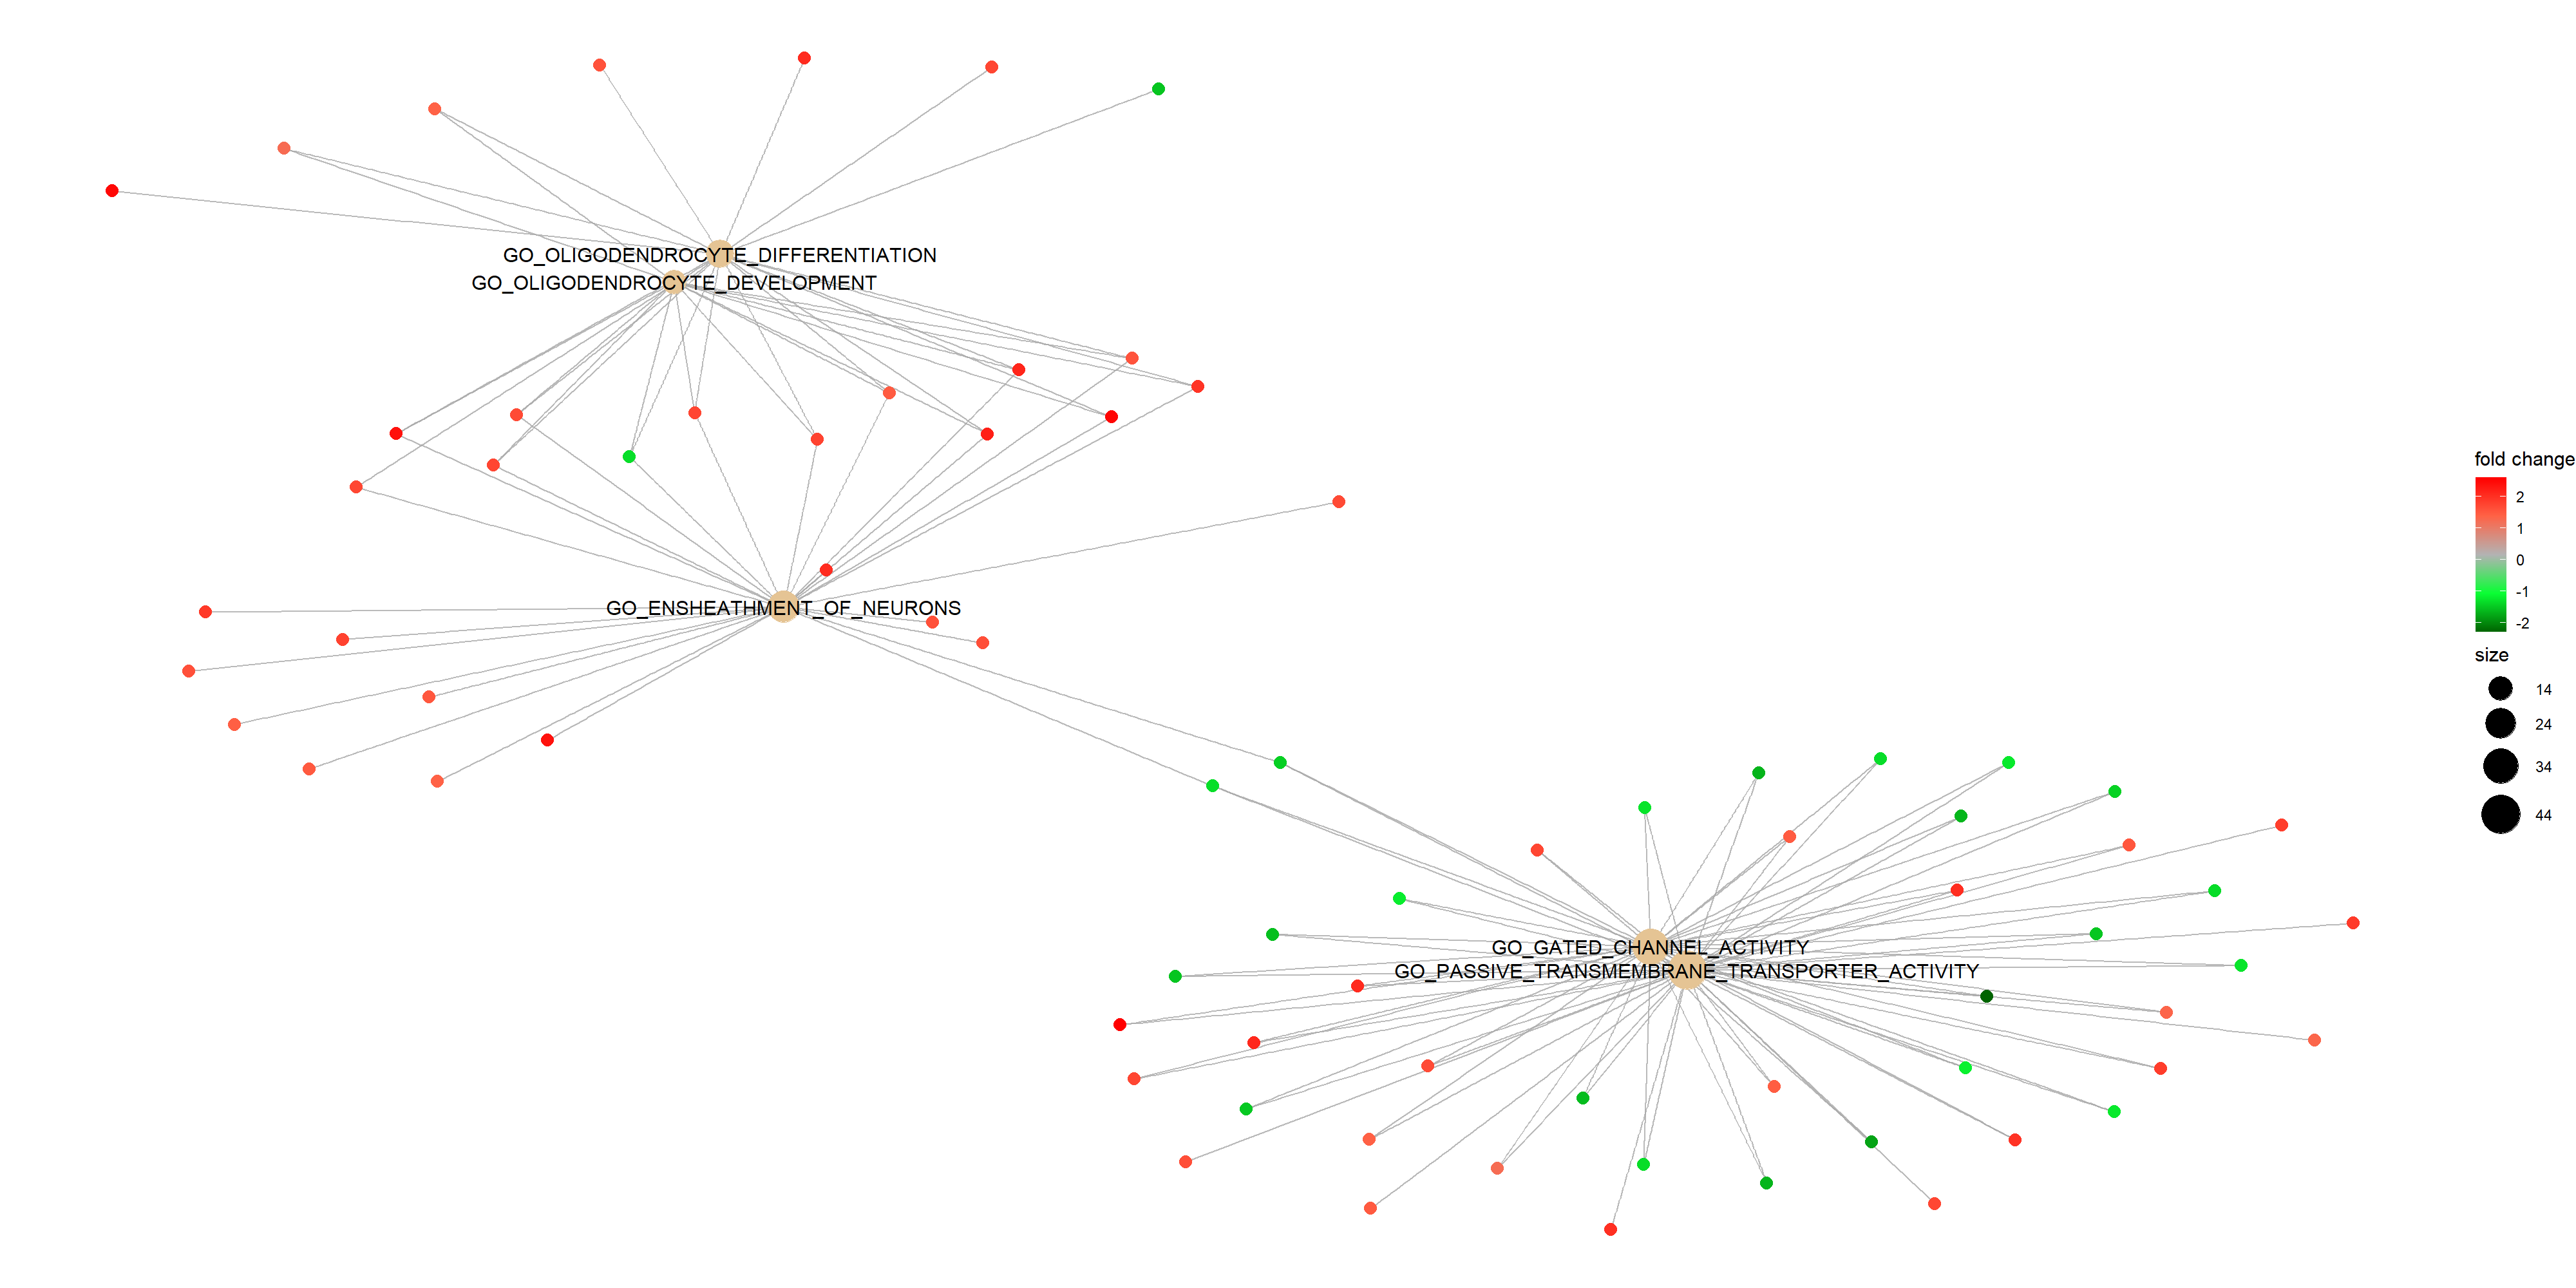
\includegraphics[width=10cm]{Figures/GSEA/CTLvs2PD_e_cnetplot.png} }}%
    \\
    \subfloat[\centering Heatmap for ORA. ]{{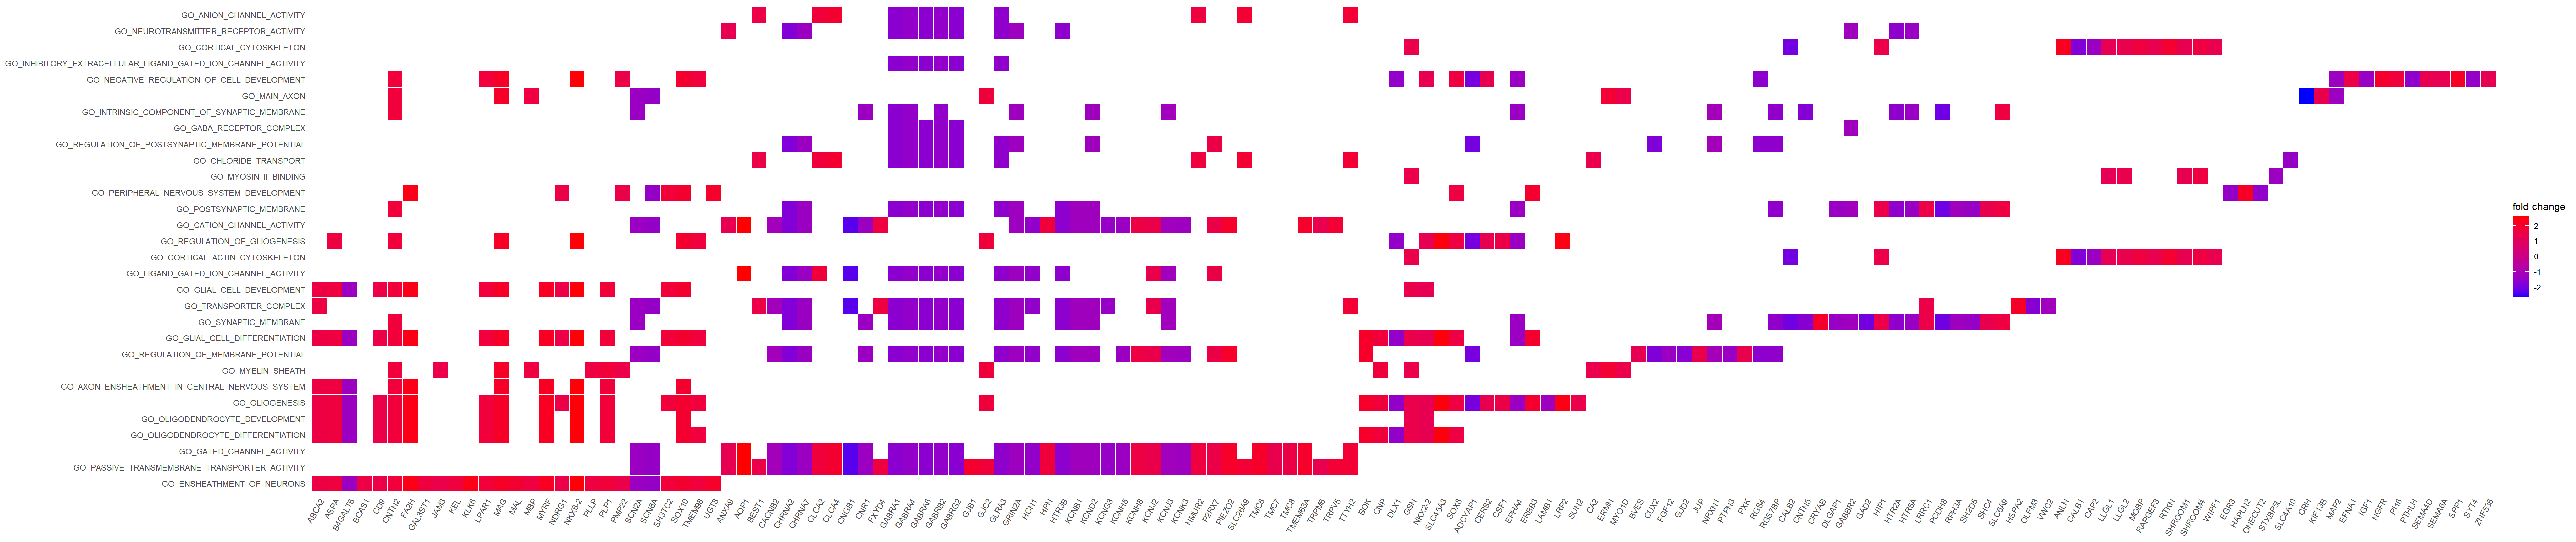
\includegraphics[width=10cm]{Figures/GSEA/CTLvs2PD_e_heatmap.png} }}%
\caption{Functional analysis visualizations of PCx-PD-S2.}
\end{figure}

% PD-PCx S3
\begin{figure}[!ht]%
    \centering
    \subfloat[\centering Enrichment map for ORA. ]{{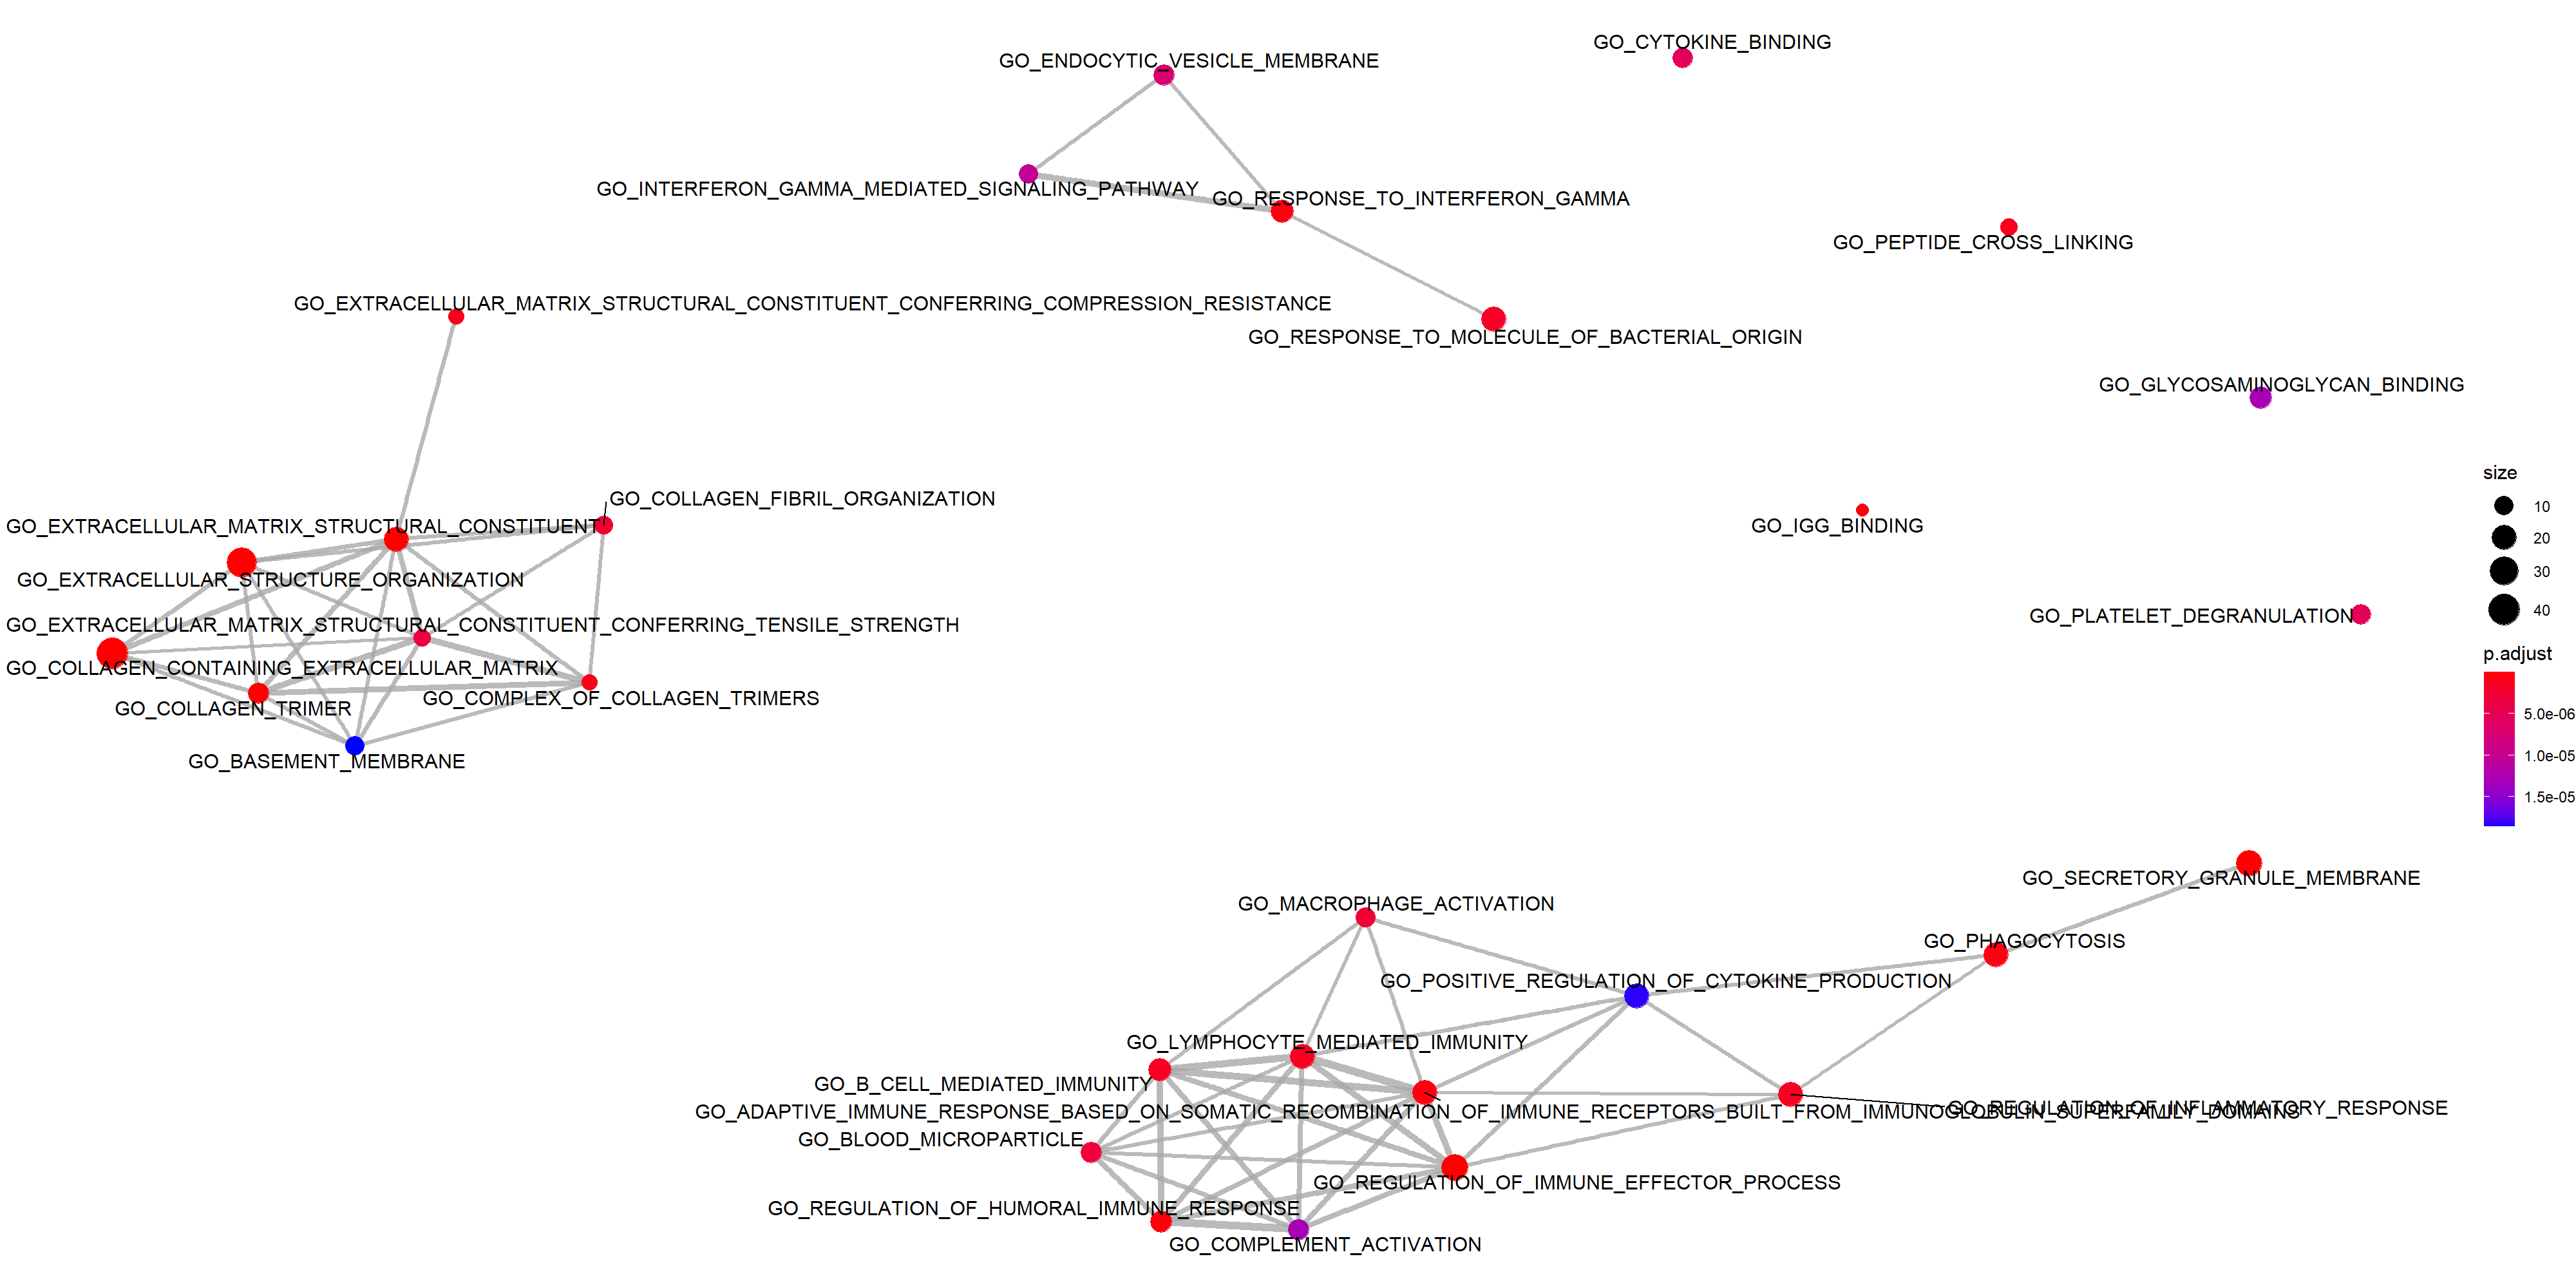
\includegraphics[width=10cm]{Figures/GSEA/CTLvs3PD_e_emapplot.png} }}%
    \\
    \subfloat[\centering Gene-concept network for ORA. ]{{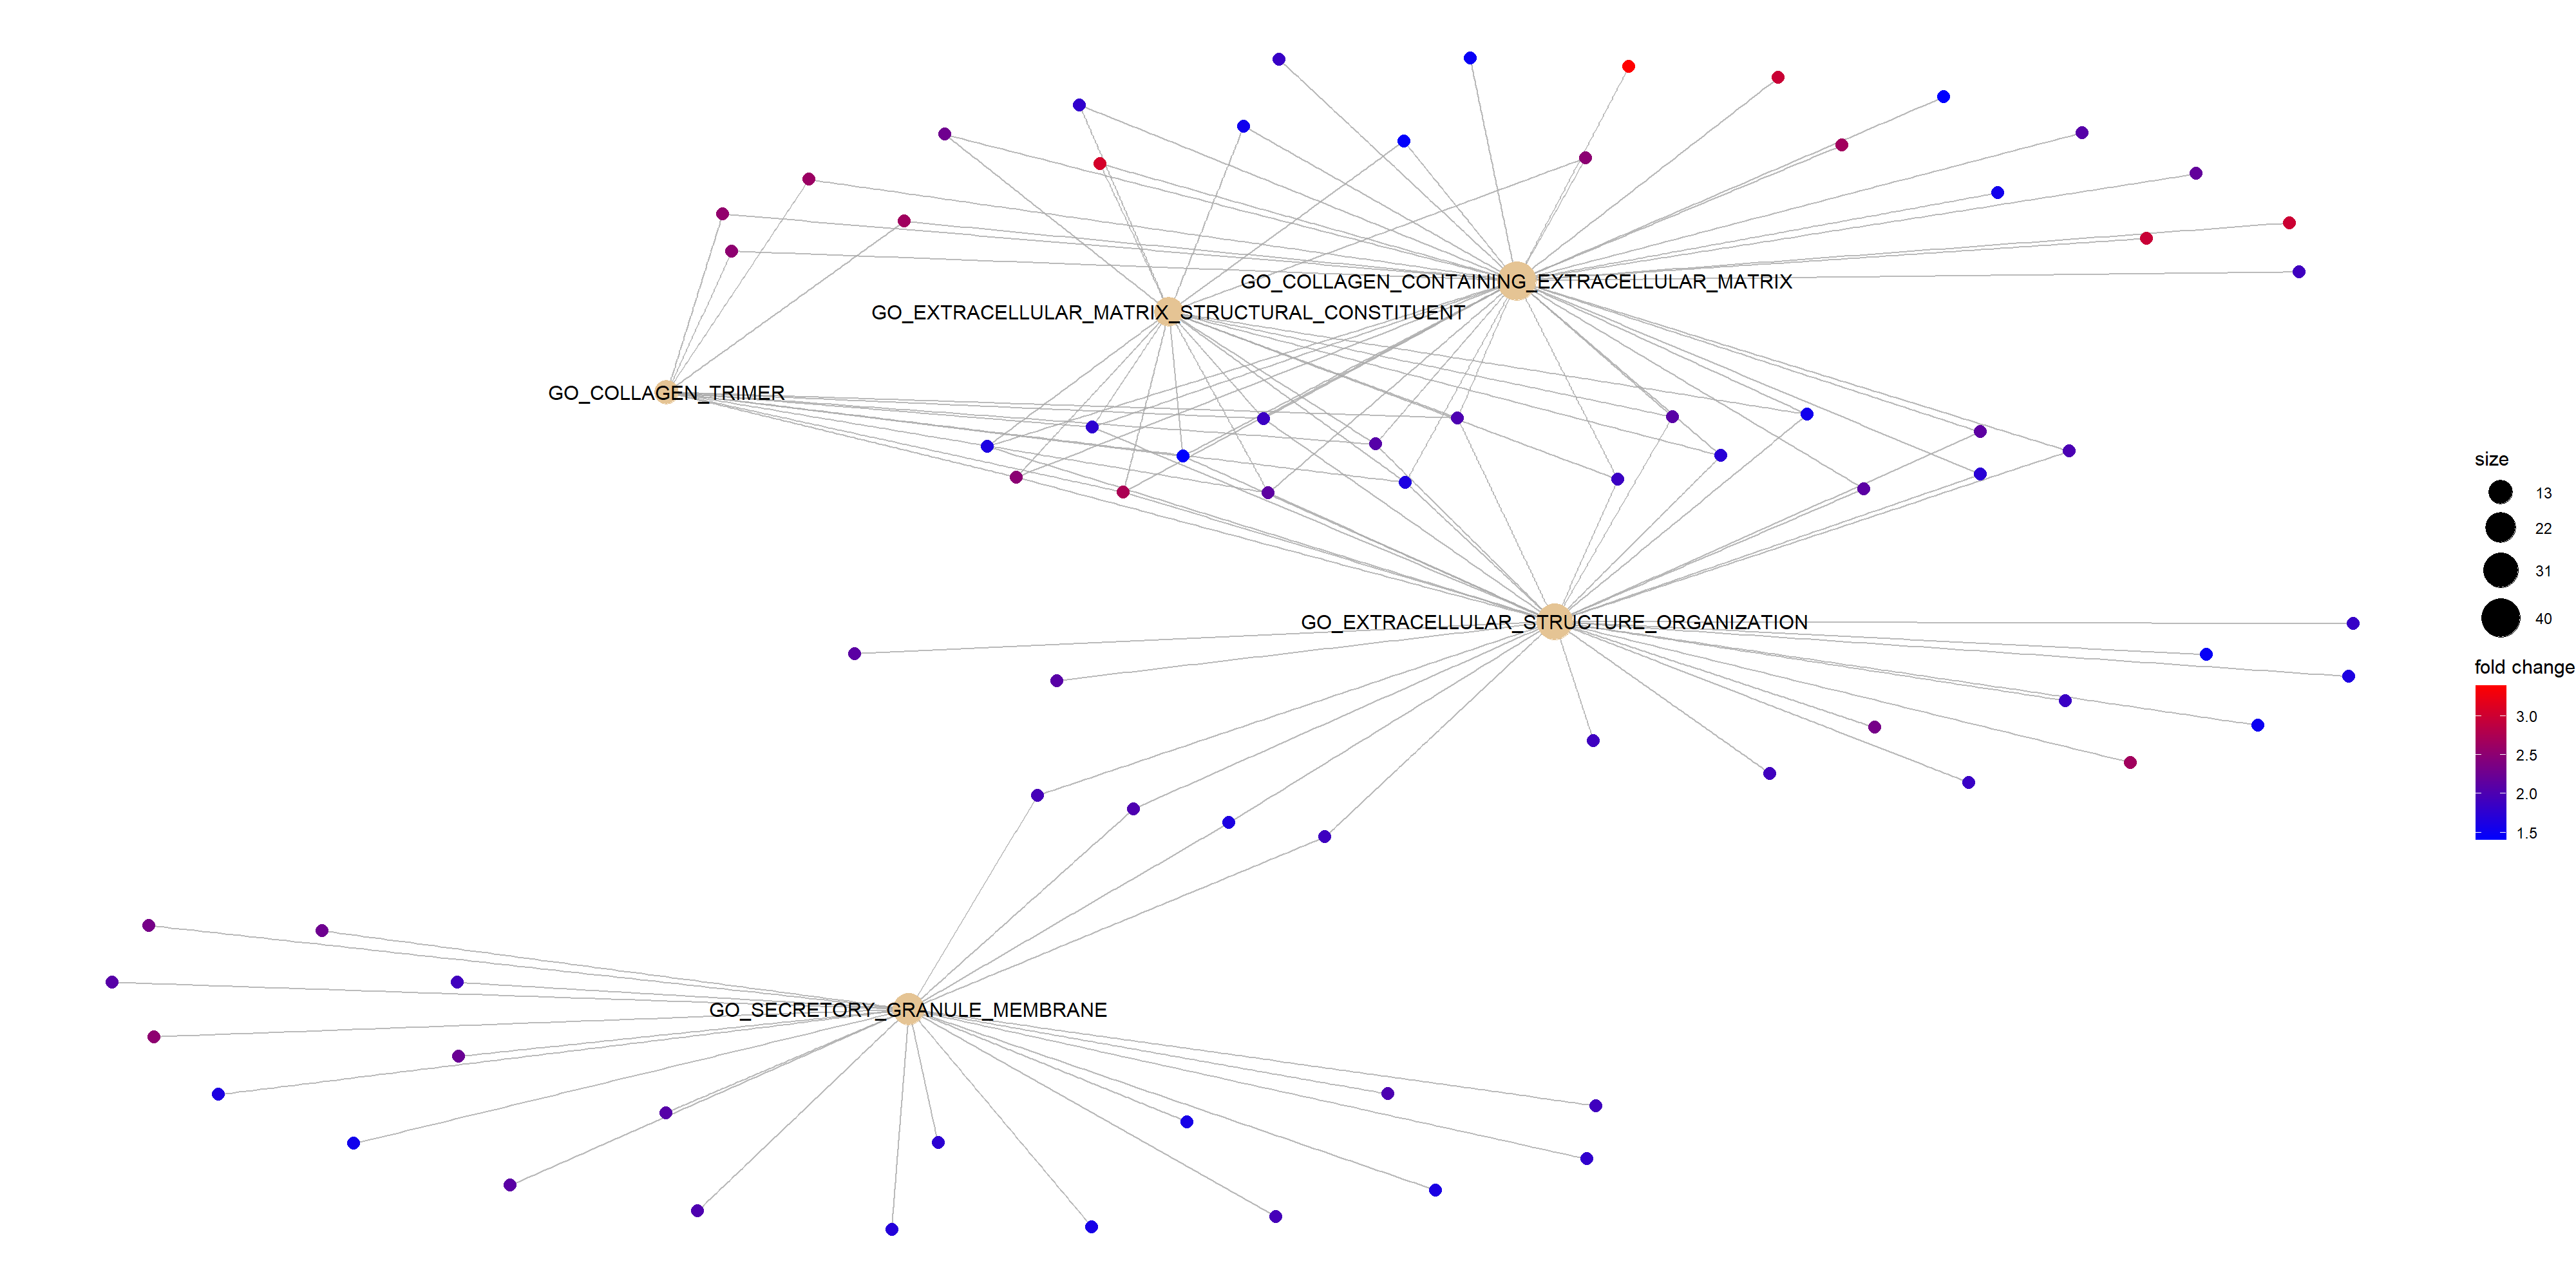
\includegraphics[width=10cm]{Figures/GSEA/CTLvs3PD_e_cnetplot.png} }}%
    \\
    \subfloat[\centering Heatmap for ORA. ]{{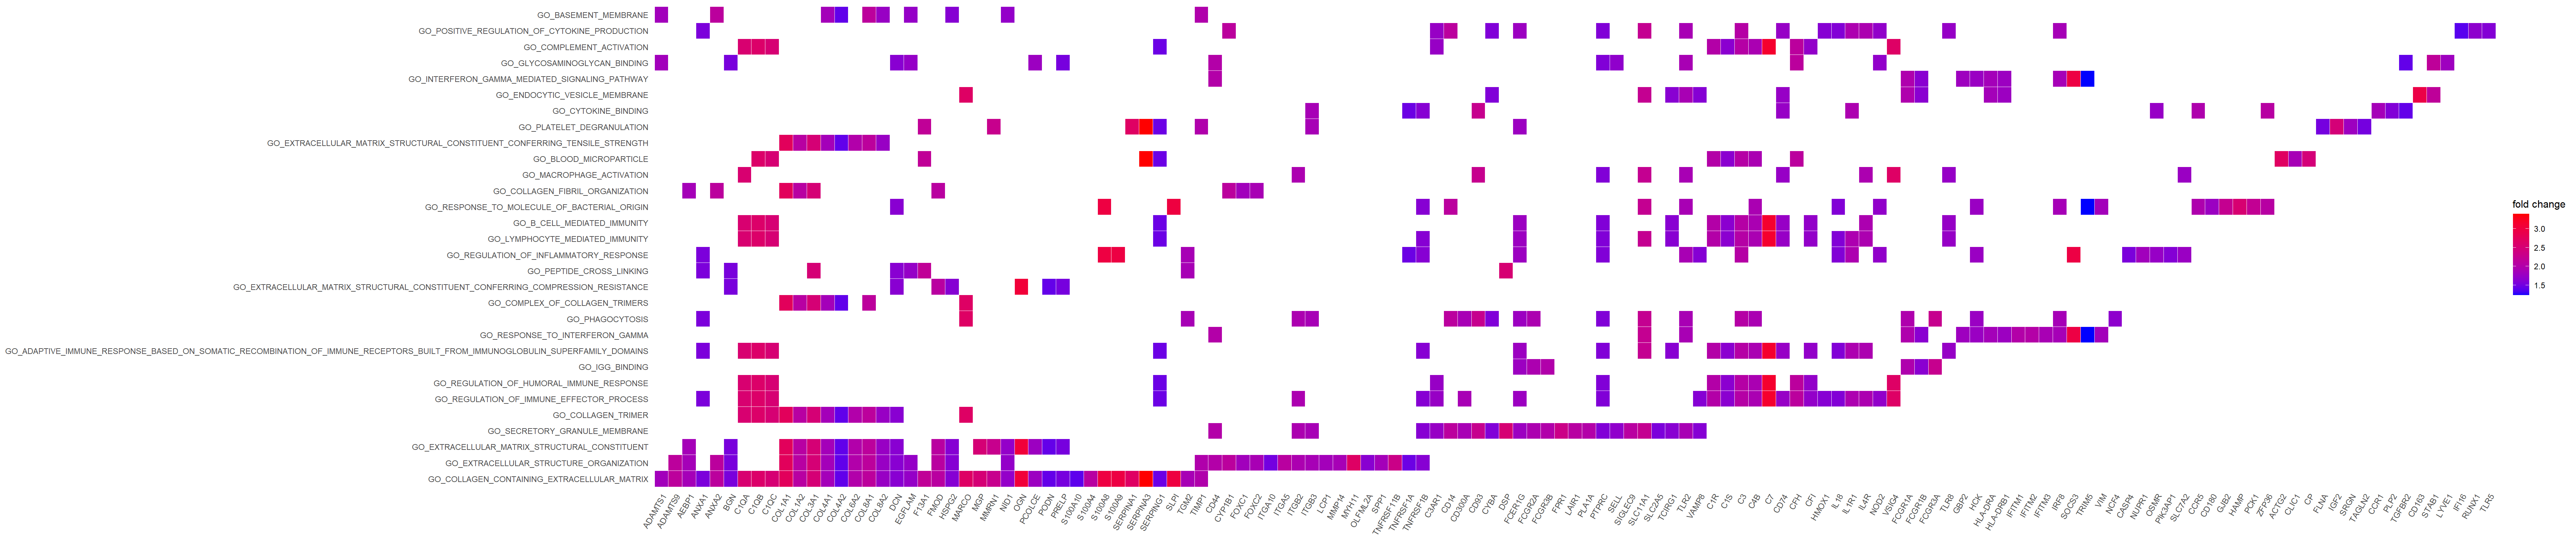
\includegraphics[width=10cm]{Figures/GSEA/CTLvs3PD_e_heatmap.png} }}%
\caption{Functional analysis visualizations of PCx-PD-S3.}
\end{figure}

% HD-PCx
\begin{figure}[!ht]%
    \centering
    \subfloat[\centering Enrichment map for ORA. ]{{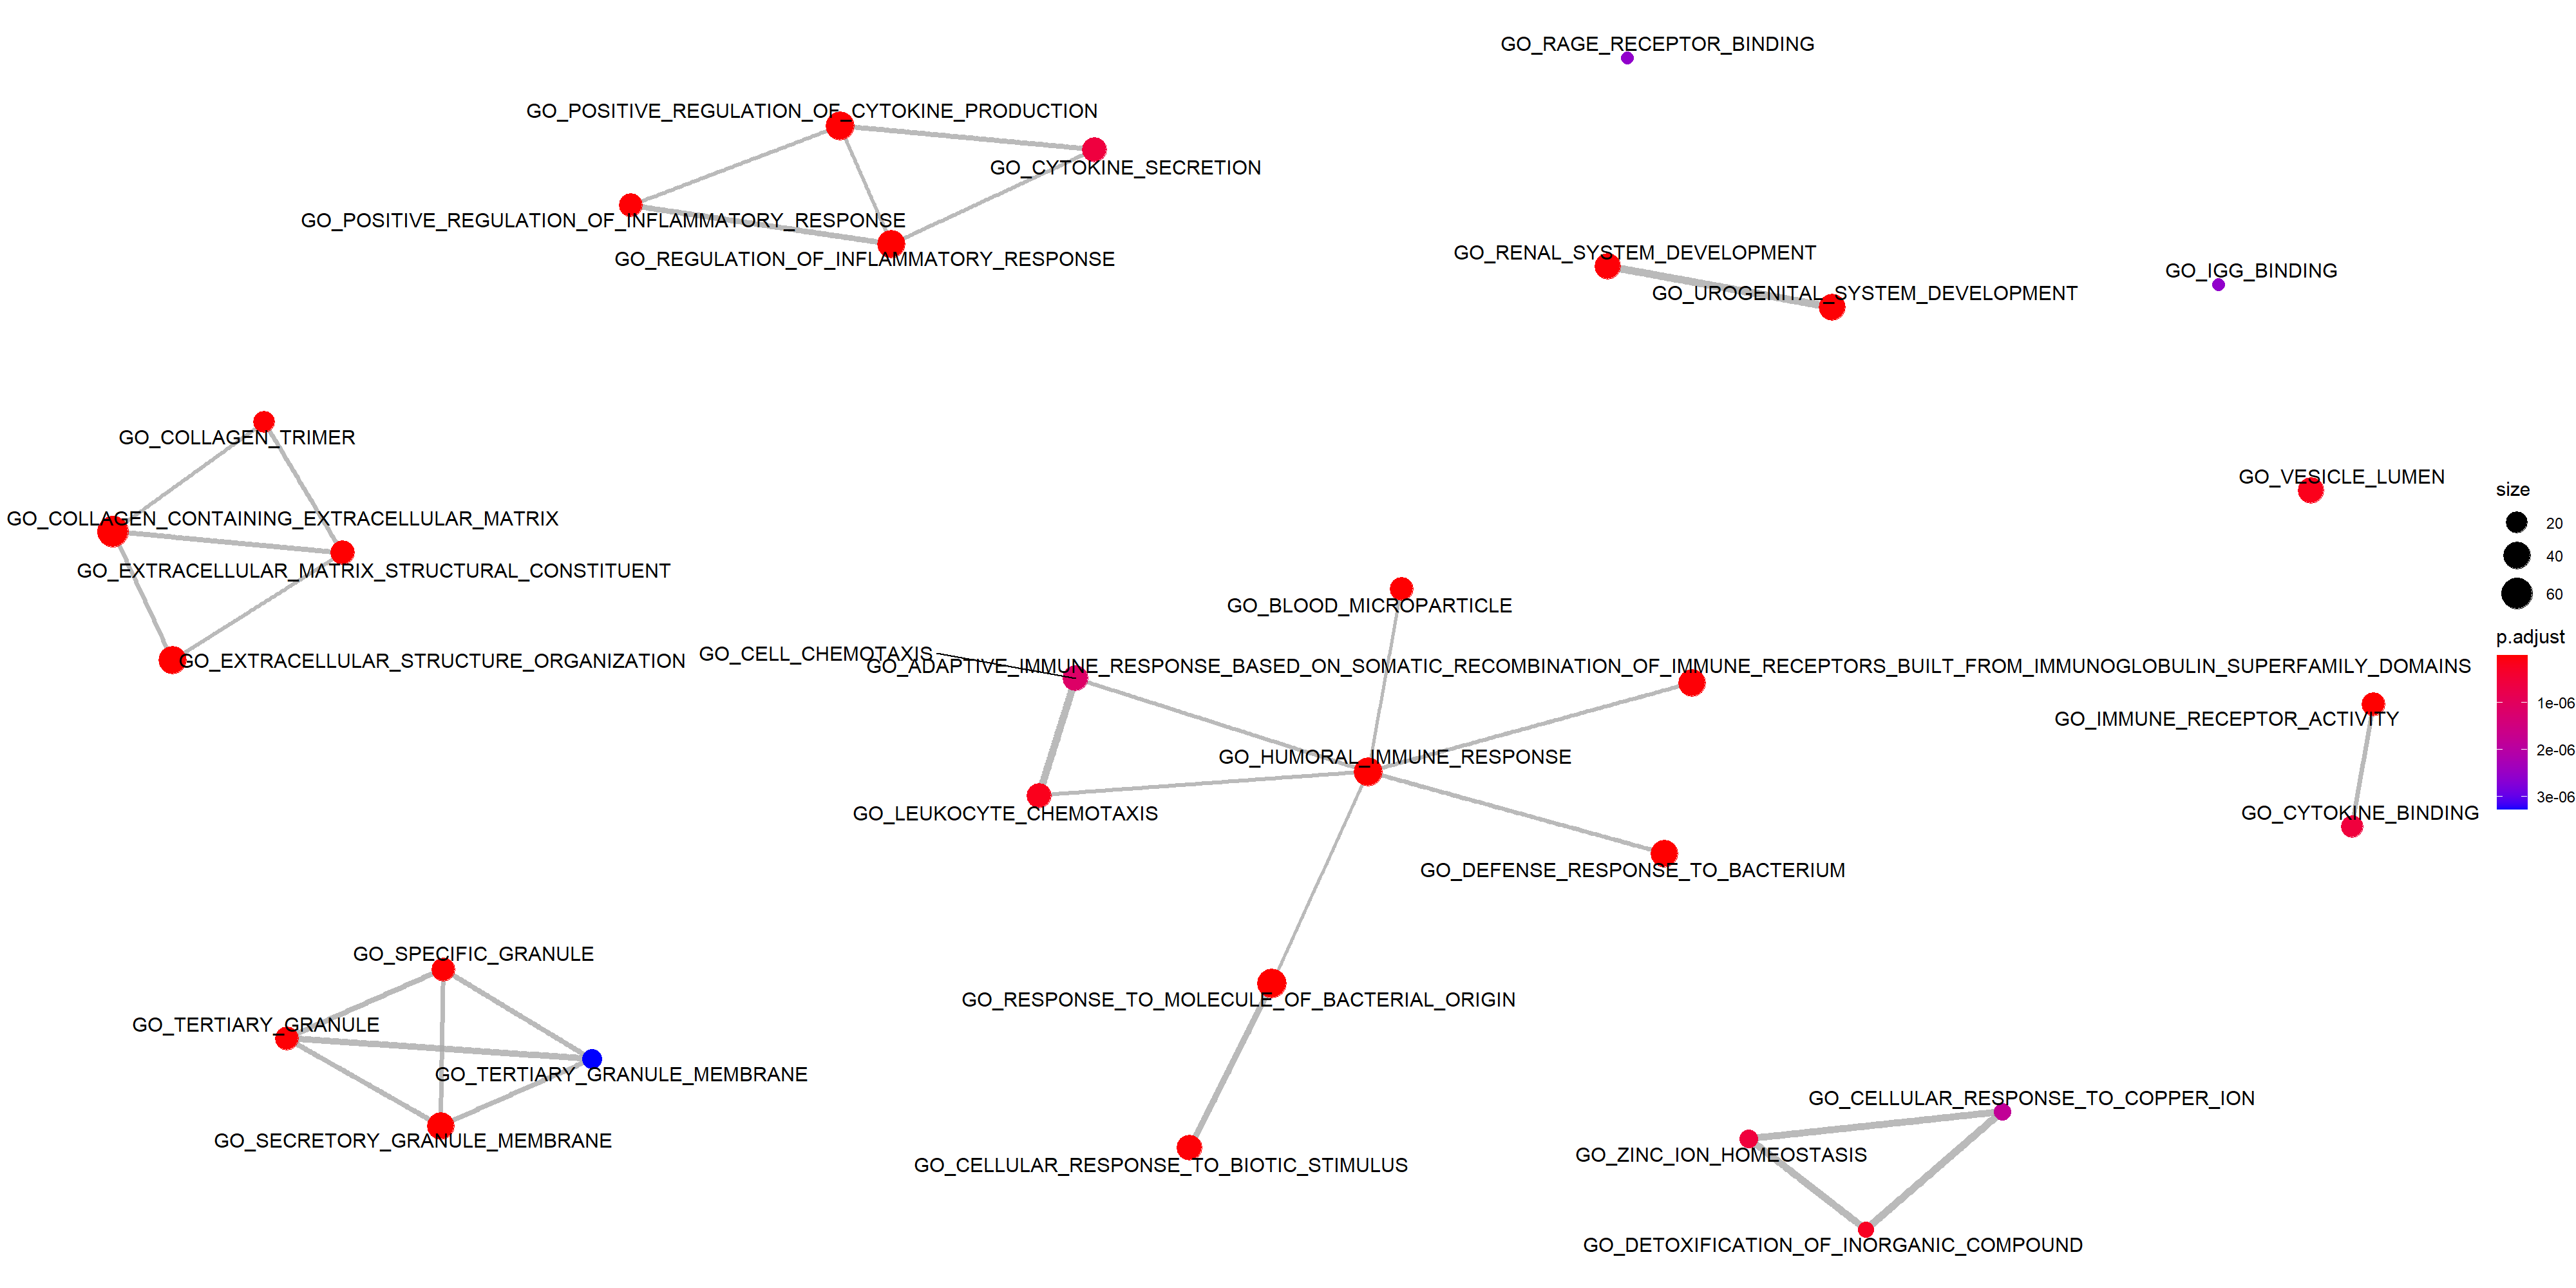
\includegraphics[width=10cm]{Figures/GSEA/CTLvsHD_emapplot.png} }}%
    \\
    \subfloat[\centering Gene-concept network for ORA. ]{{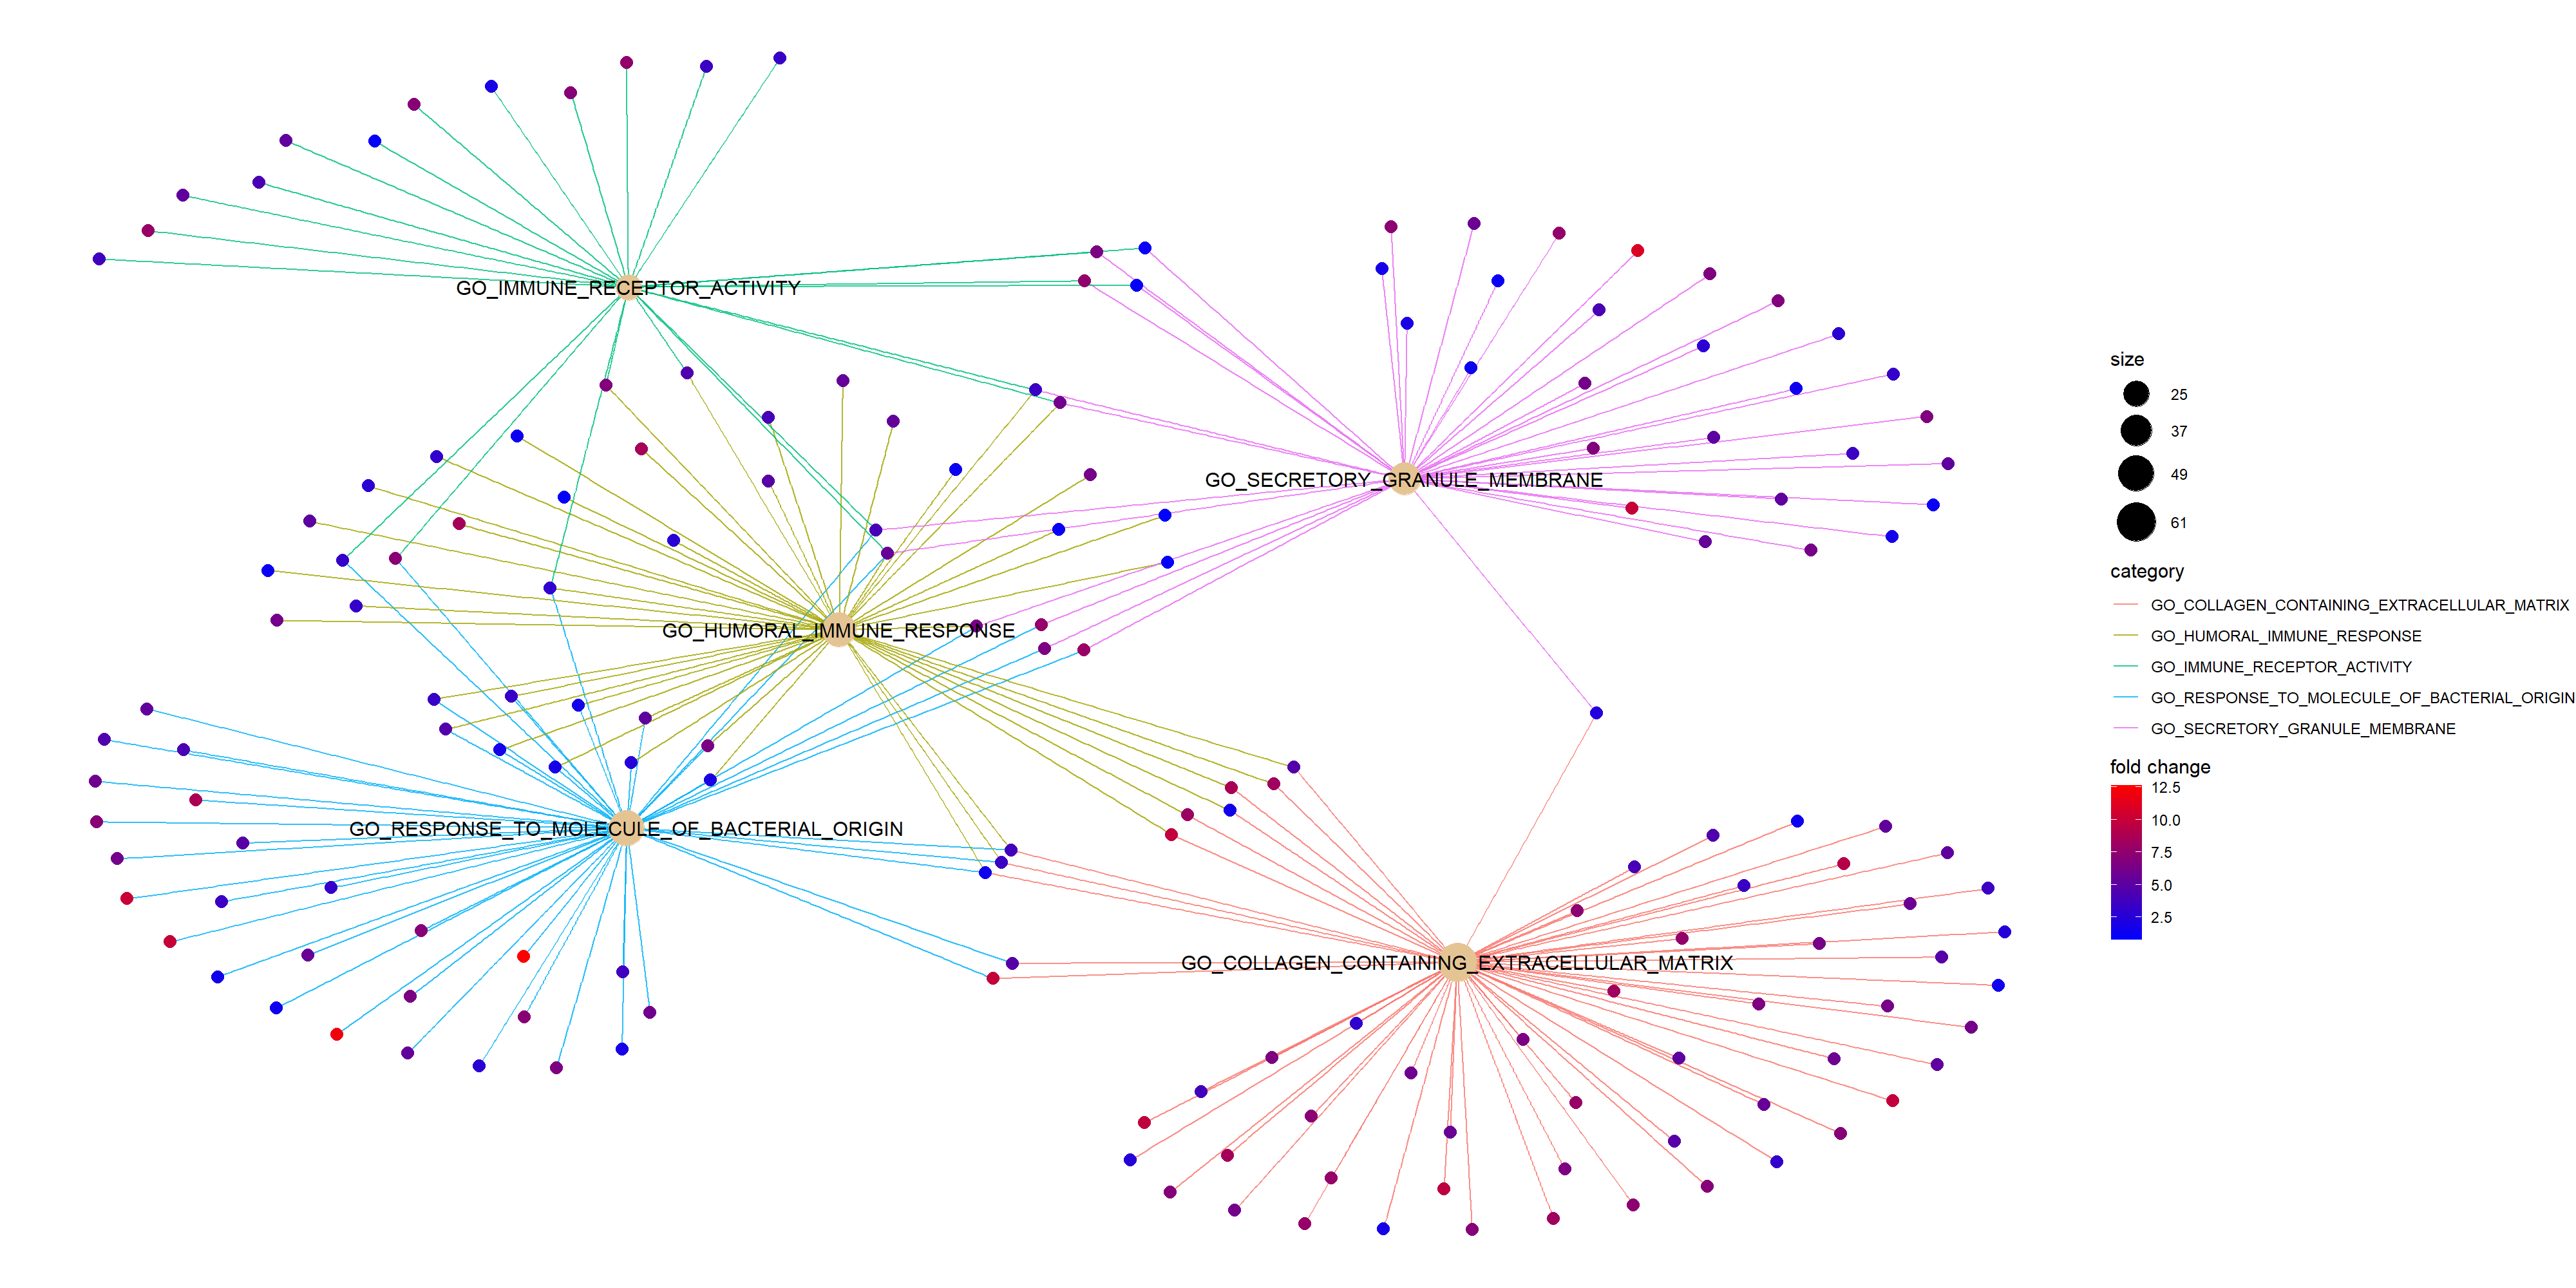
\includegraphics[width=10cm]{Figures/GSEA/CTLvsHD_cnetplot.png} }}%
    \\
    \subfloat[\centering Heatmap for ORA. ]{{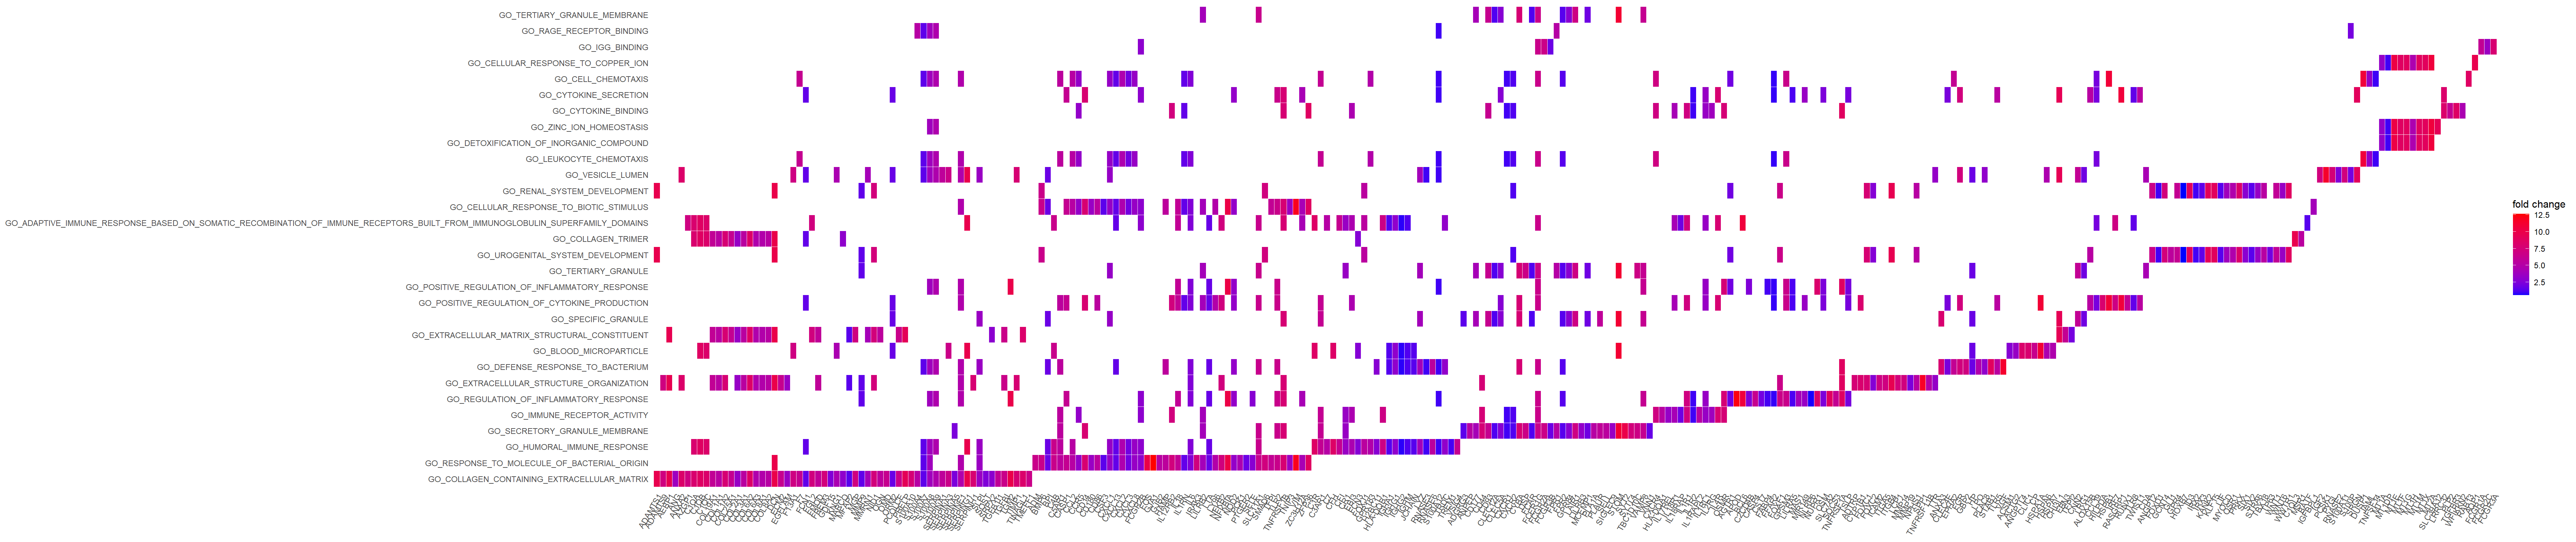
\includegraphics[width=10cm]{Figures/GSEA/CTLvsHD_heatmap.png} }}%
\caption{Functional analysis visualizations of PCx-HD.}
\end{figure}

% HD-Blood-f
\begin{figure}[!ht]%
    \centering
    \subfloat[\centering Enrichment map for ORA. ]{{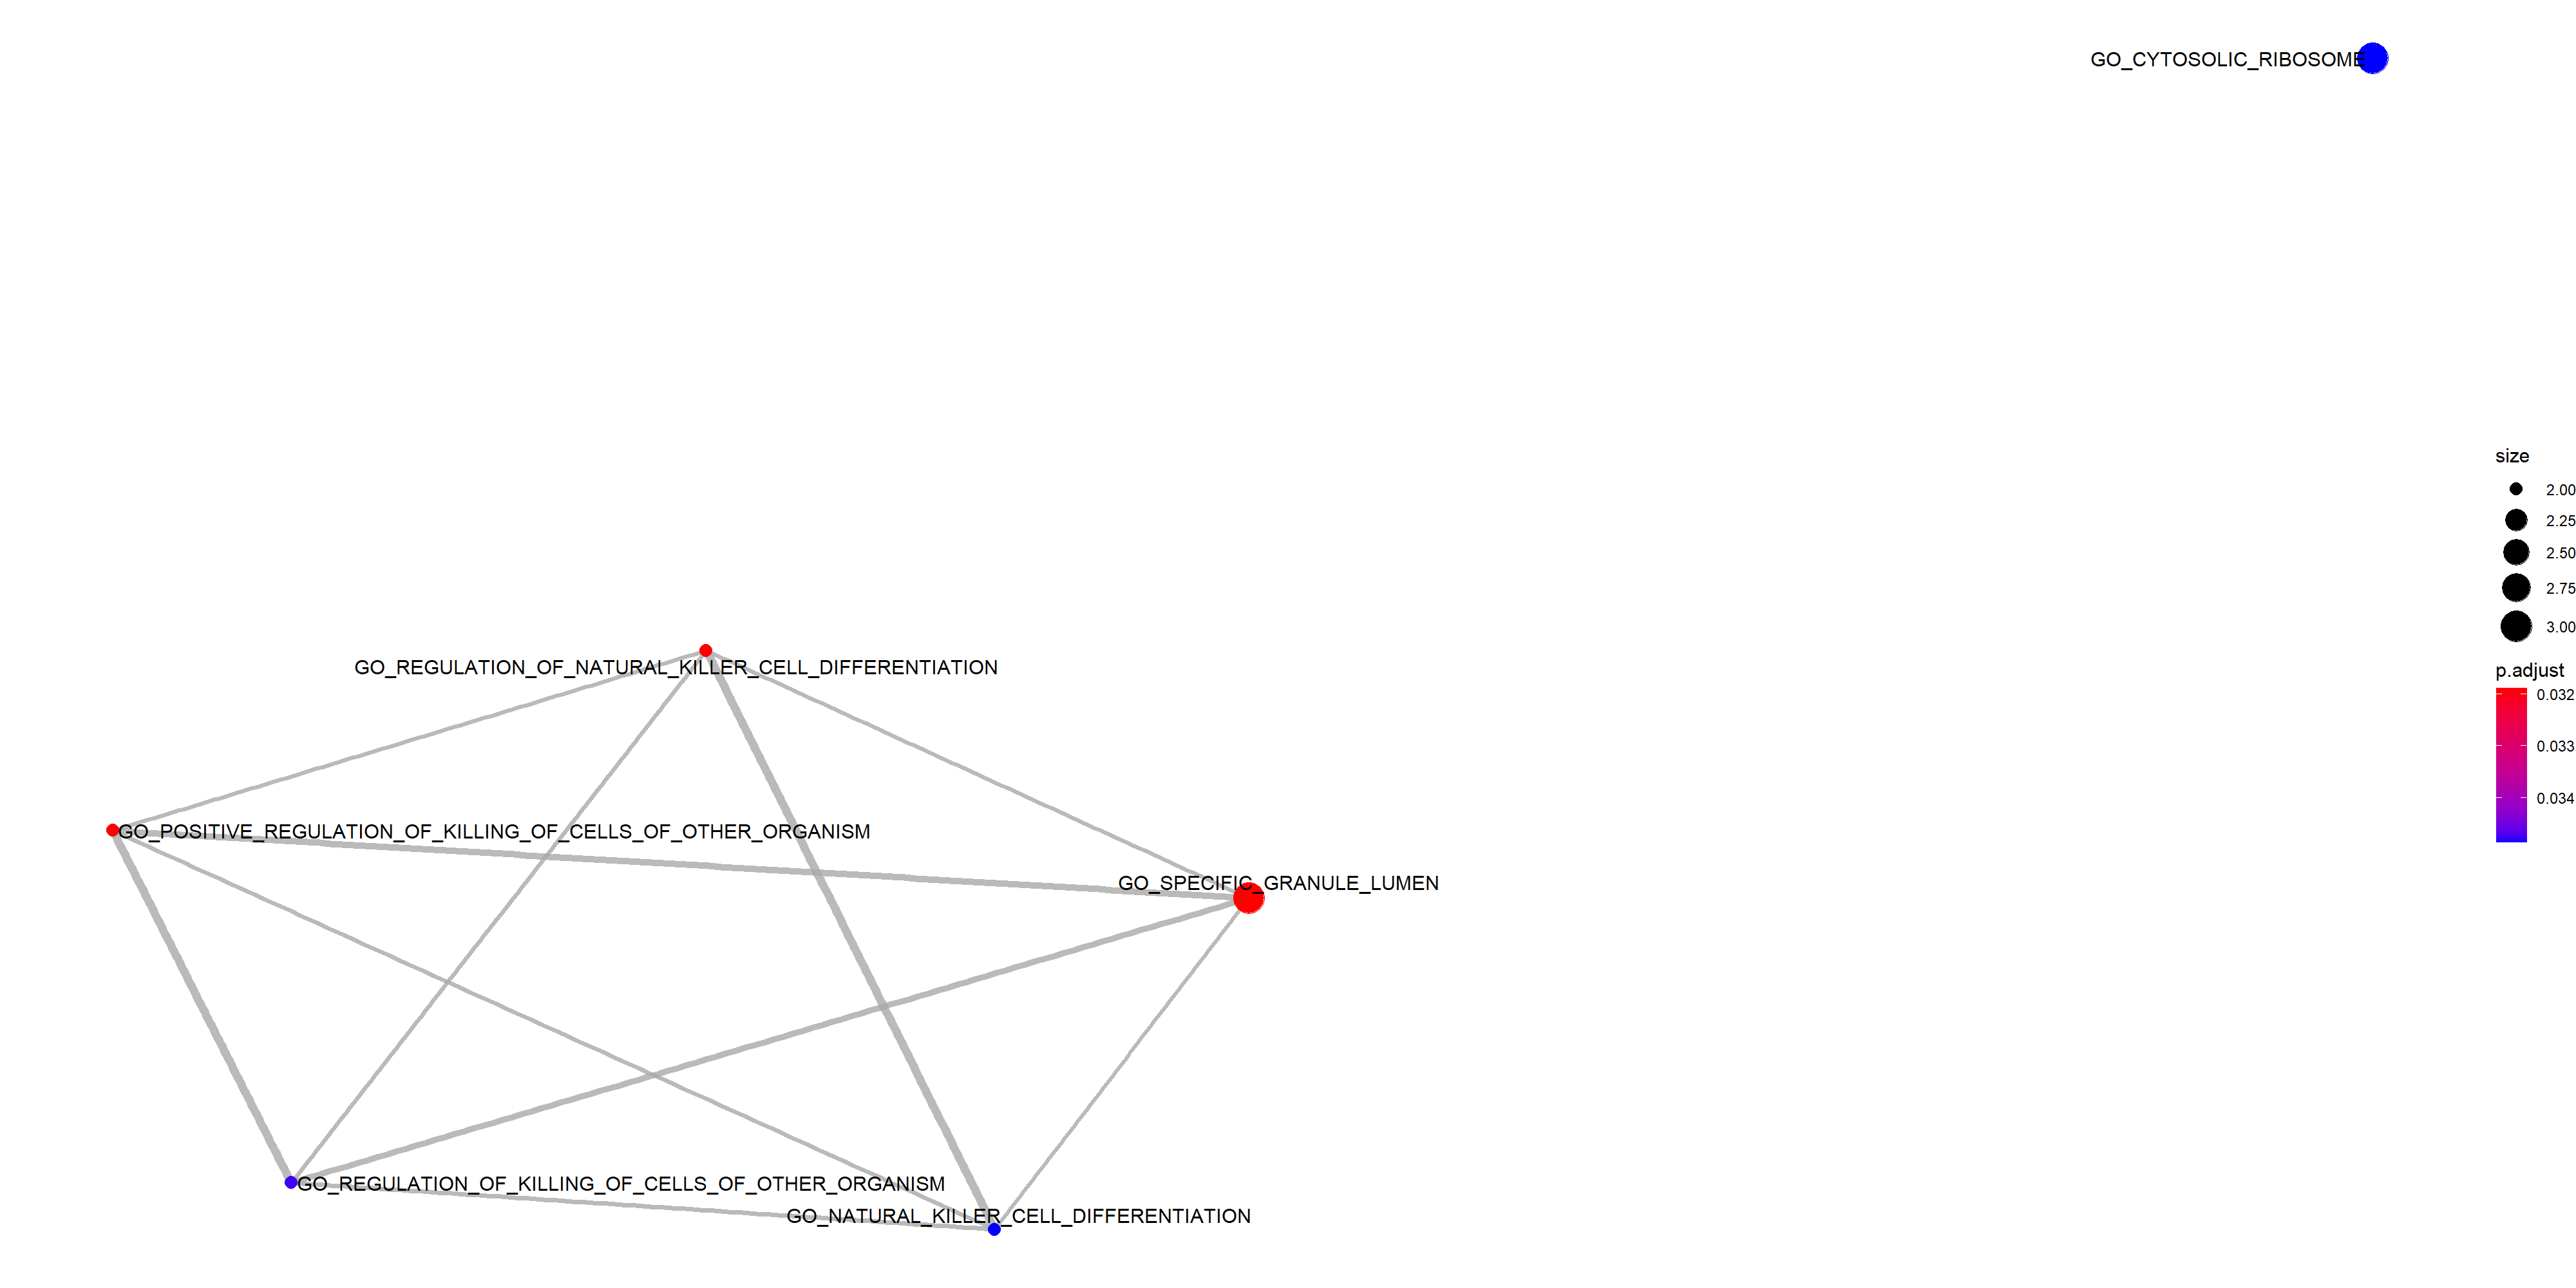
\includegraphics[width=10cm]{Figures/GSEA/CTLvsHD_ef_emapplot.png} }}%
    \\
    \subfloat[\centering Gene-concept network for ORA. ]{{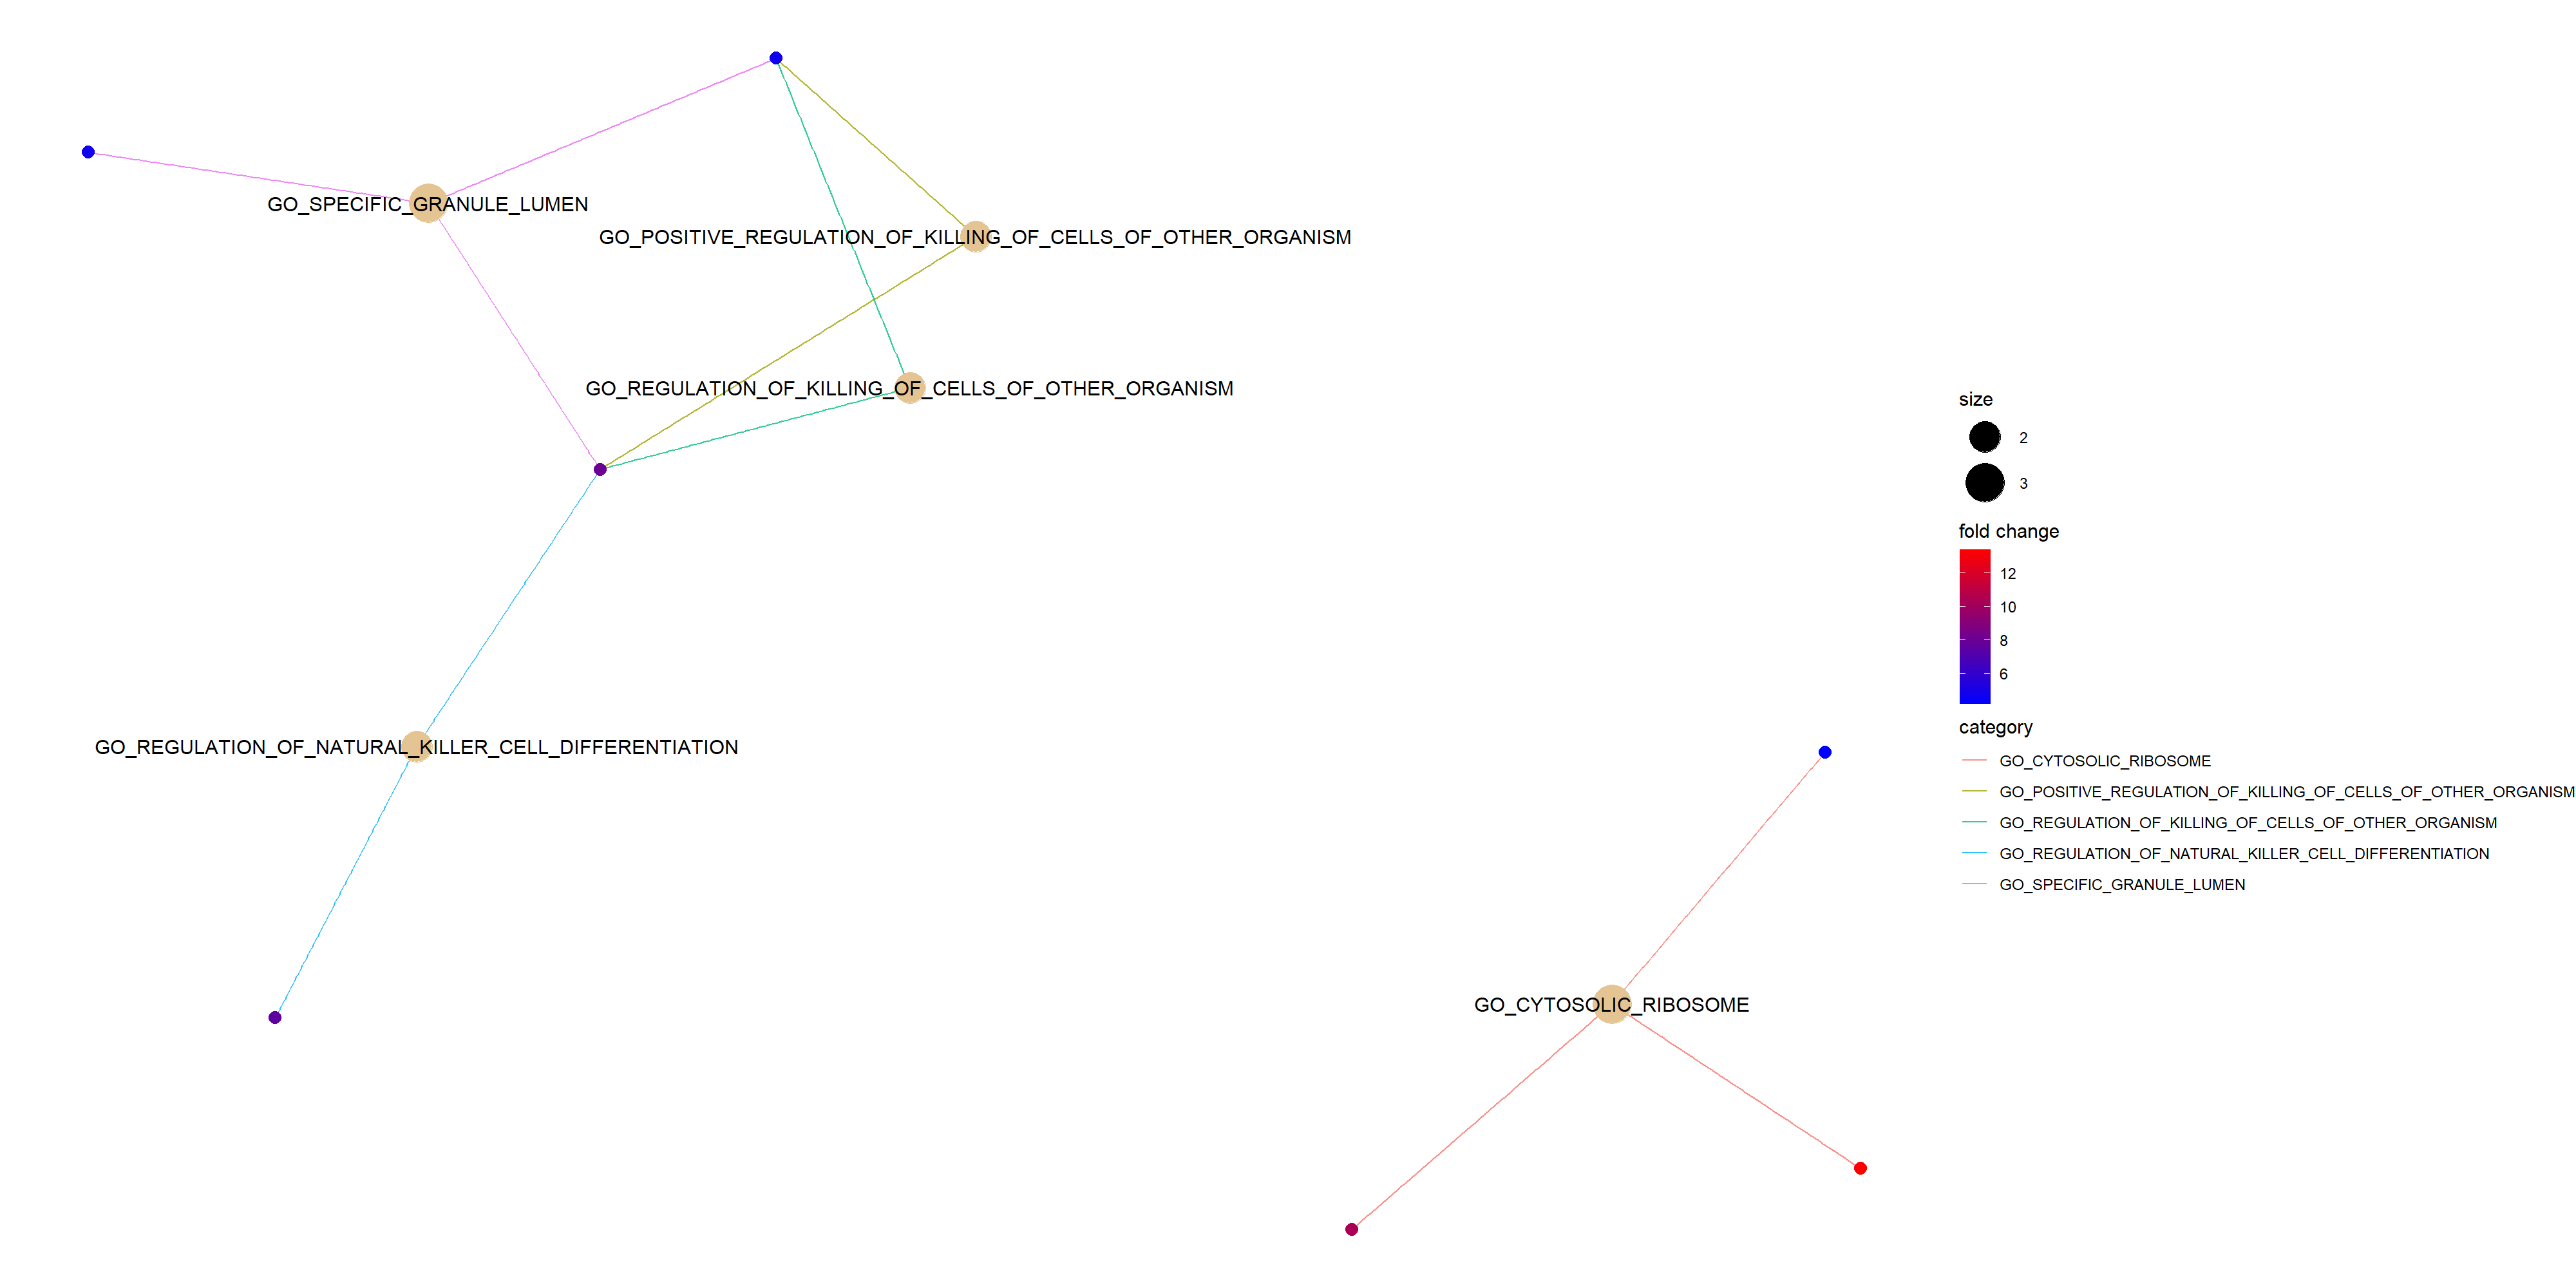
\includegraphics[width=10cm]{Figures/GSEA/CTLvsHD_ef_cnetplot.png} }}%
    \\
    \subfloat[\centering Heatmap for ORA. ]{{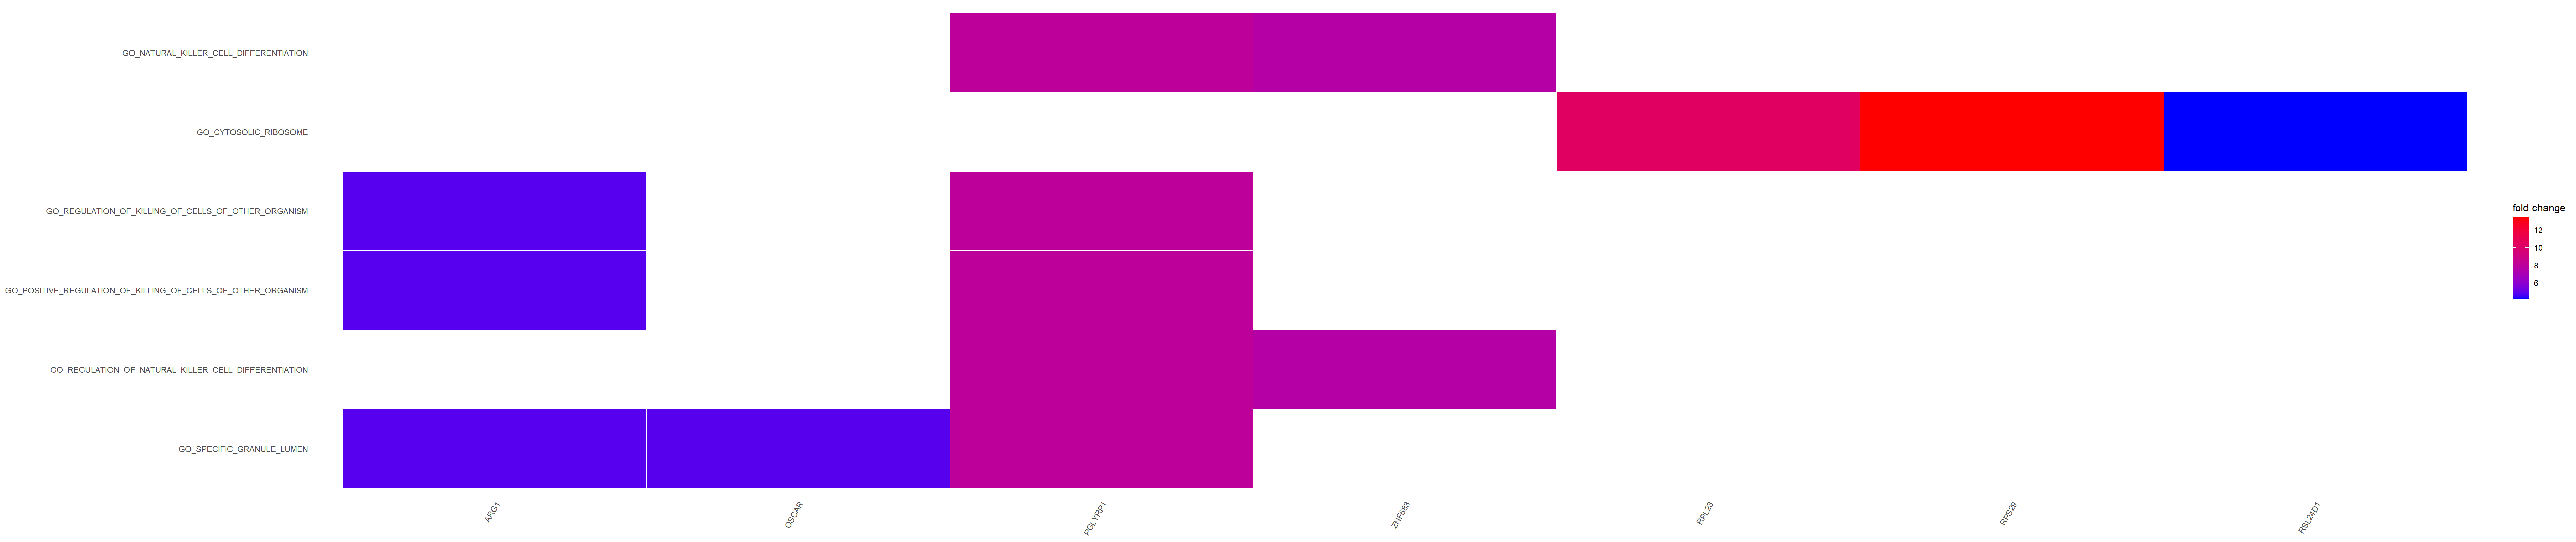
\includegraphics[width=10cm]{Figures/GSEA/CTLvsHD_ef_heatmap.png} }}%
\caption{Functional analysis visualizations of Blood-HD-f.}
\end{figure}

% HD-Blood-f-S1
\begin{figure}[!ht]%
    \centering
    \subfloat[\centering Enrichment map for ORA. ]{{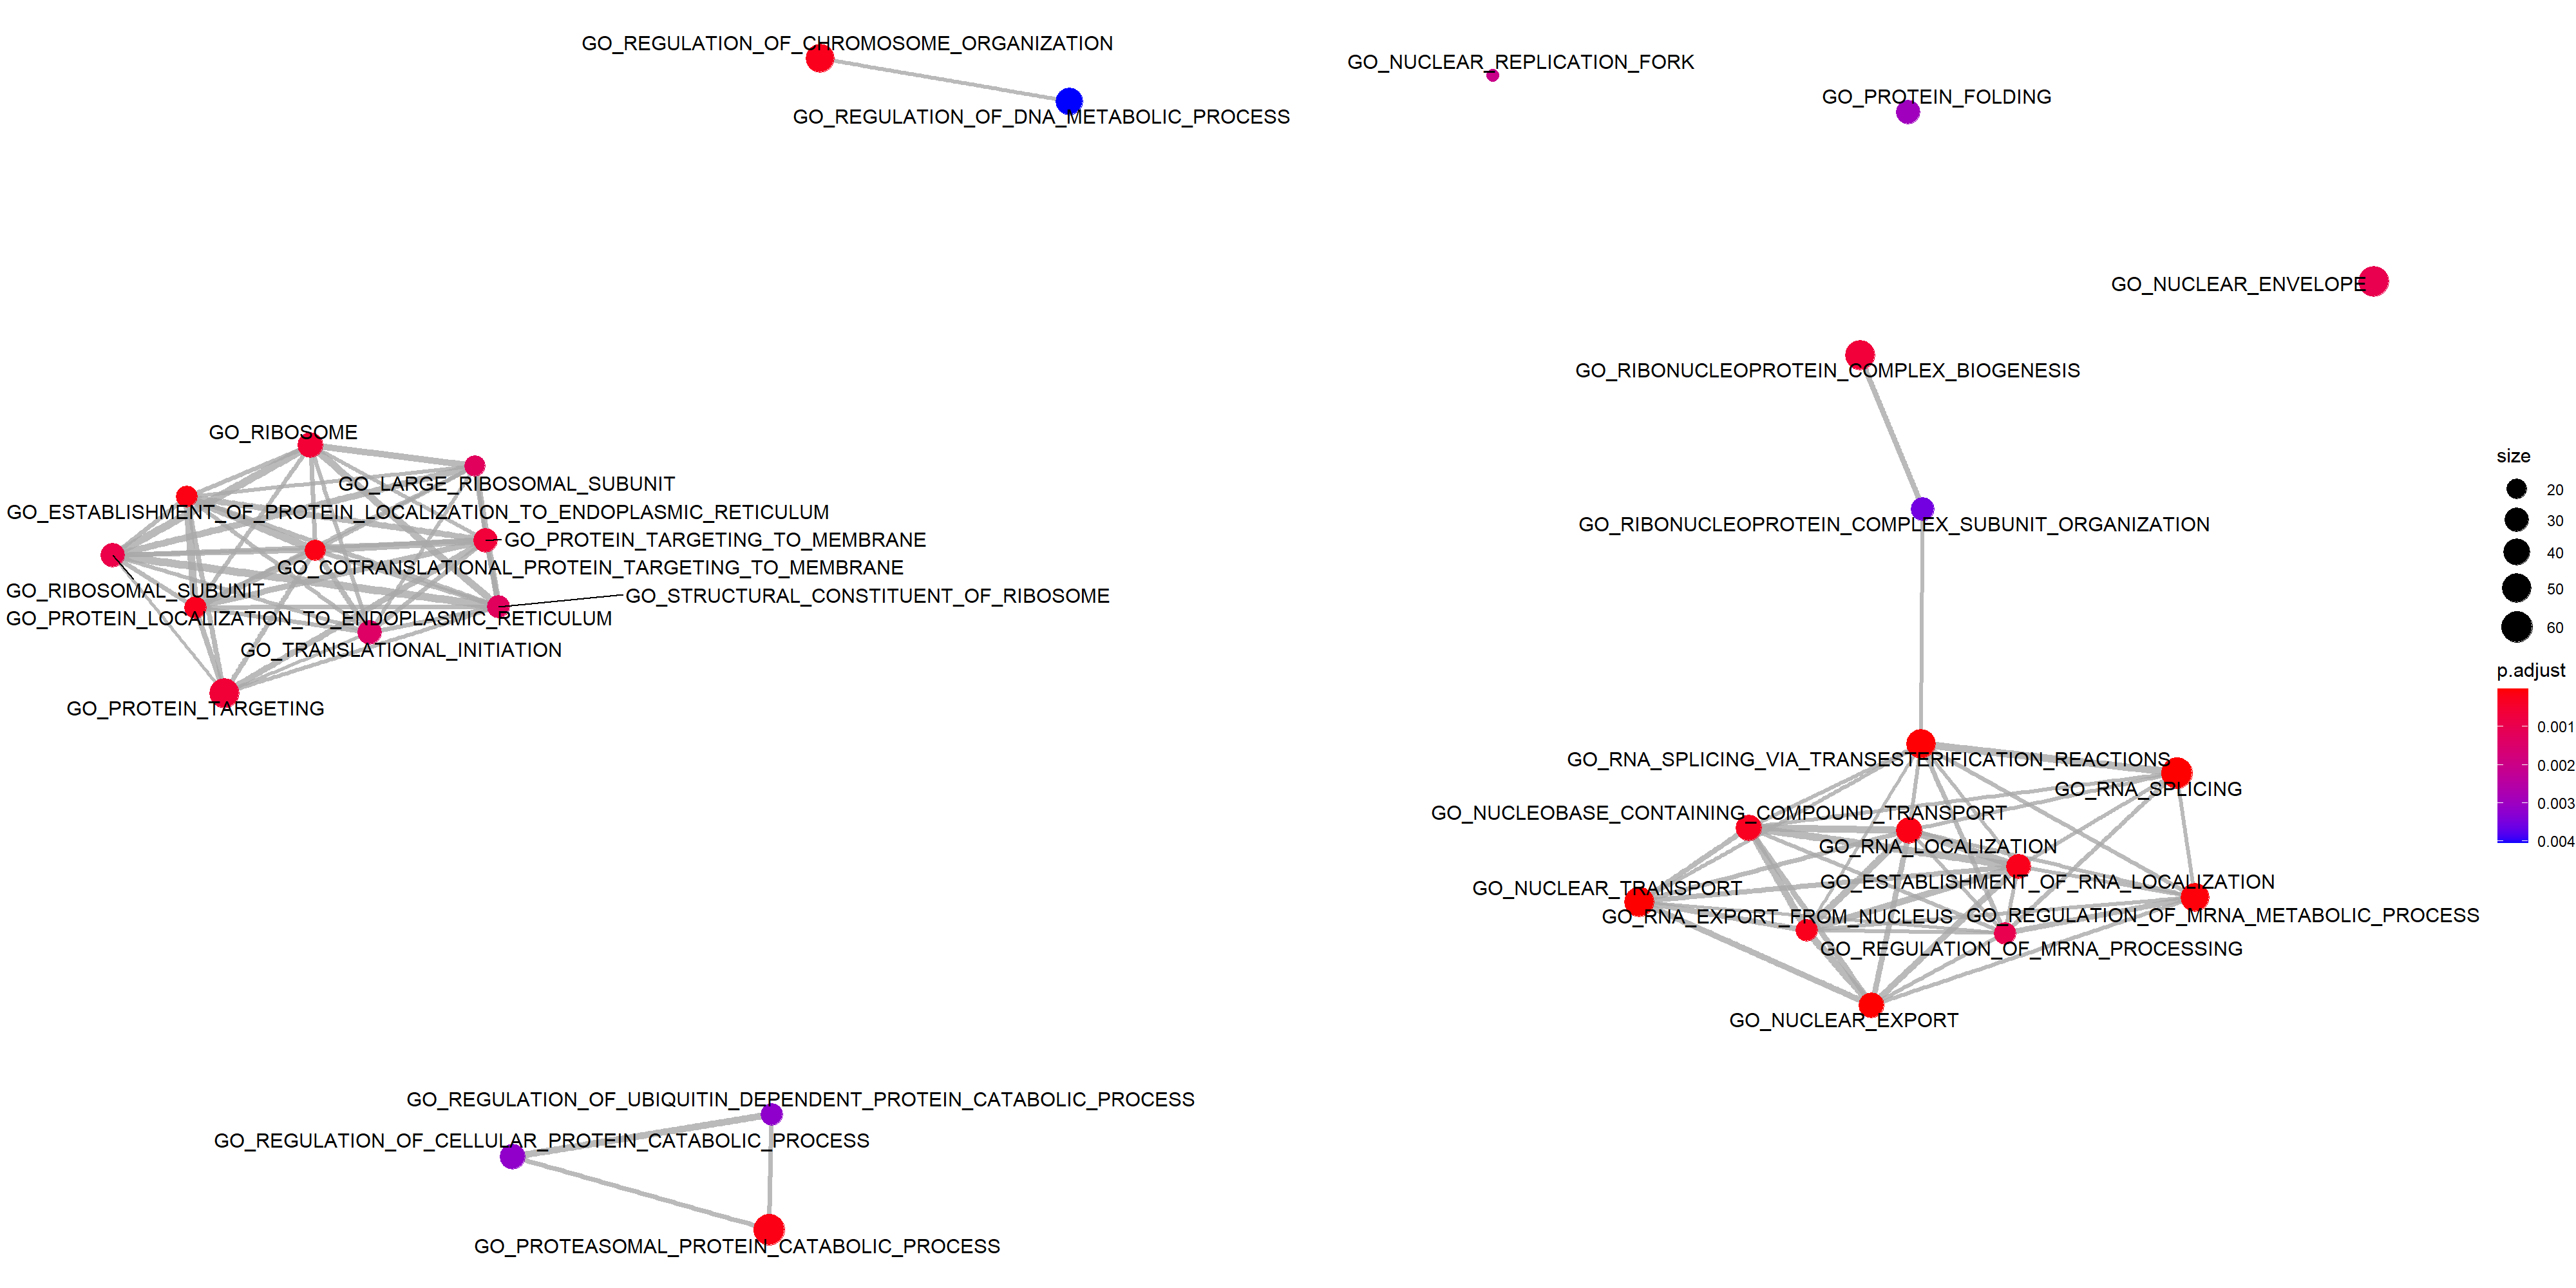
\includegraphics[width=10cm]{Figures/GSEA/CTLvs1bl_ef_emapplot.png} }}%
    \\
    \subfloat[\centering Gene-concept network for ORA. ]{{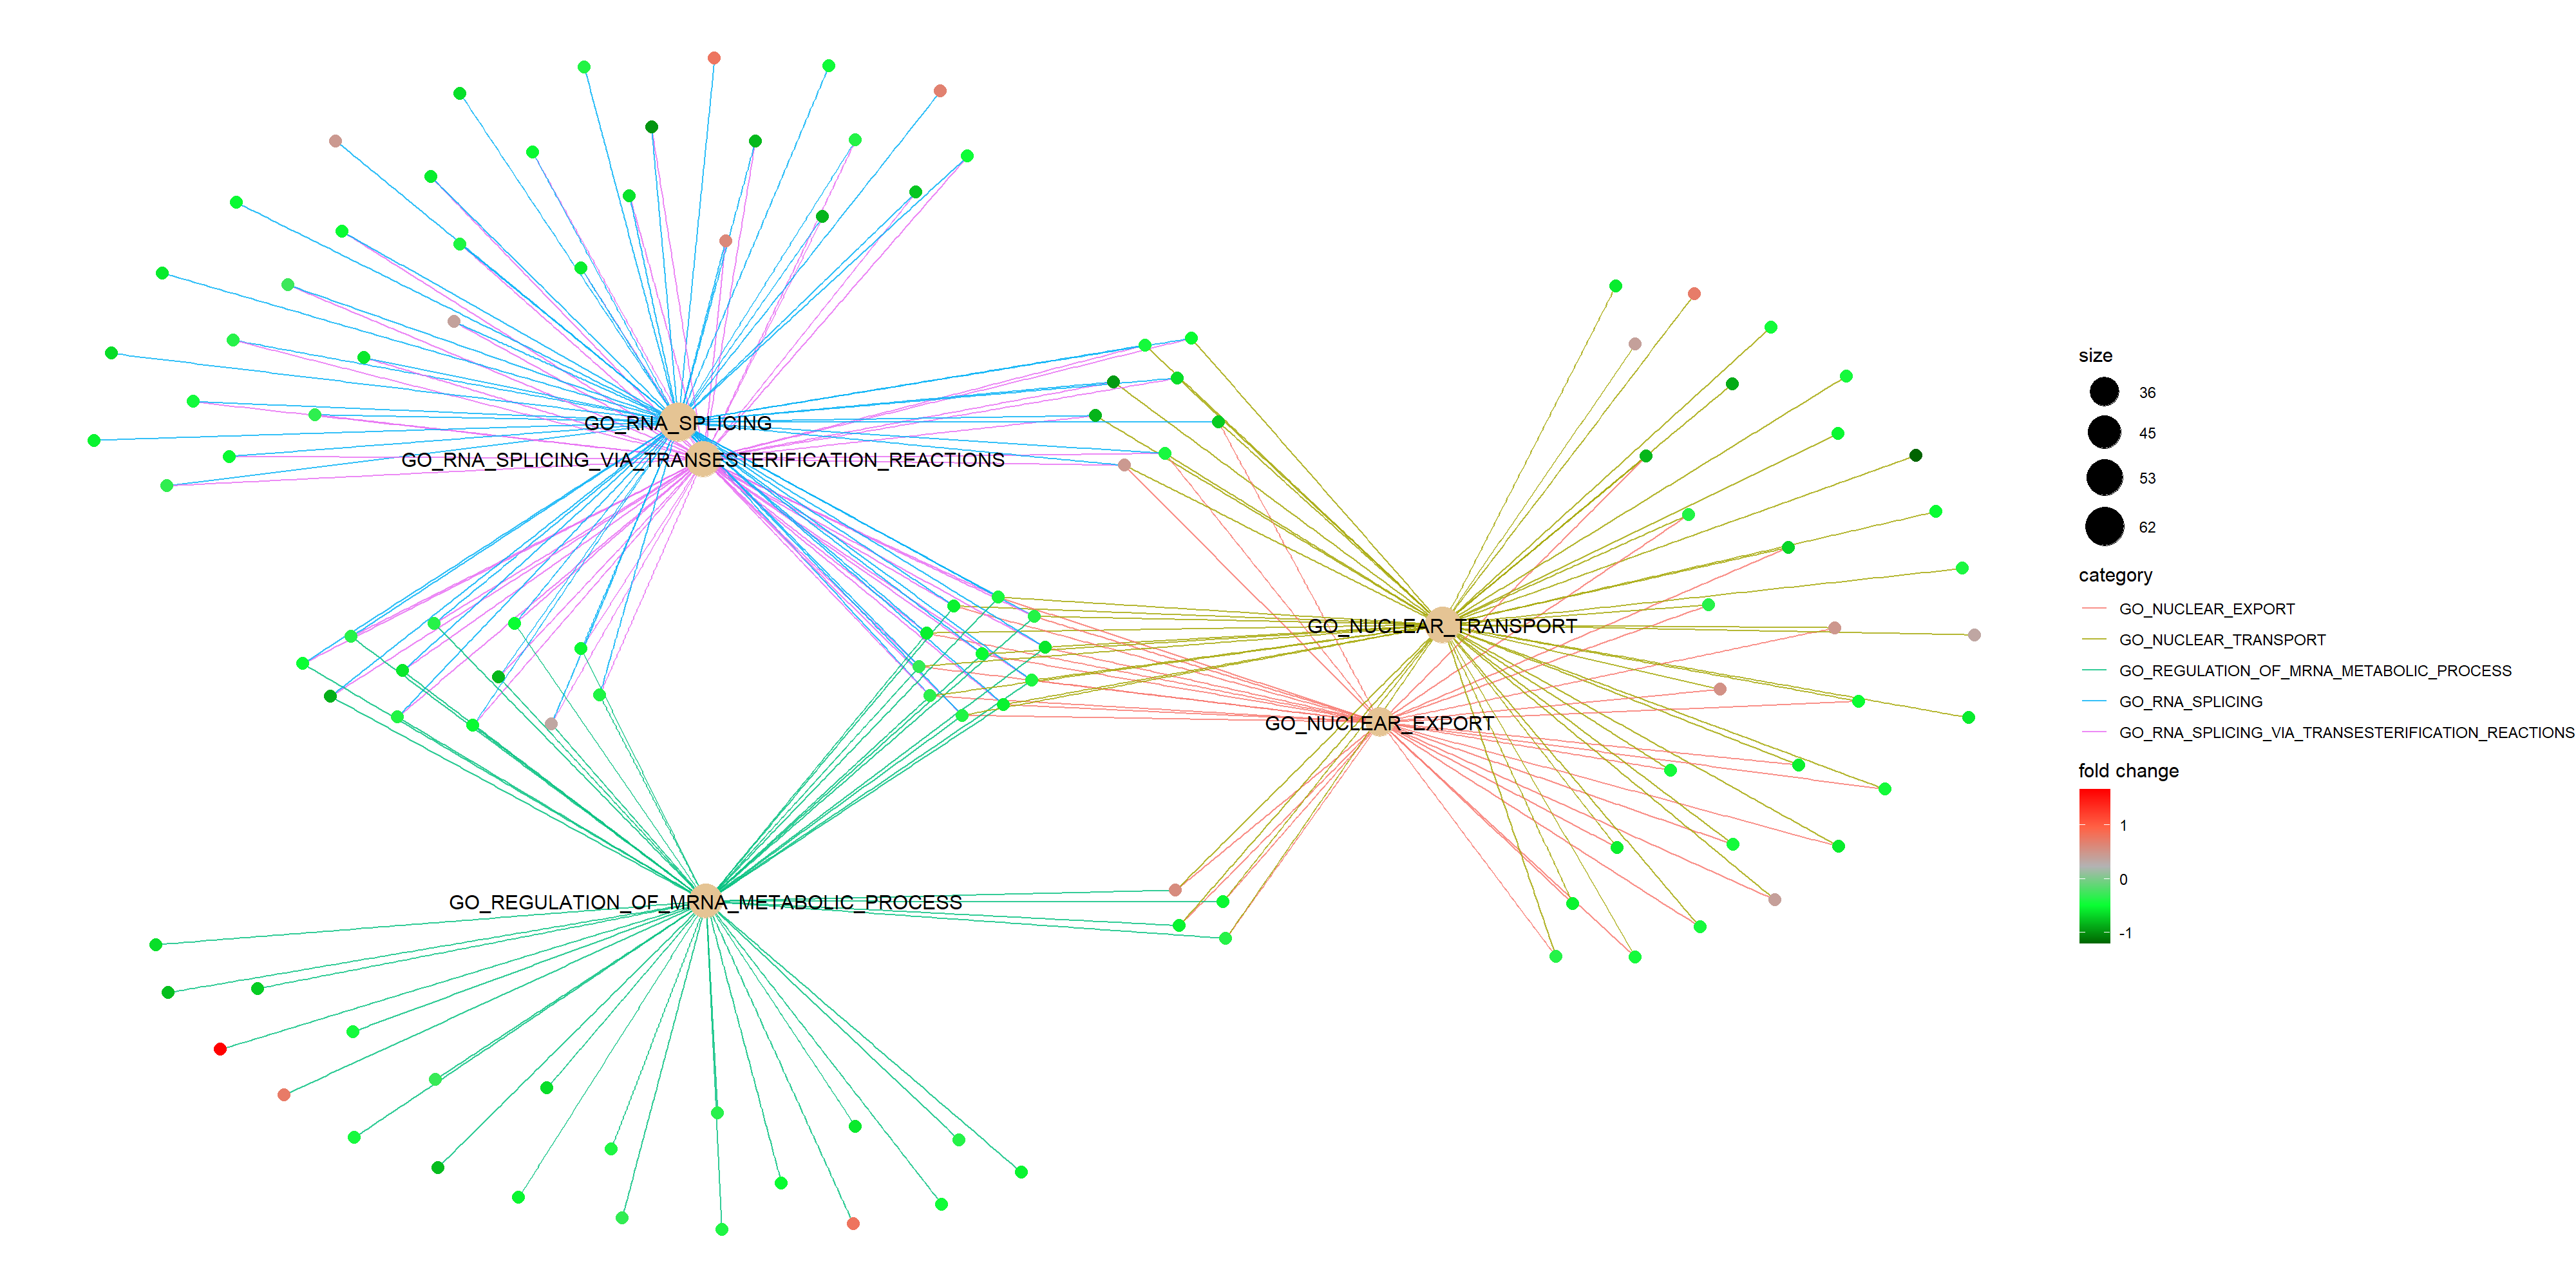
\includegraphics[width=10cm]{Figures/GSEA/CTLvs1bl_ef_cnetplot.png} }}%
    \\
    \subfloat[\centering Heatmap for ORA. ]{{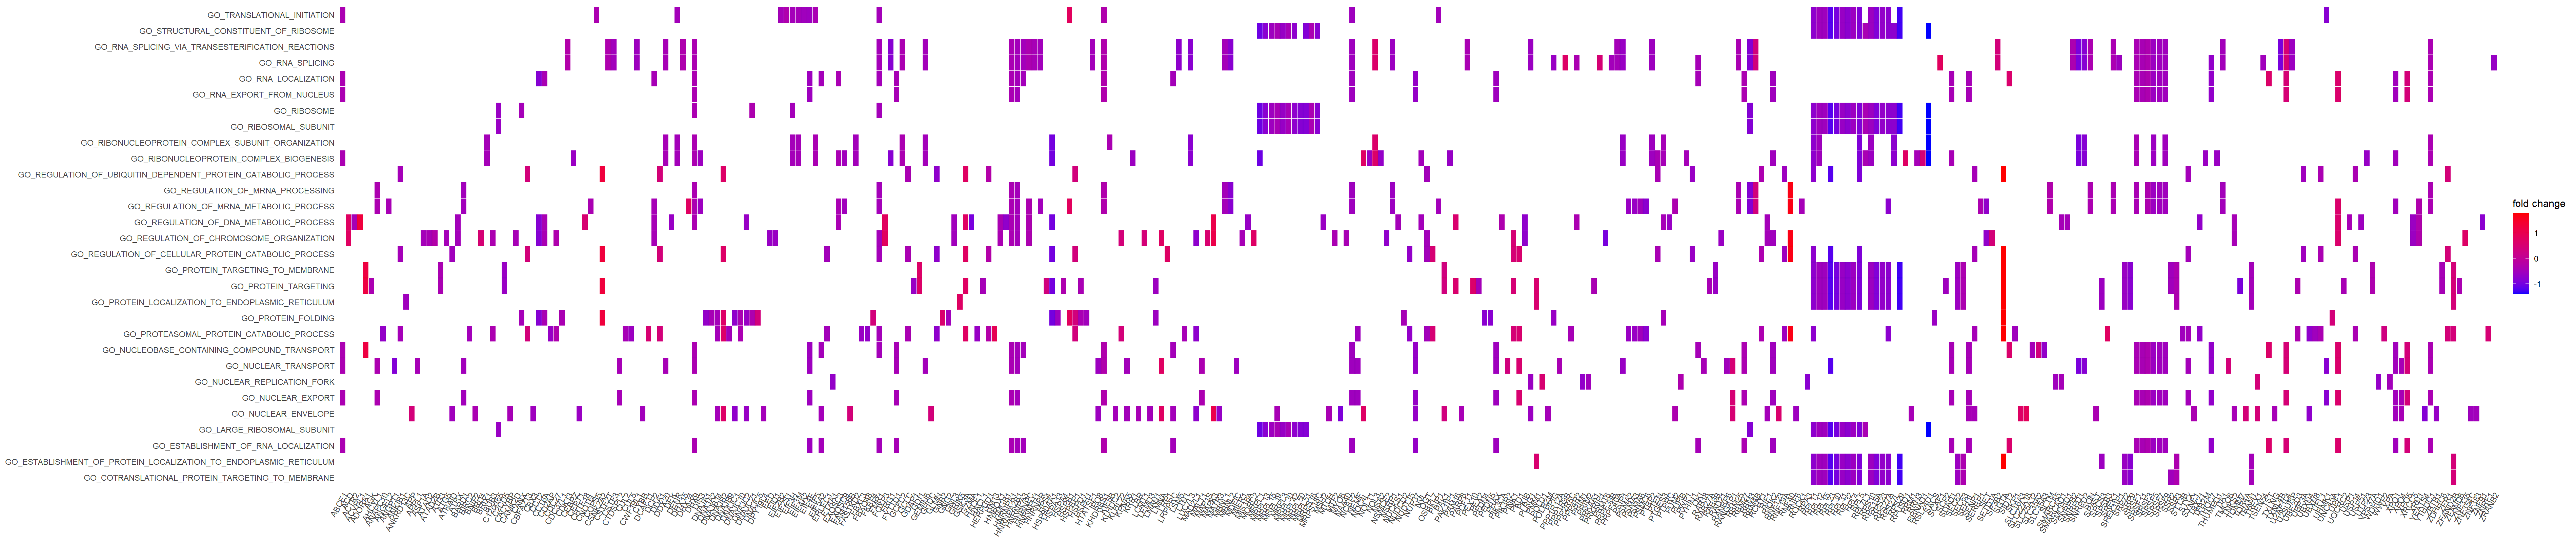
\includegraphics[width=10cm]{Figures/GSEA/CTLvs1bl_ef_heatmap.png} }}%
\caption{Functional analysis visualizations of Blood-HD-f-S1.}
\end{figure}

% HD-Blood-f-S2
\begin{figure}[!ht]%
    \centering
    \subfloat[\centering Enrichment map for ORA. ]{{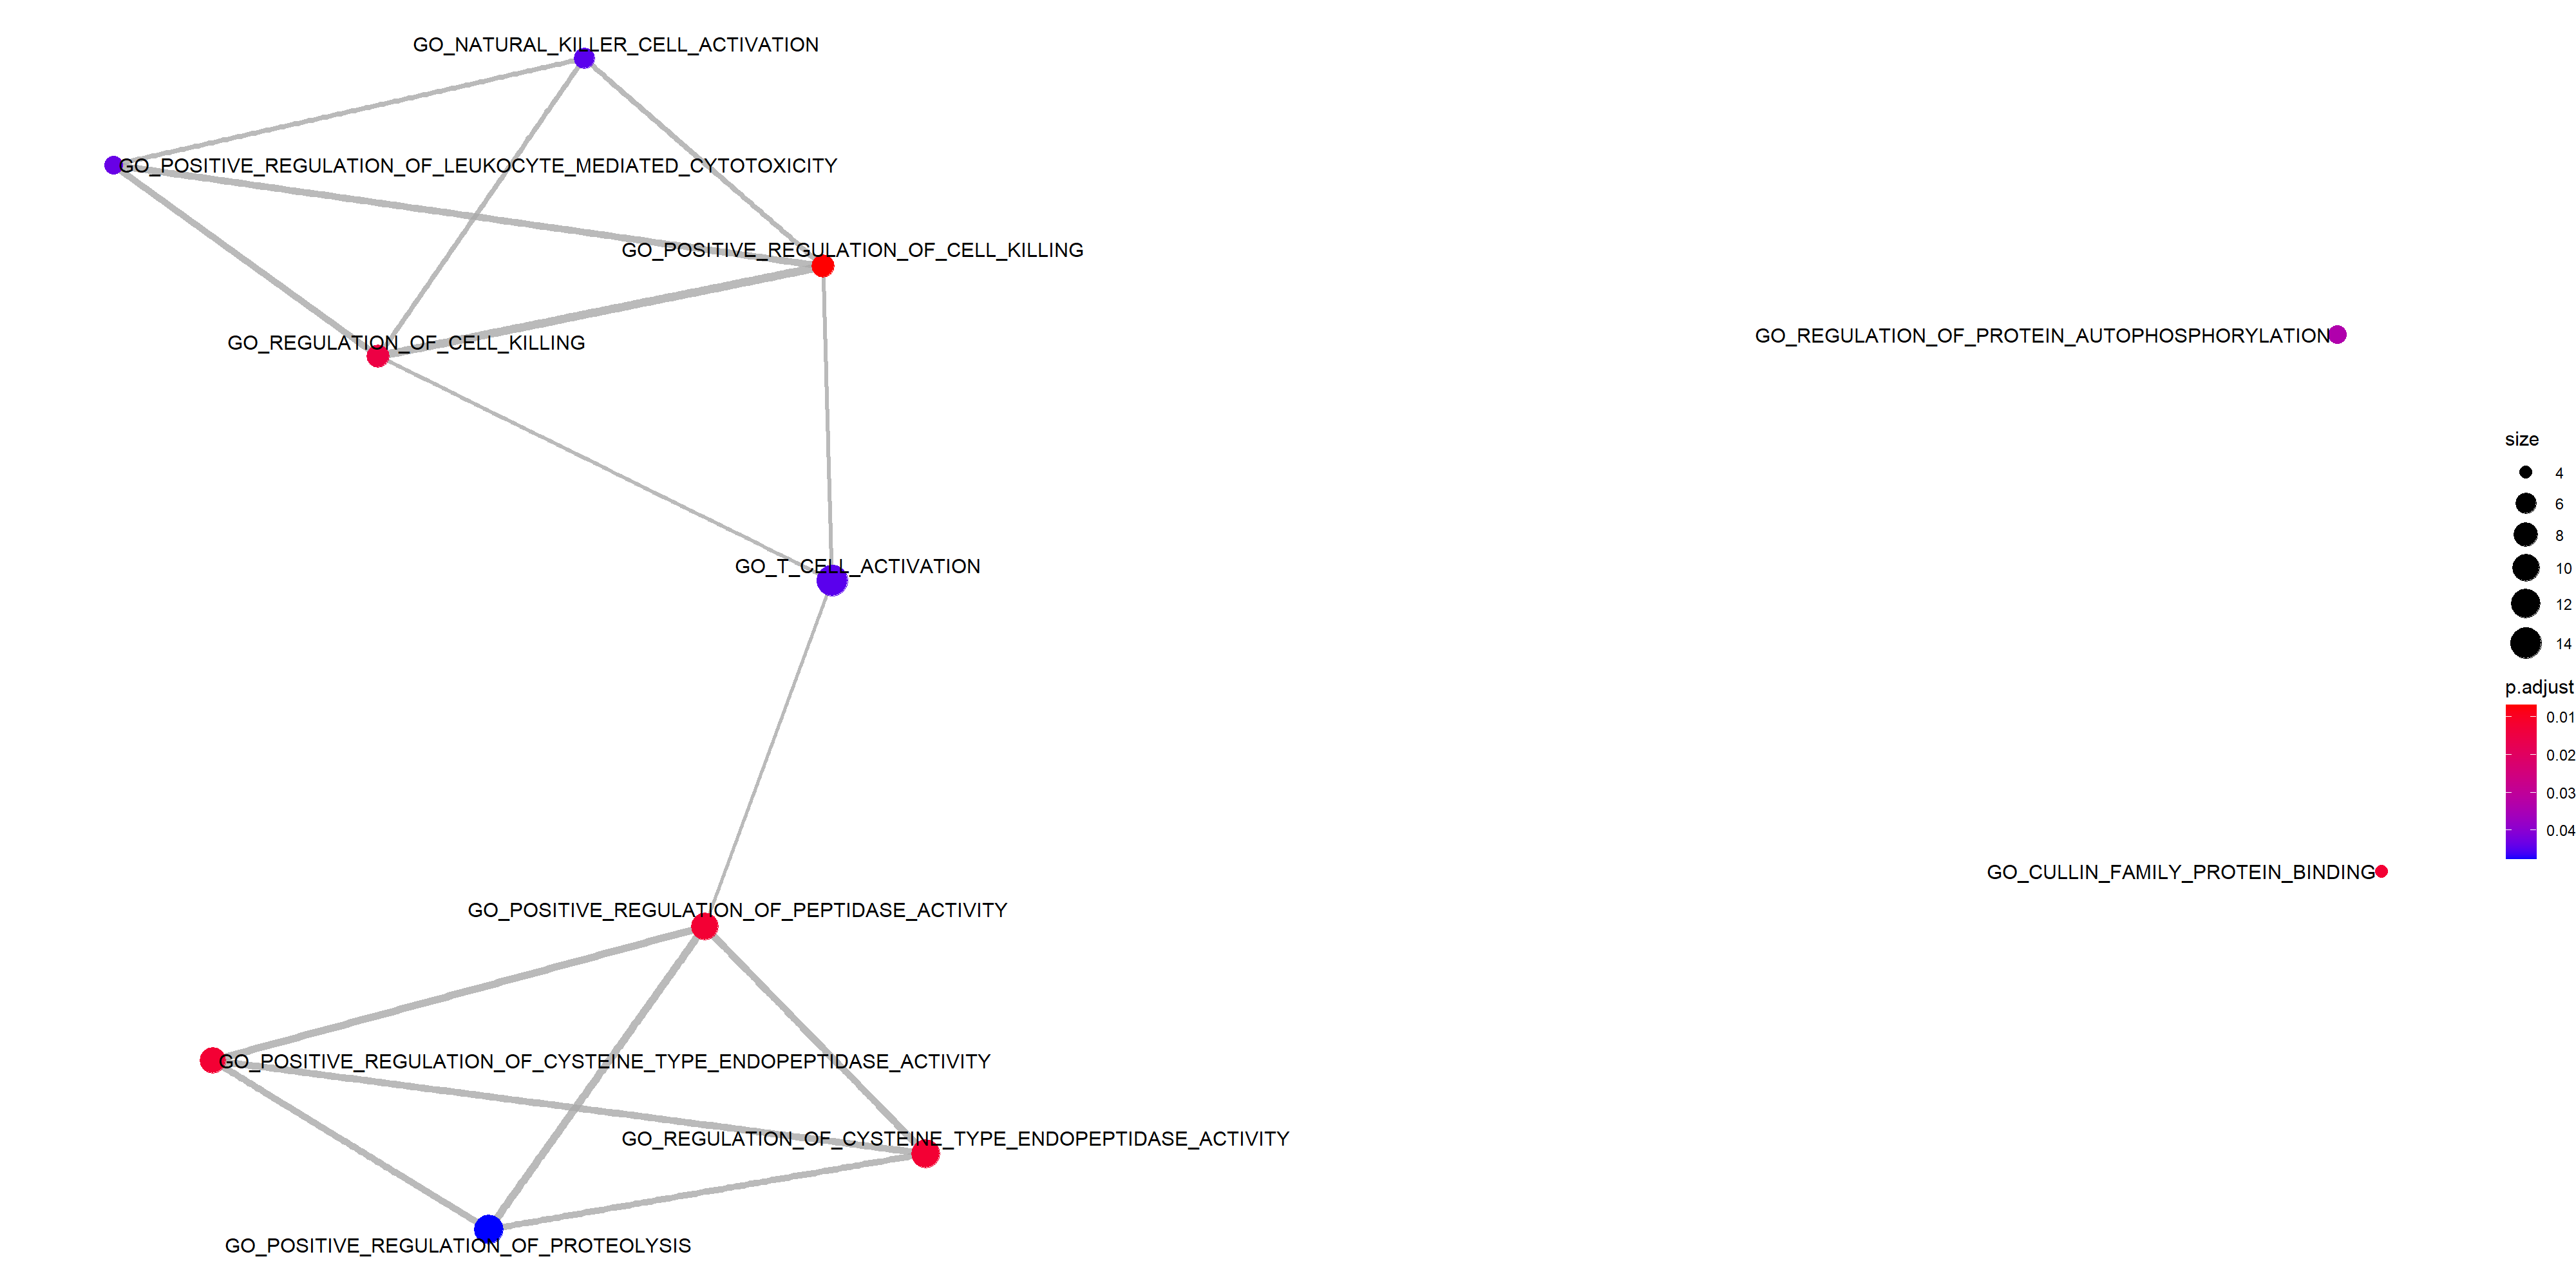
\includegraphics[width=10cm]{Figures/GSEA/CTLvs2bl_ef_emapplot.png} }}%
    \\
    \subfloat[\centering Gene-concept network for ORA. ]{{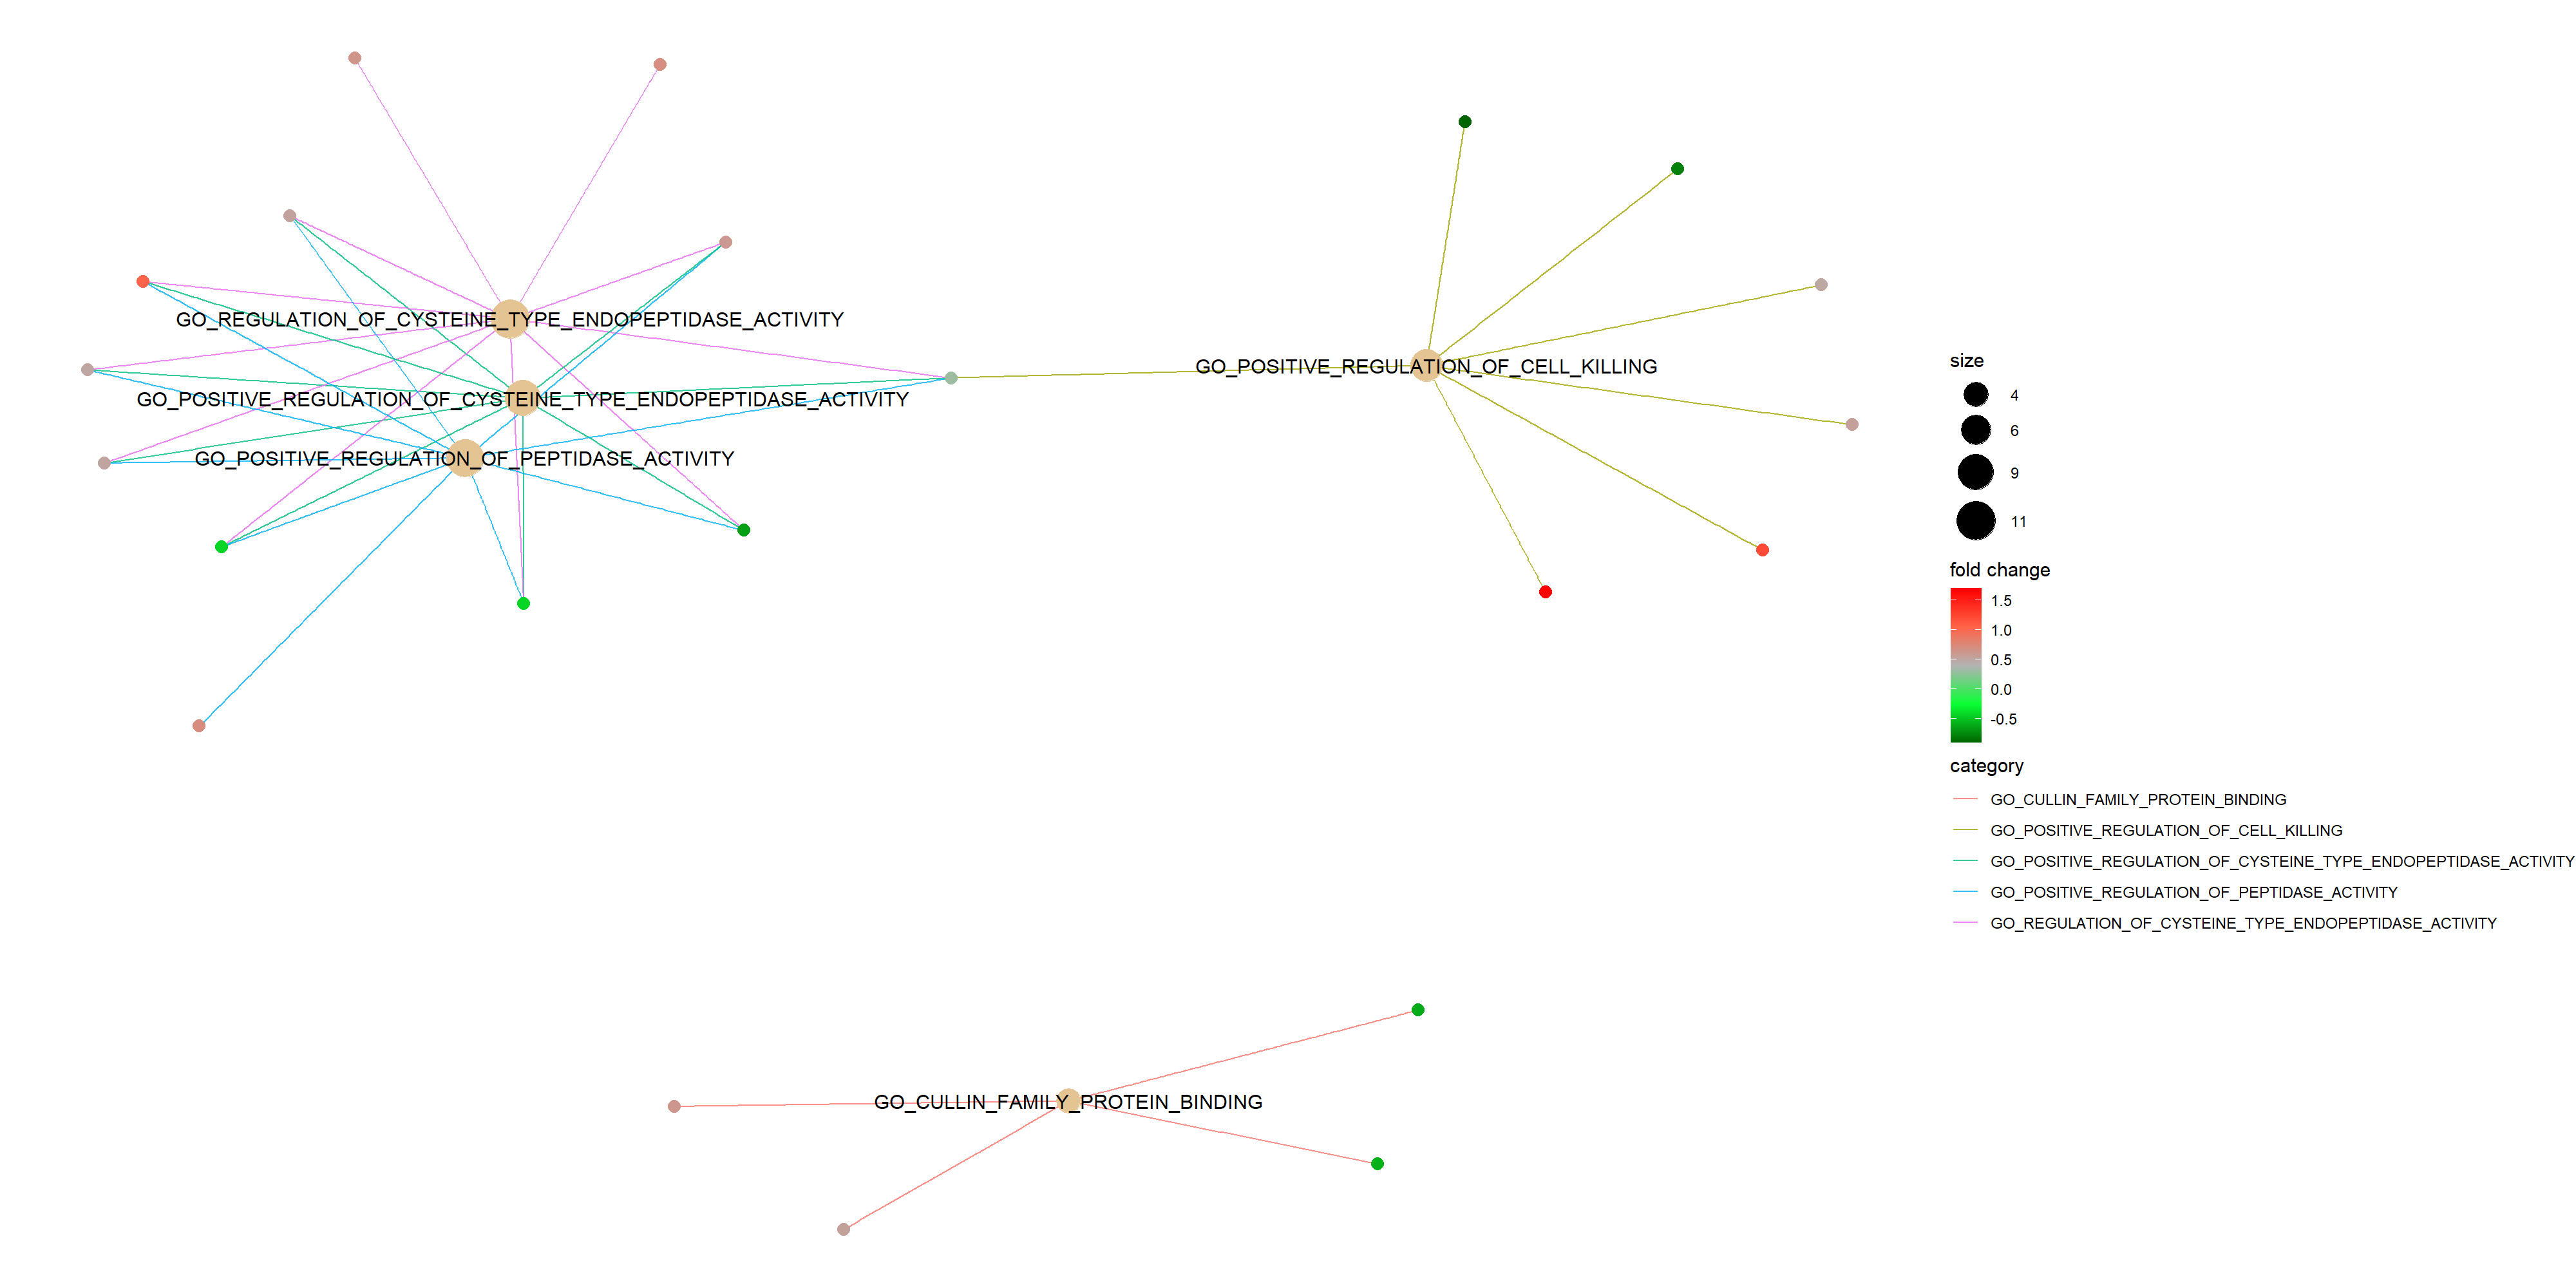
\includegraphics[width=10cm]{Figures/GSEA/CTLvs2bl_ef_cnetplot.png} }}%
    \\
    \subfloat[\centering Heatmap for ORA. ]{{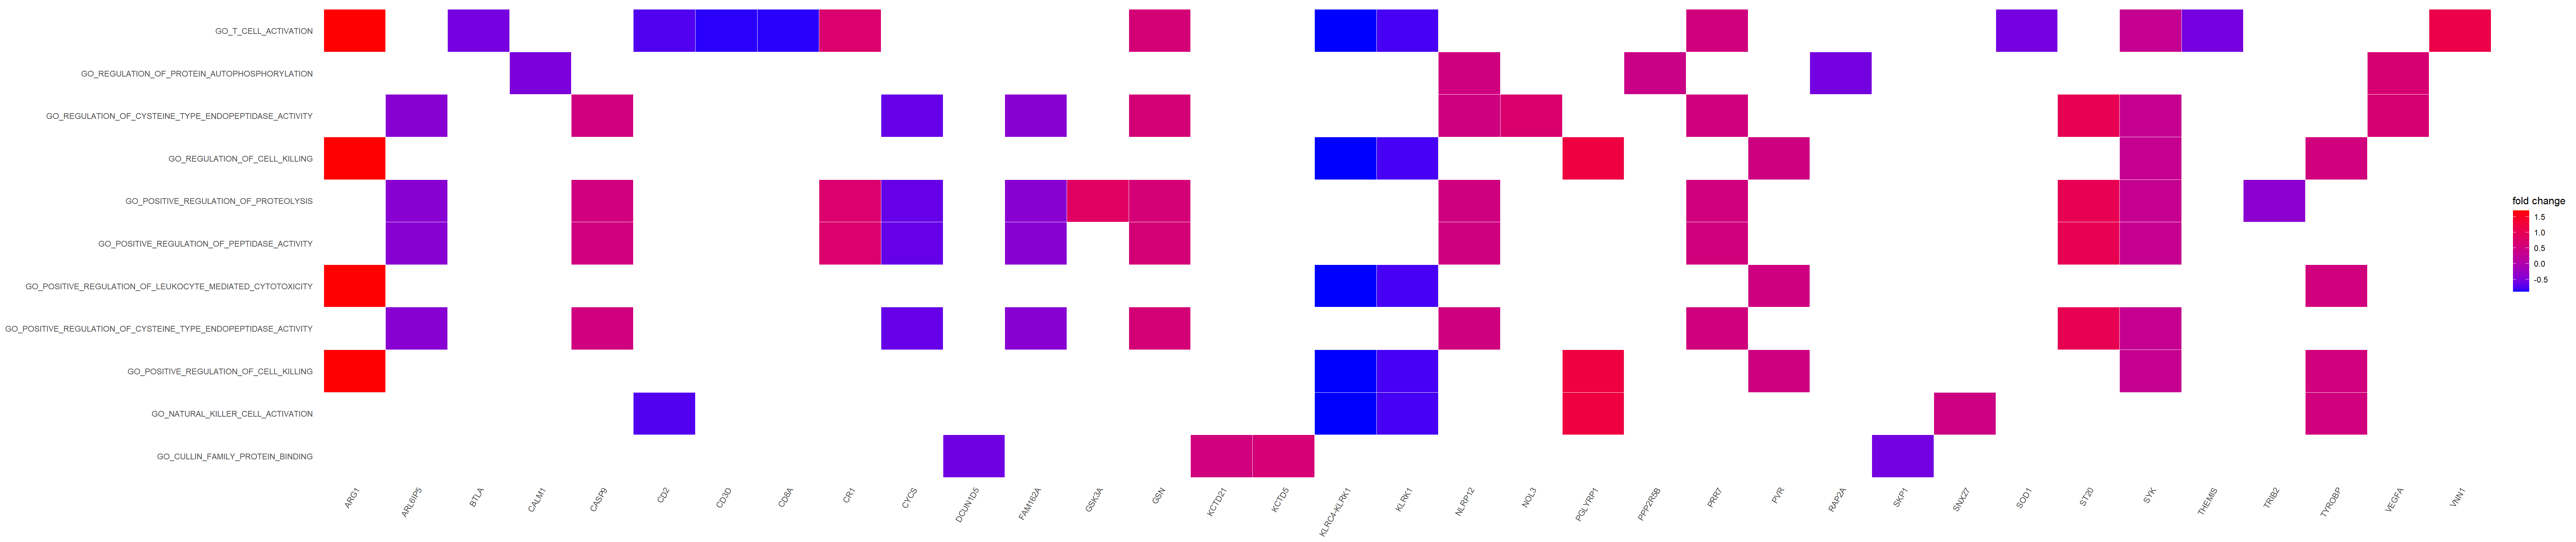
\includegraphics[width=10cm]{Figures/GSEA/CTLvs2bl_ef_heatmap.png} }}%
\caption{Functional analysis visualizations of Blood-HD-f-S2.}
\end{figure}

% HD-Blood-f-S3
\begin{figure}[!ht]%
    \centering
    \subfloat[\centering Enrichment map for ORA. ]{{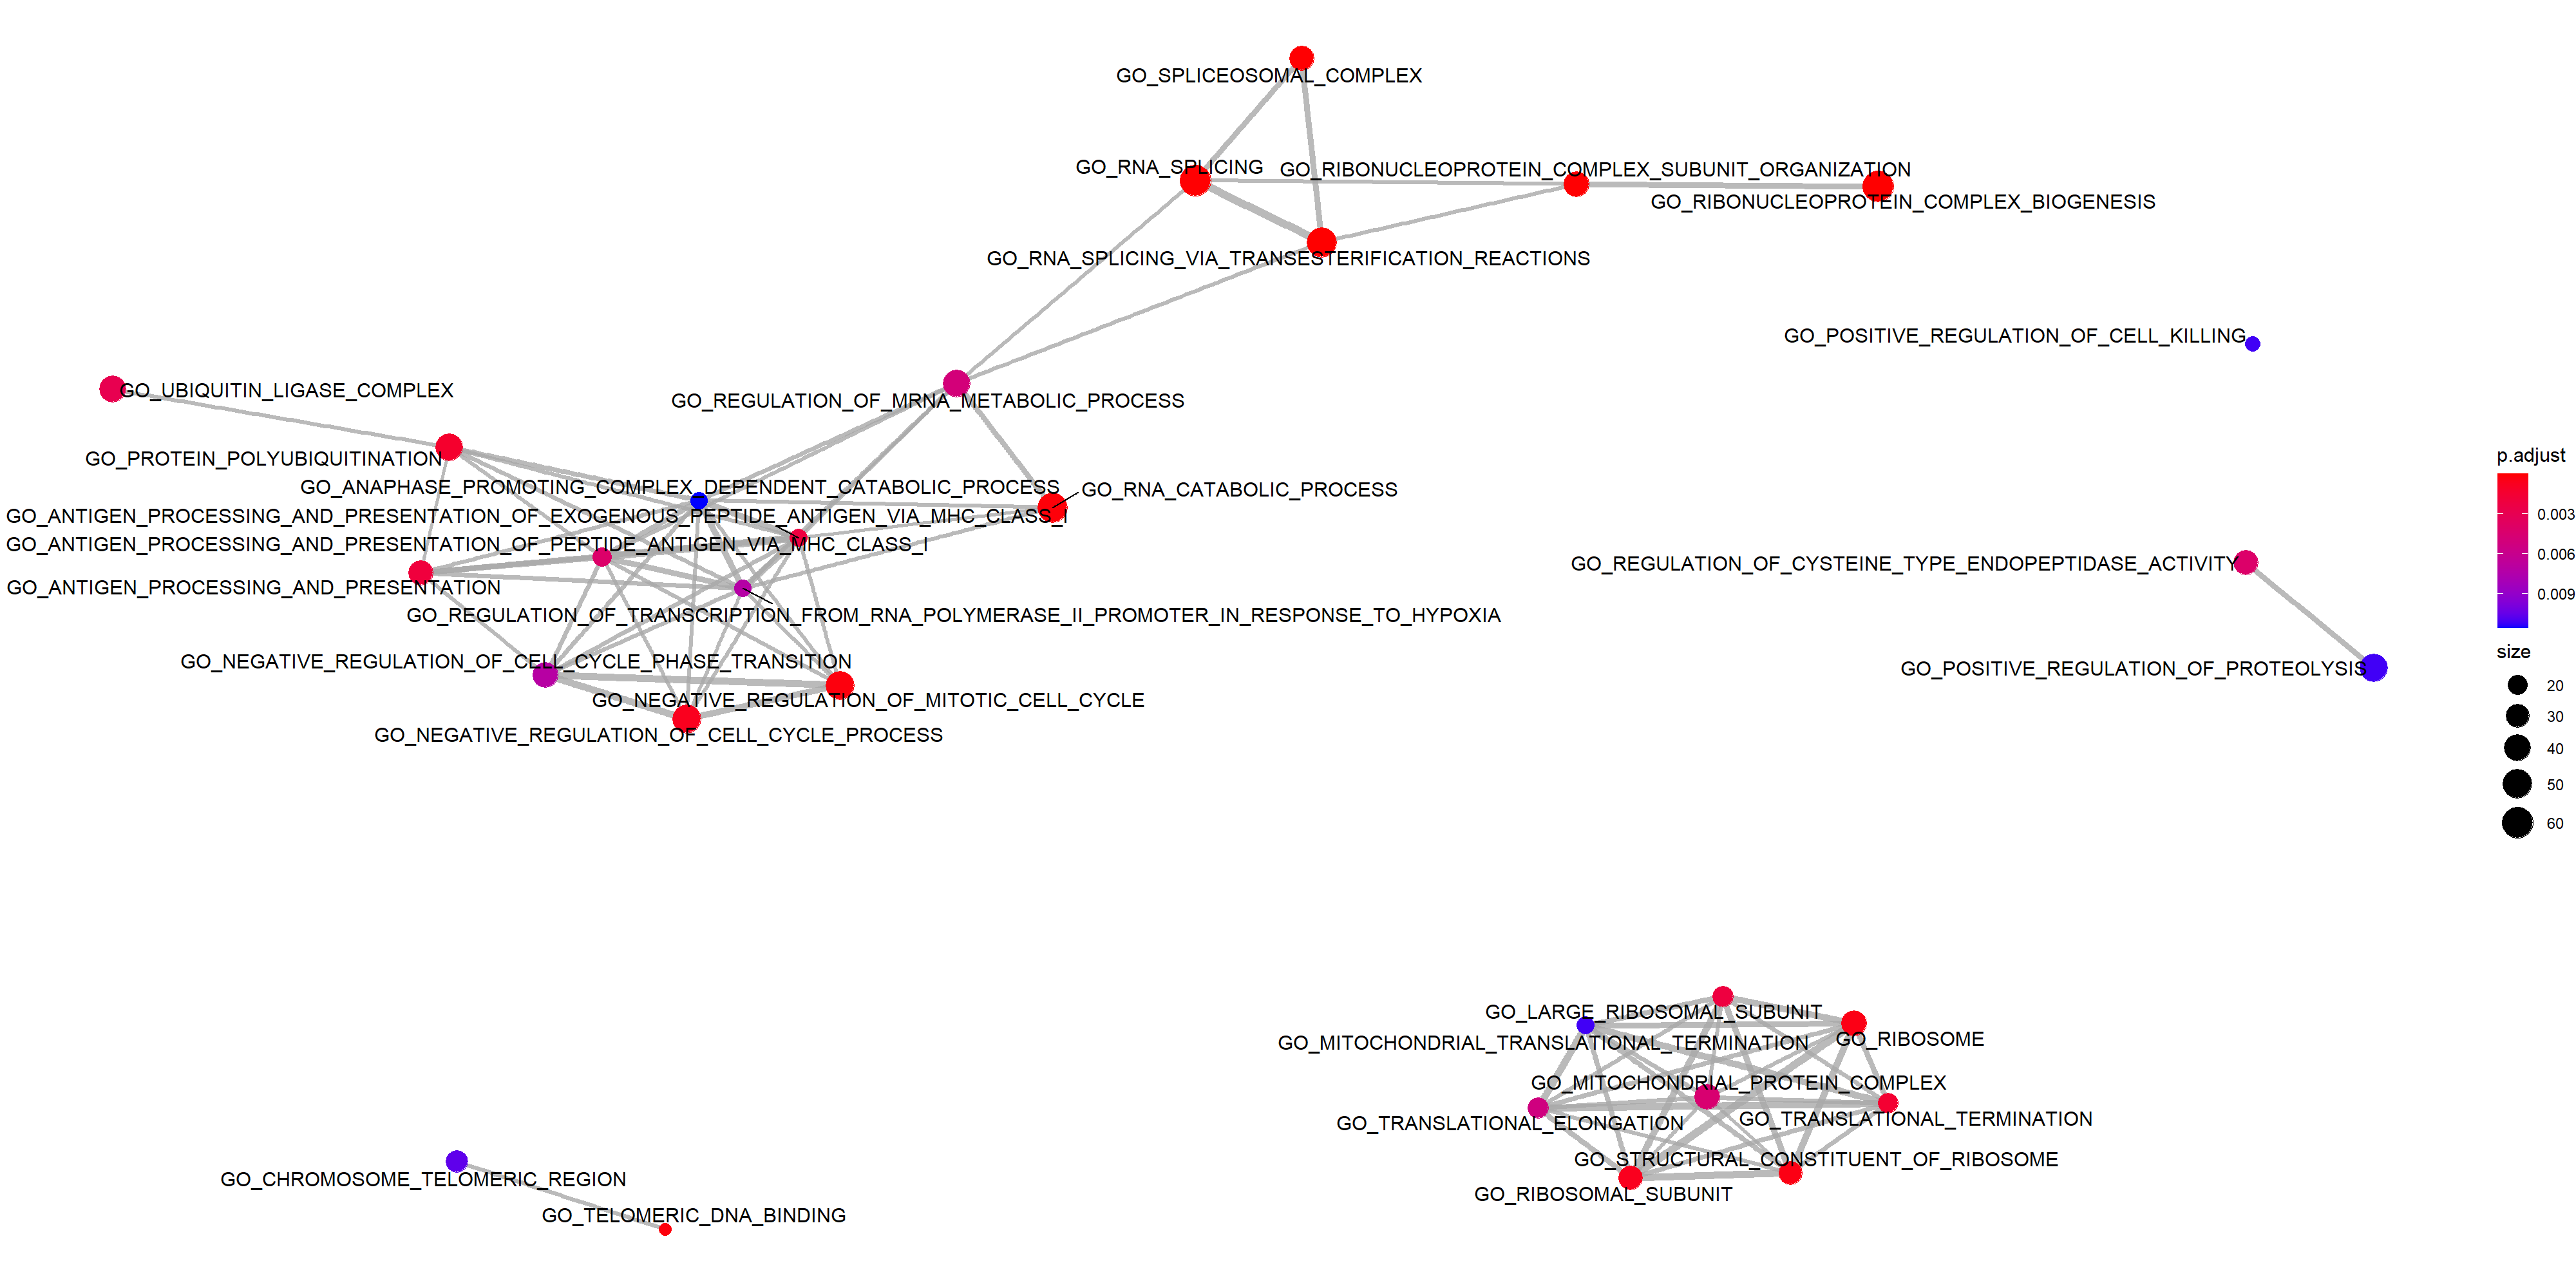
\includegraphics[width=10cm]{Figures/GSEA/CTLvs3bl_ef_emapplot.png} }}%
    \\
    \subfloat[\centering Gene-concept network for ORA. ]{{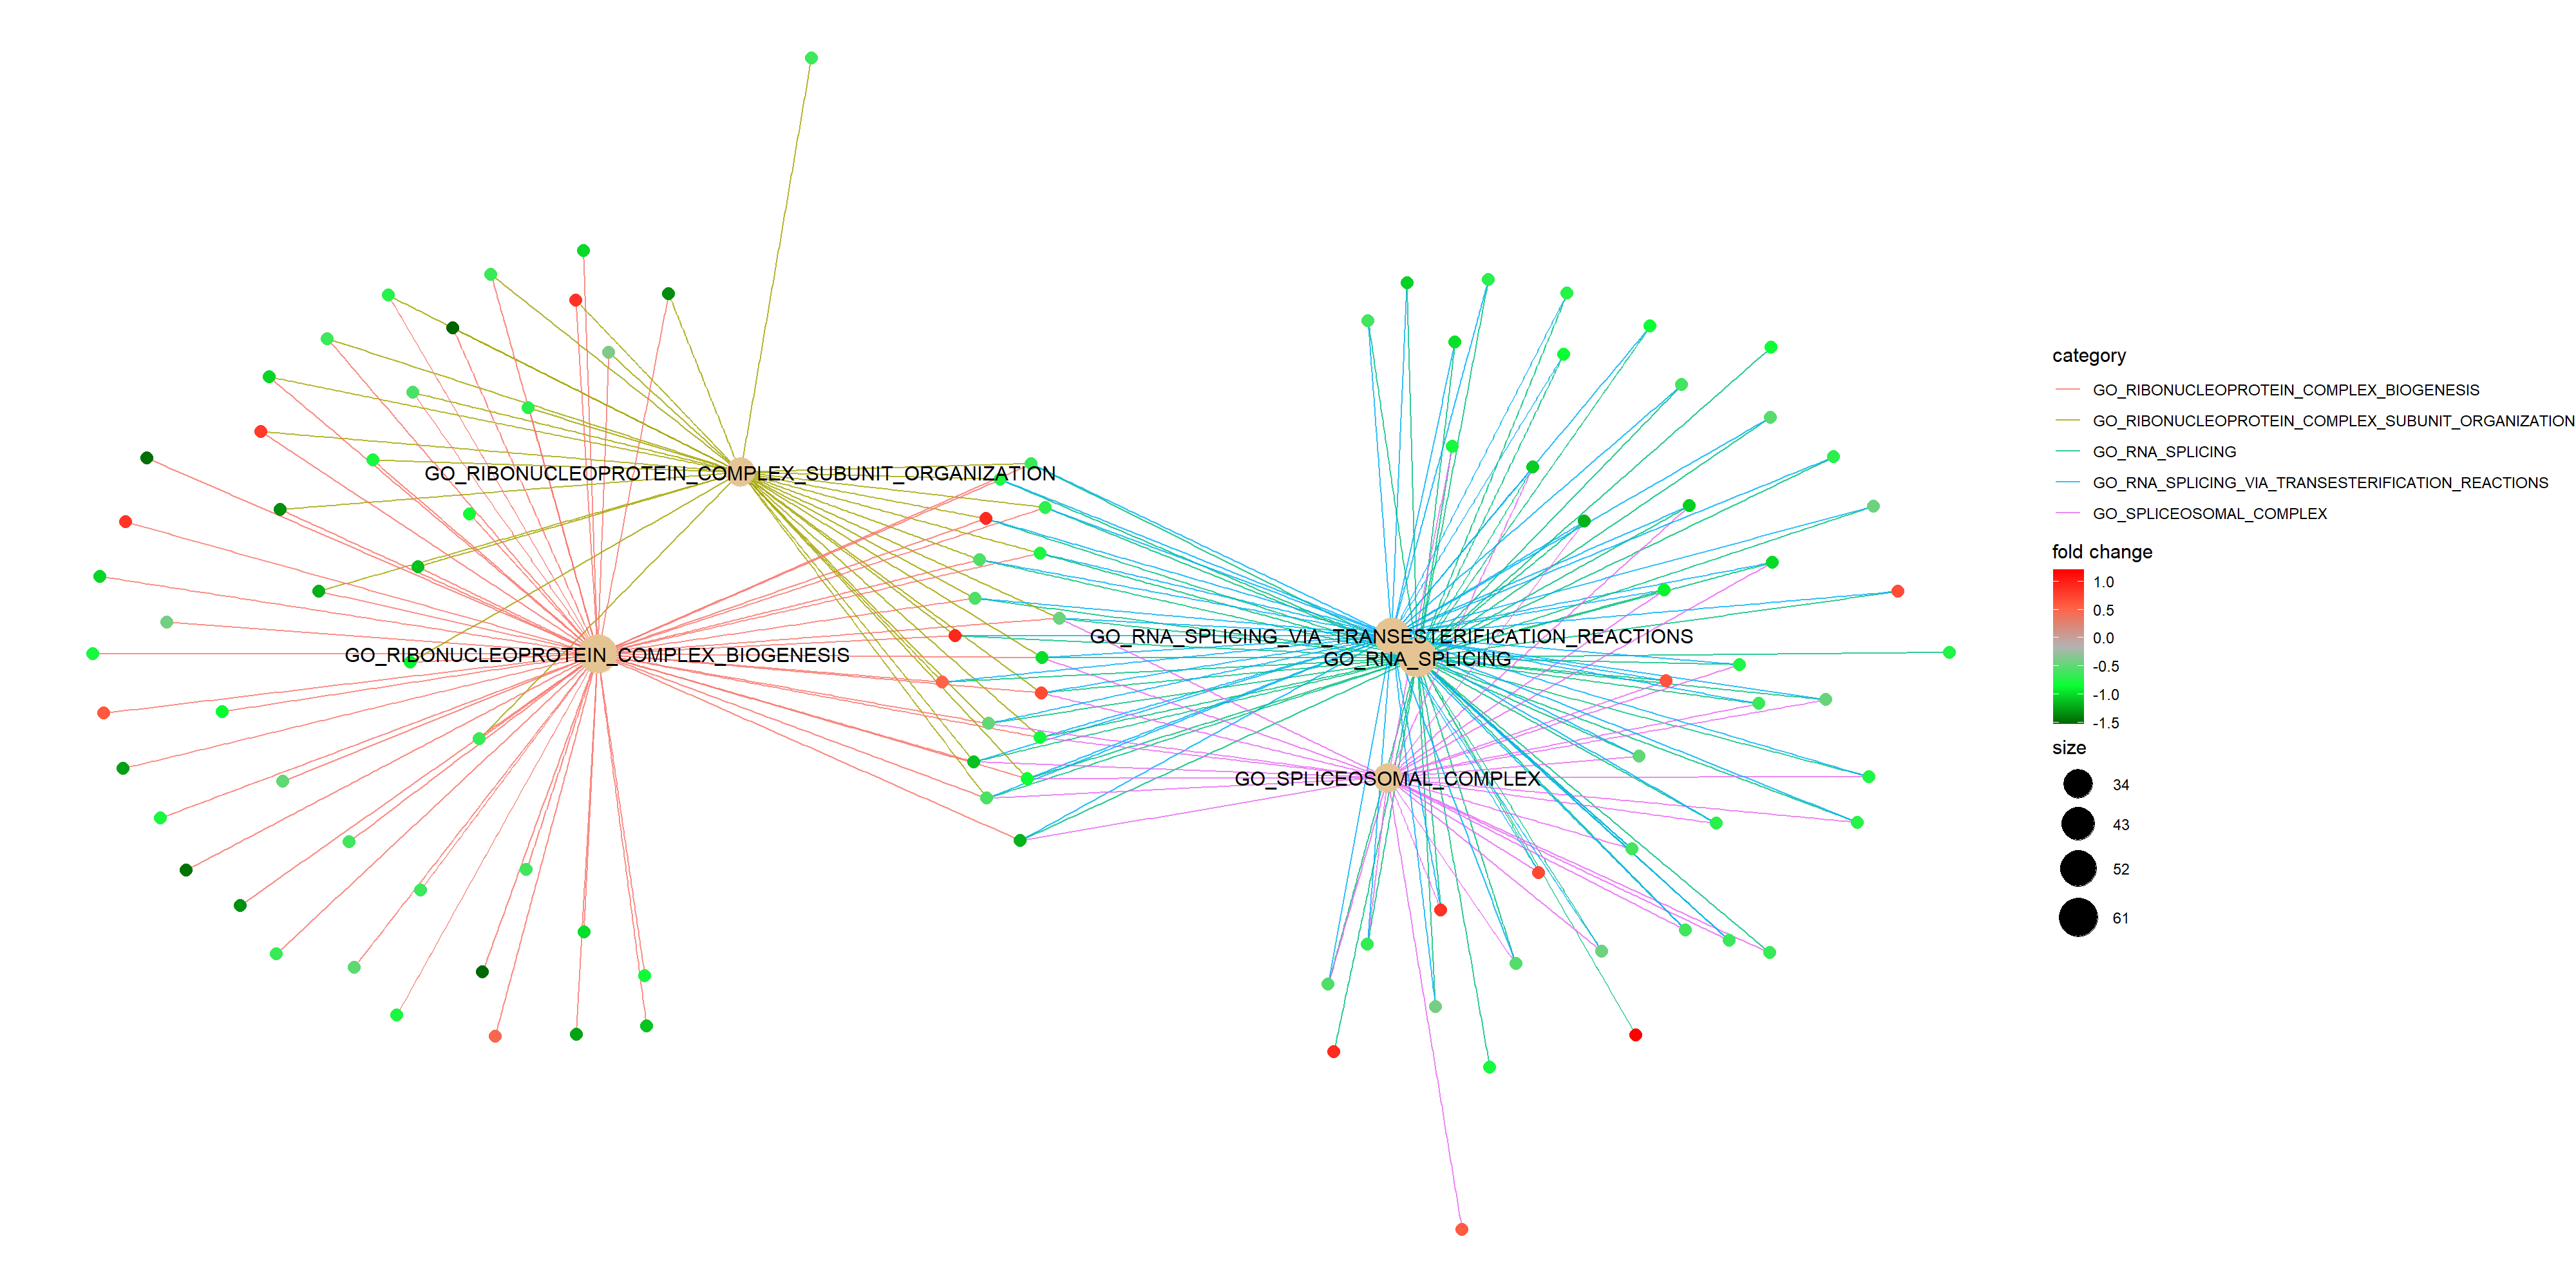
\includegraphics[width=10cm]{Figures/GSEA/CTLvs3bl_ef_cnetplot.png} }}%
    \\
    \subfloat[\centering Heatmap for ORA. ]{{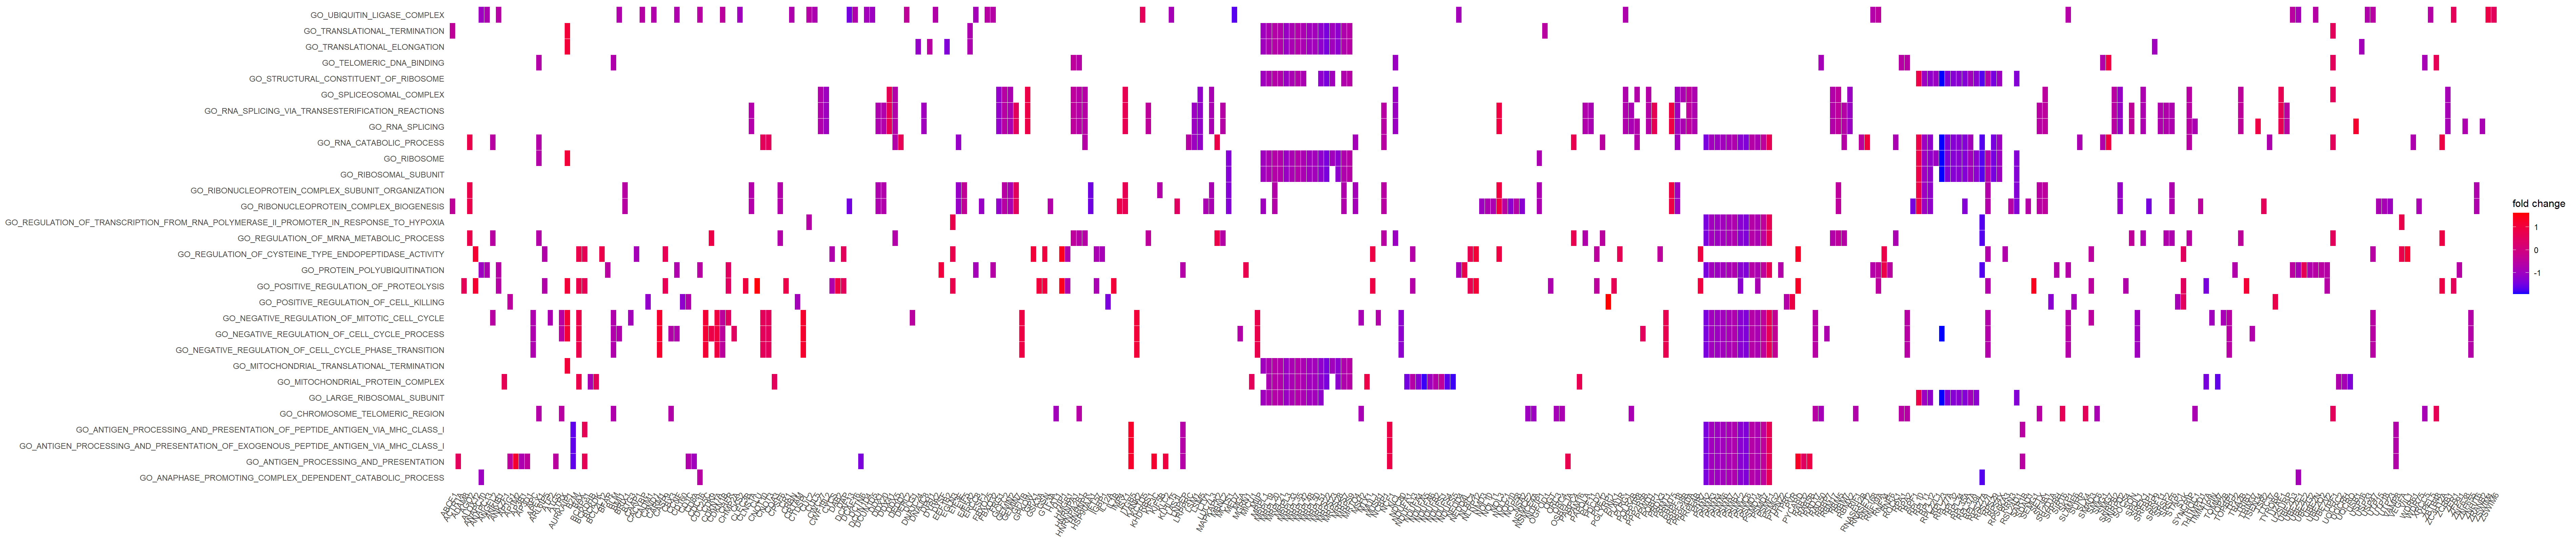
\includegraphics[width=10cm]{Figures/GSEA/CTLvs3bl_ef_heatmap.png} }}%
\caption{Functional analysis visualizations of Blood-HD-f-S3.}
\end{figure}

% HD-Blood-m
\begin{figure}[!ht]%
    \centering
    \subfloat[\centering Enrichment map for ORA. ]{{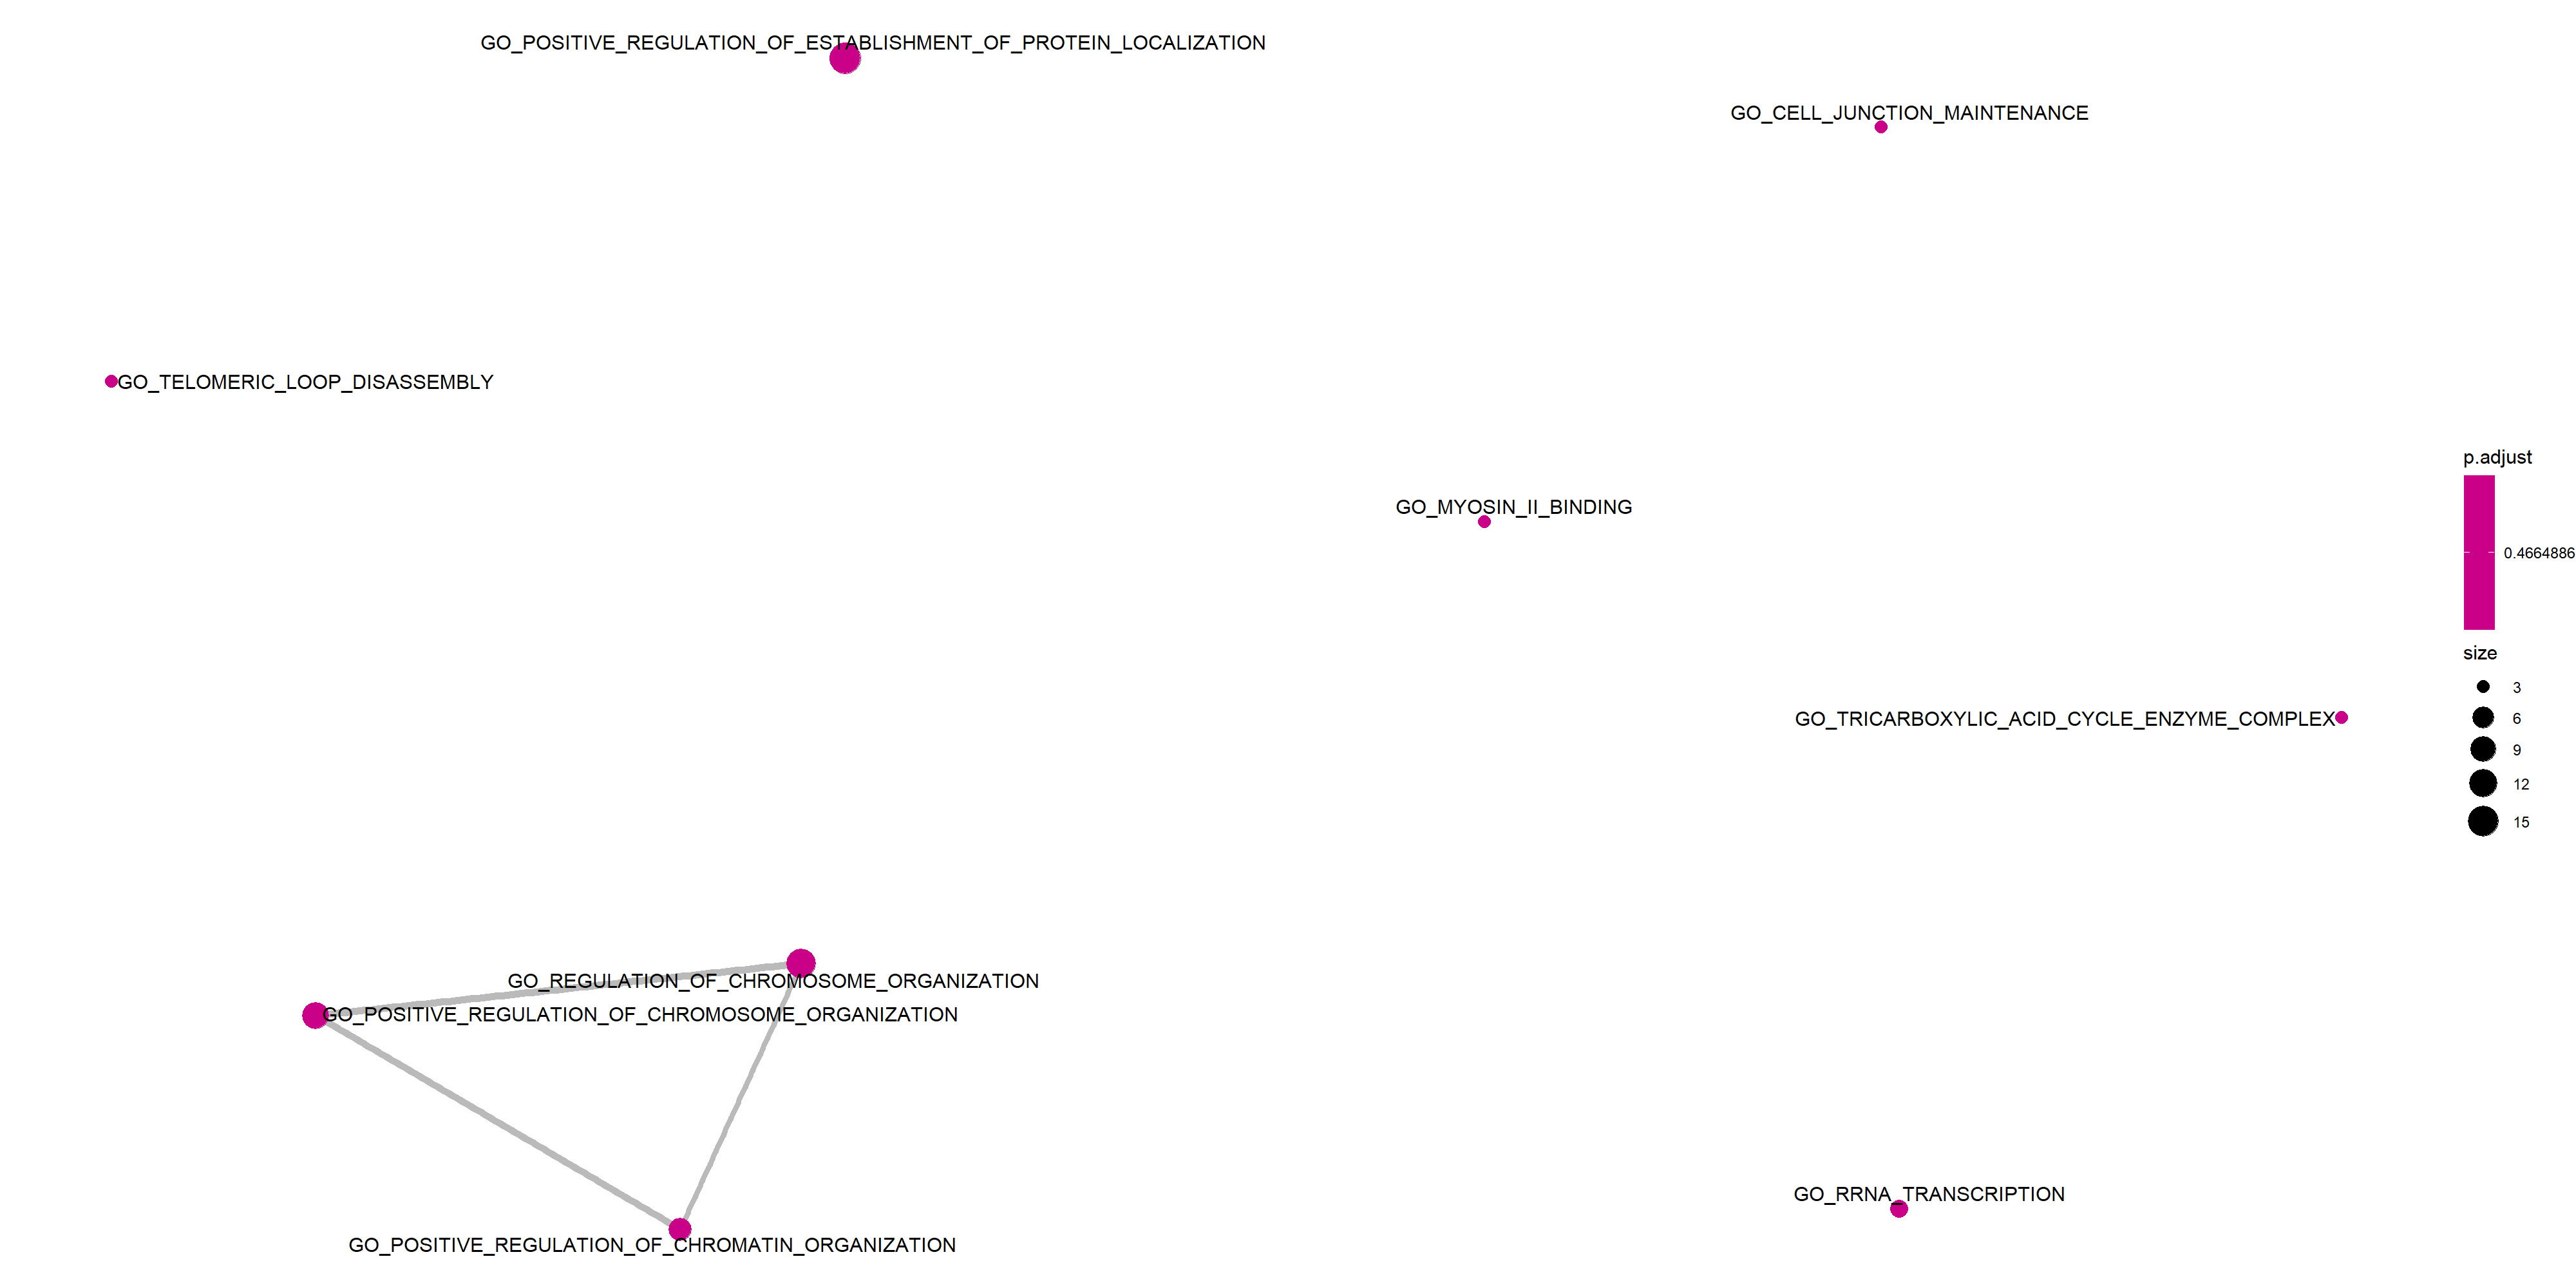
\includegraphics[width=10cm]{Figures/GSEA/CTLvsHD_em_emapplot.png} }}%
    \\
    \subfloat[\centering Gene-concept network for ORA. ]{{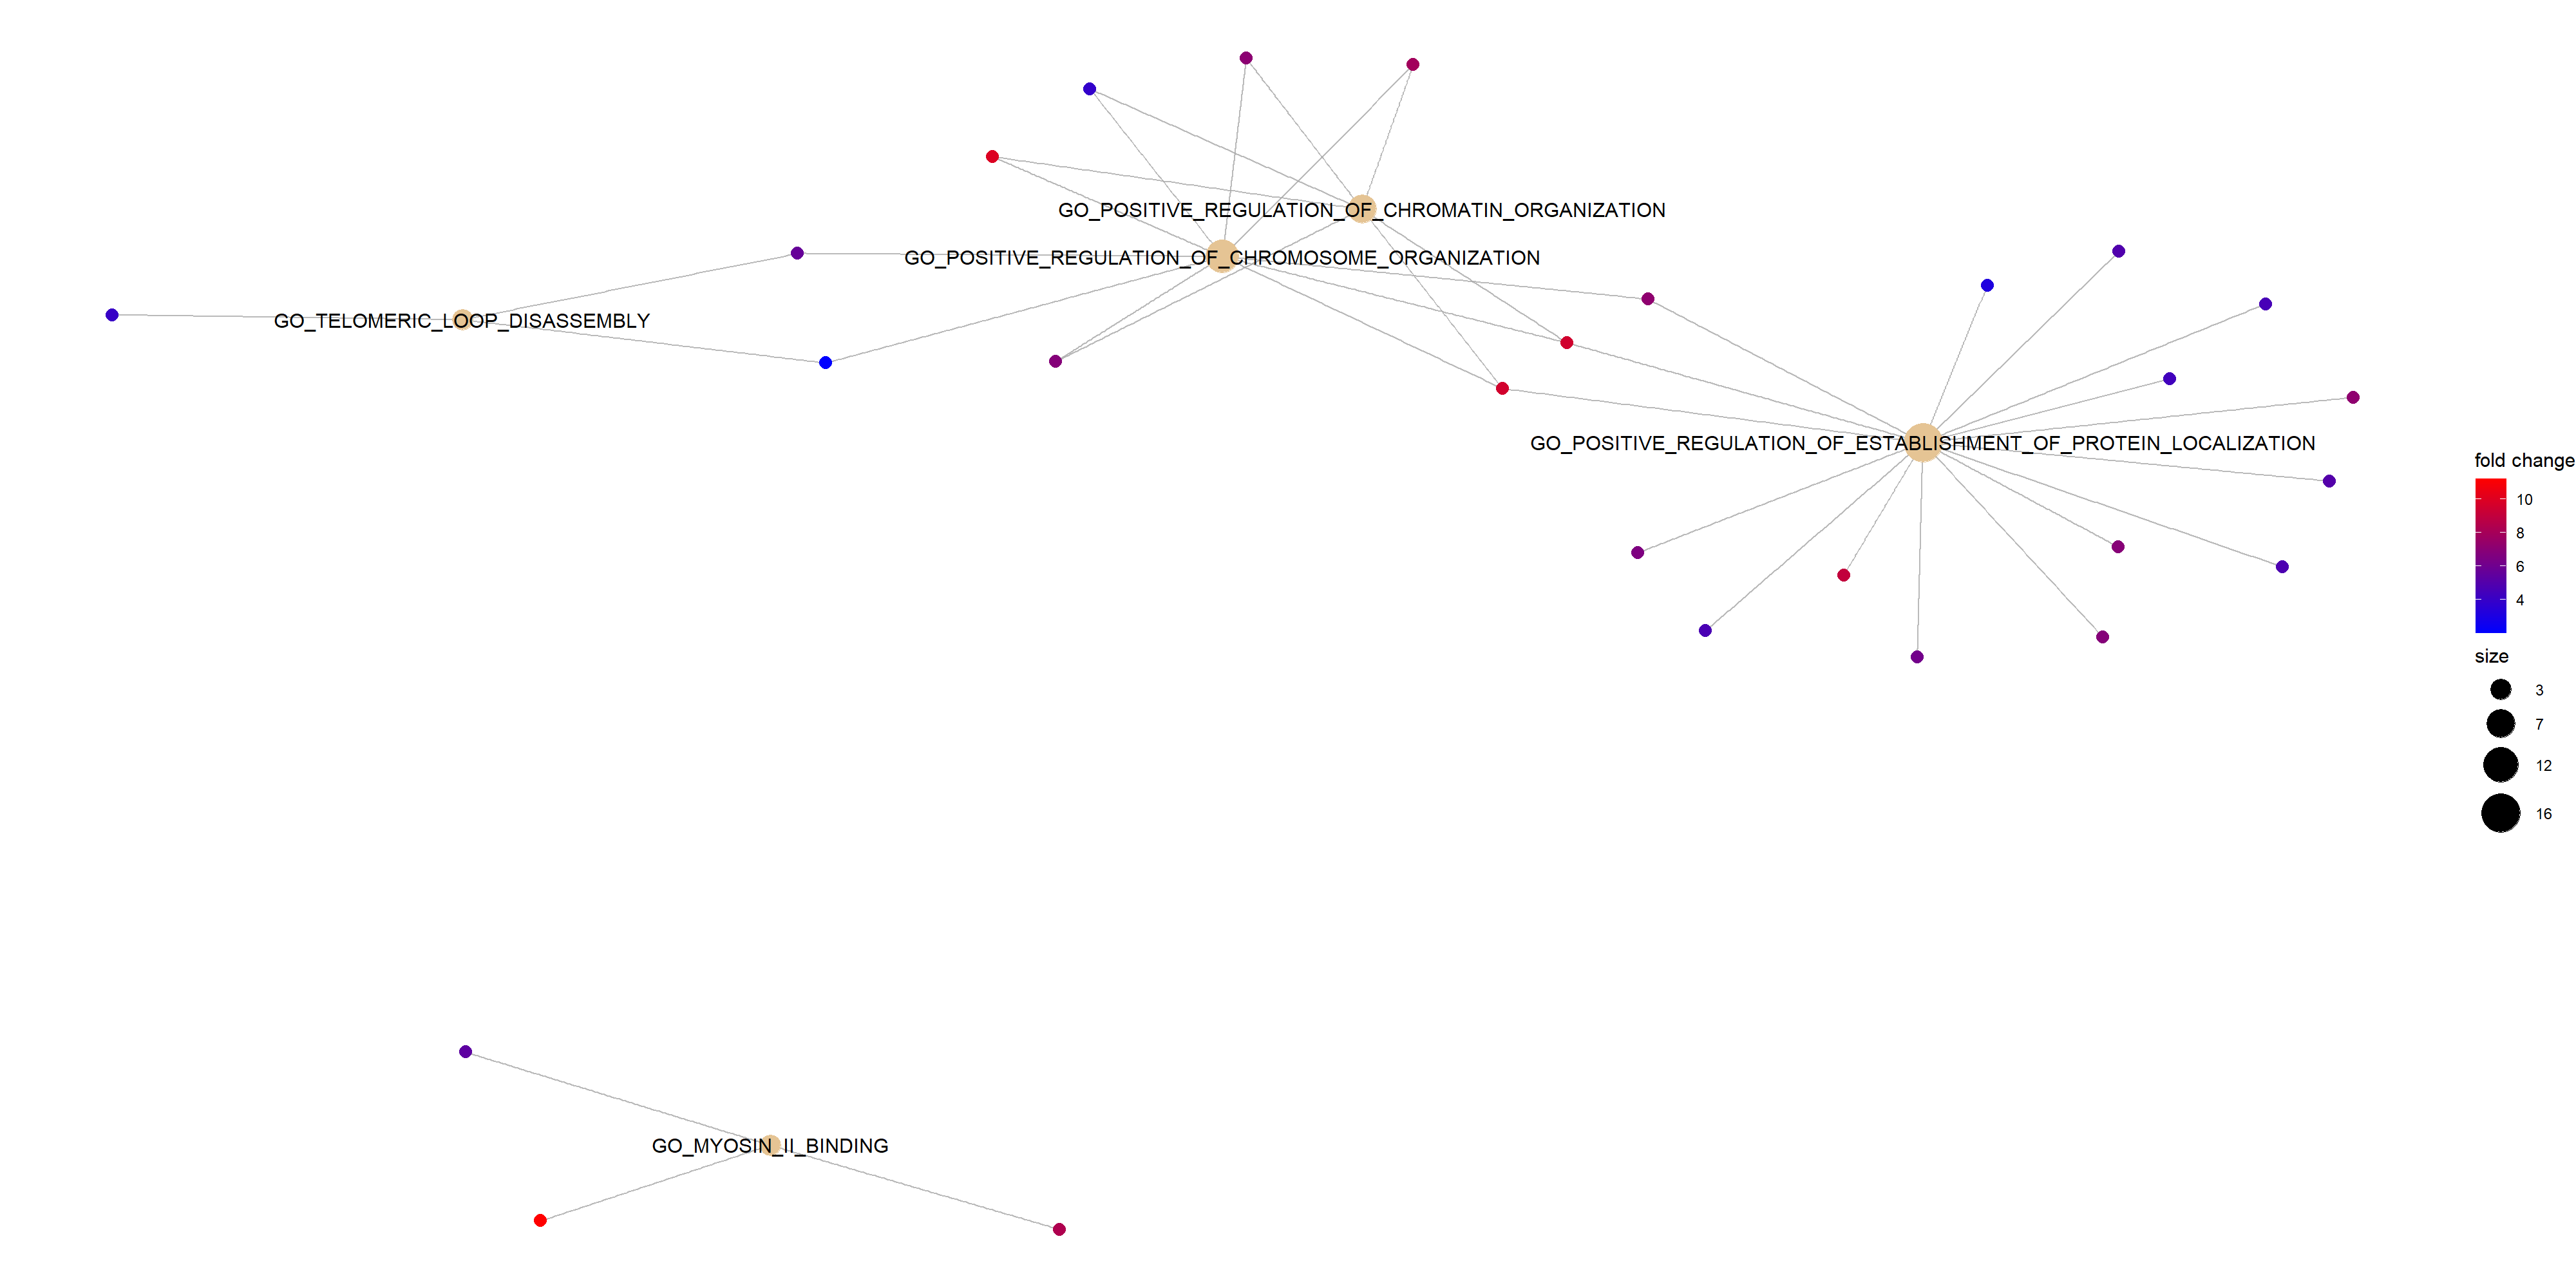
\includegraphics[width=10cm]{Figures/GSEA/CTLvsHD_em_cnetplot.png} }}%
    \\
    \subfloat[\centering Heatmap for ORA. ]{{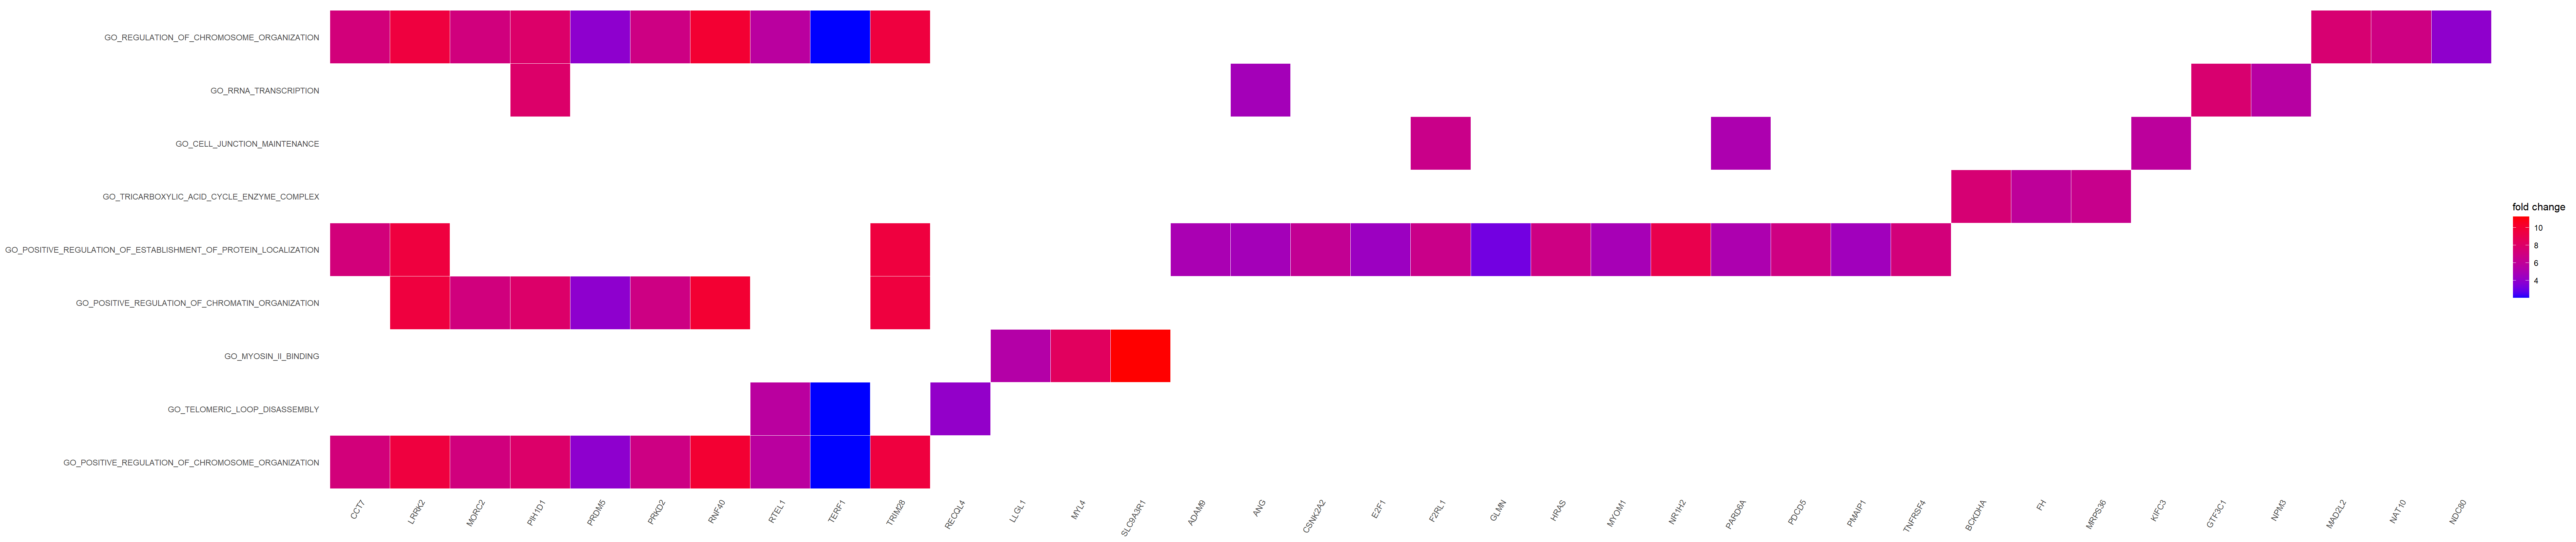
\includegraphics[width=10cm]{Figures/GSEA/CTLvsHD_em_heatmap.png} }}%
\caption{Functional analysis visualizations of Blood-HD-m.}
\end{figure}

% HD-Blood-m-S1
\begin{figure}[!ht]%
    \centering
    \subfloat[\centering Enrichment map for ORA. ]{{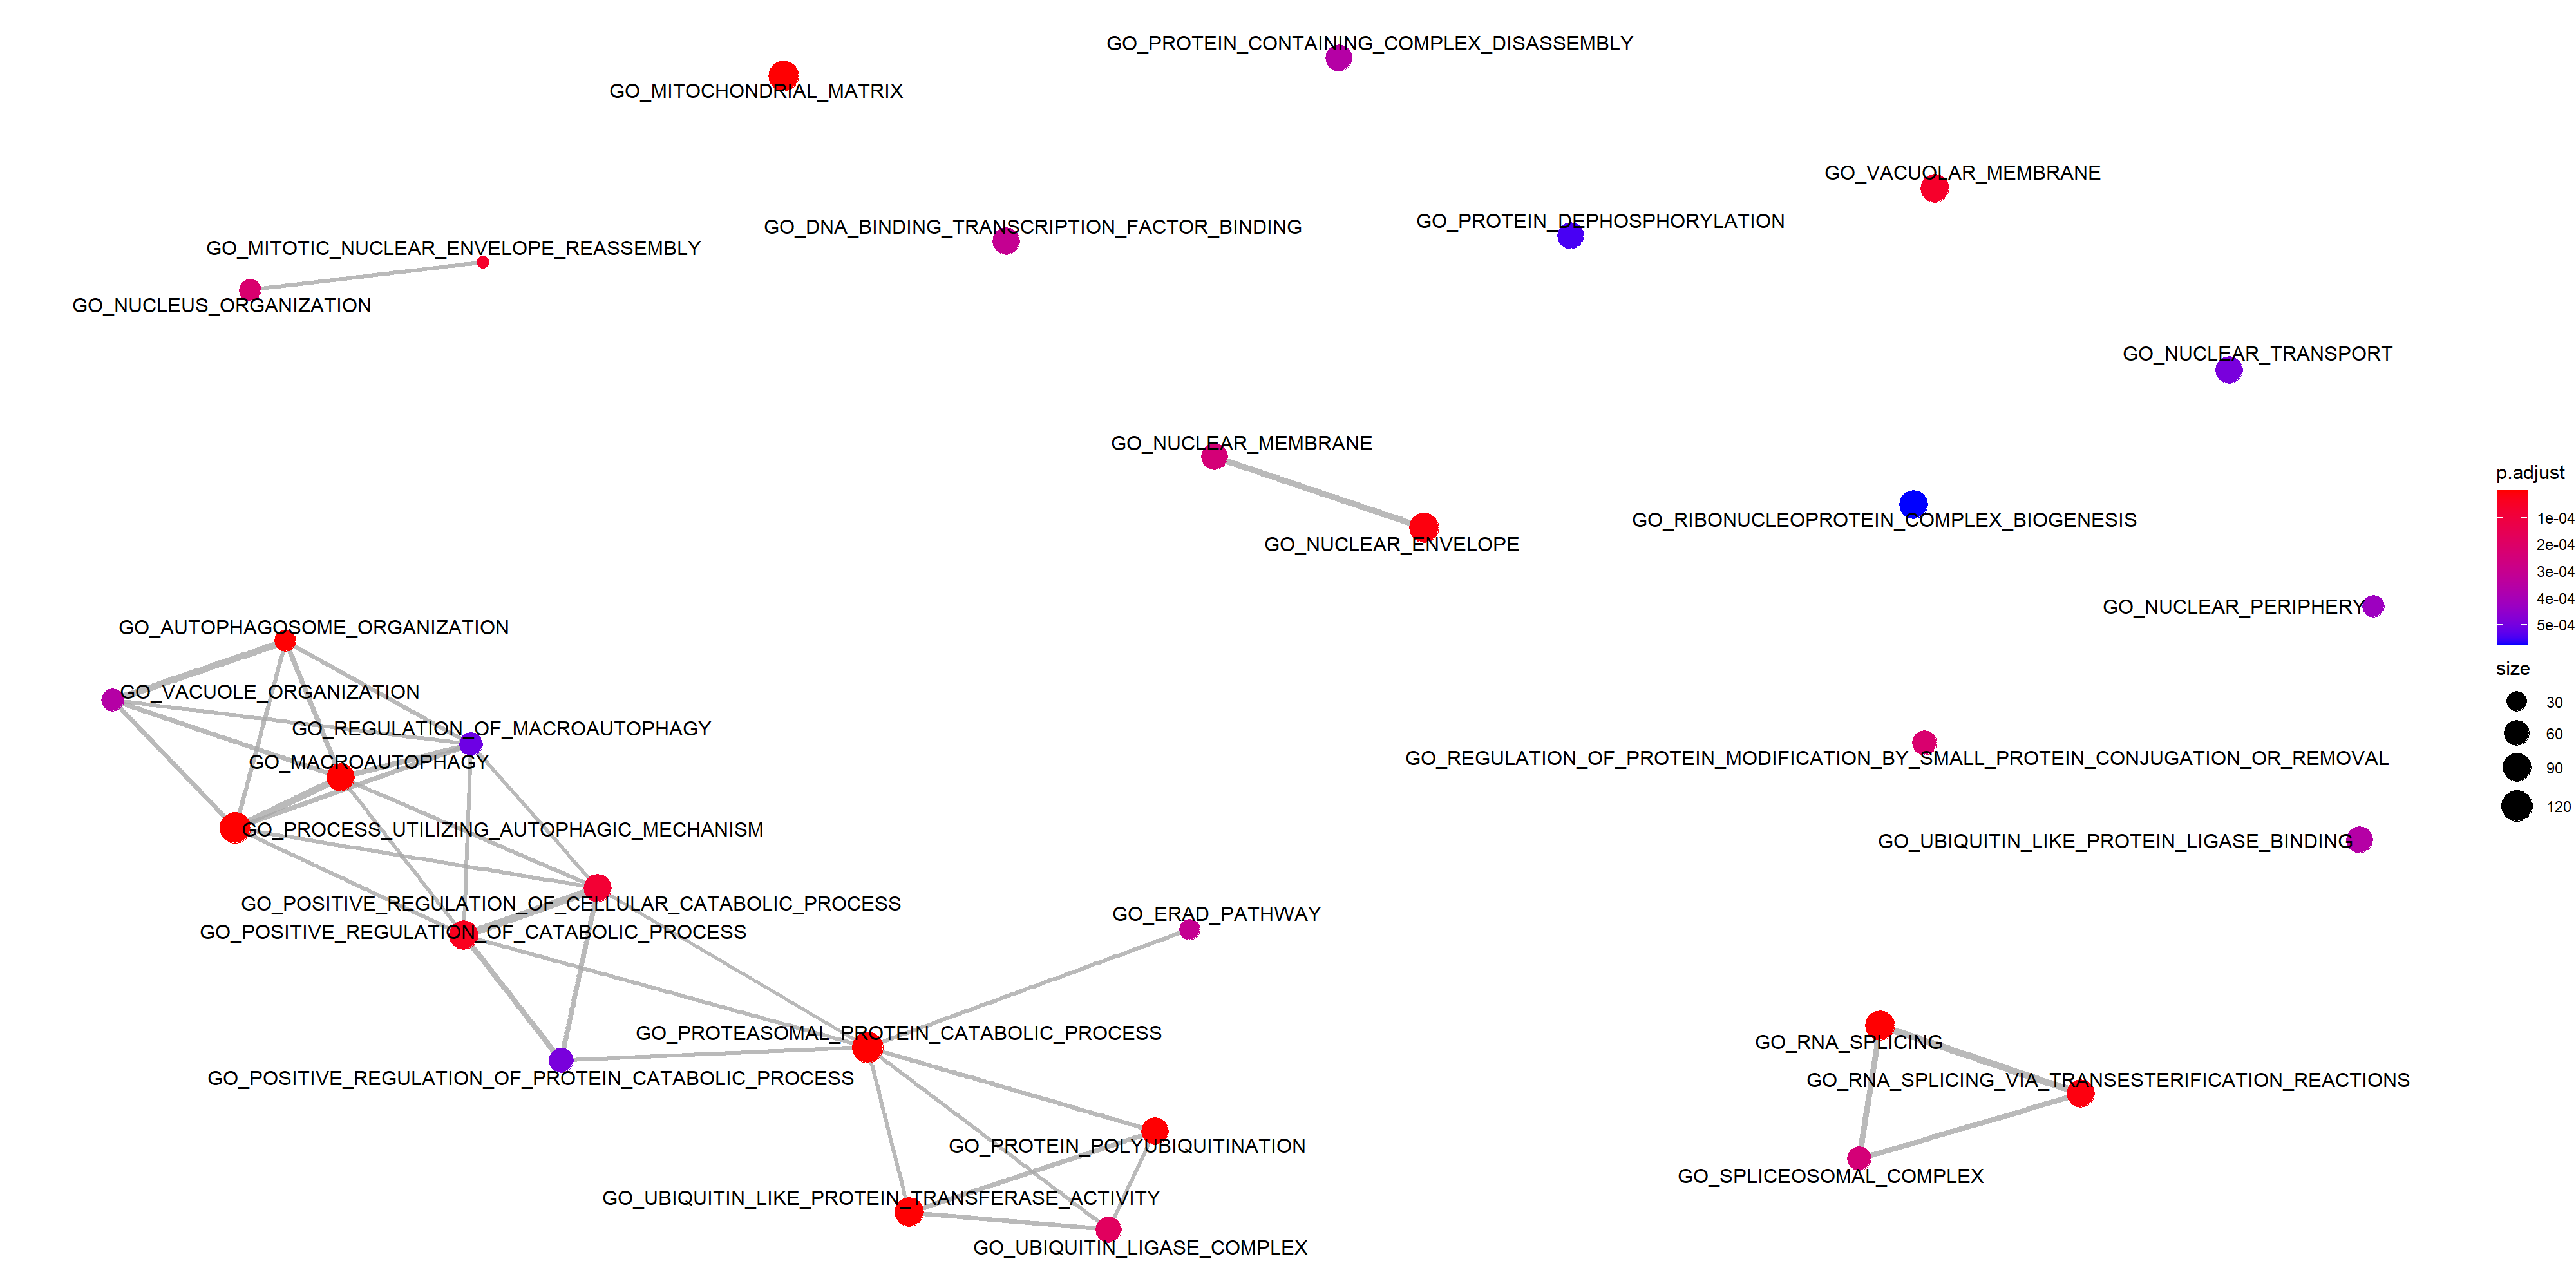
\includegraphics[width=10cm]{Figures/GSEA/CTLvs1bl_em_emapplot.png} }}%
    \\
    \subfloat[\centering Gene-concept network for ORA. ]{{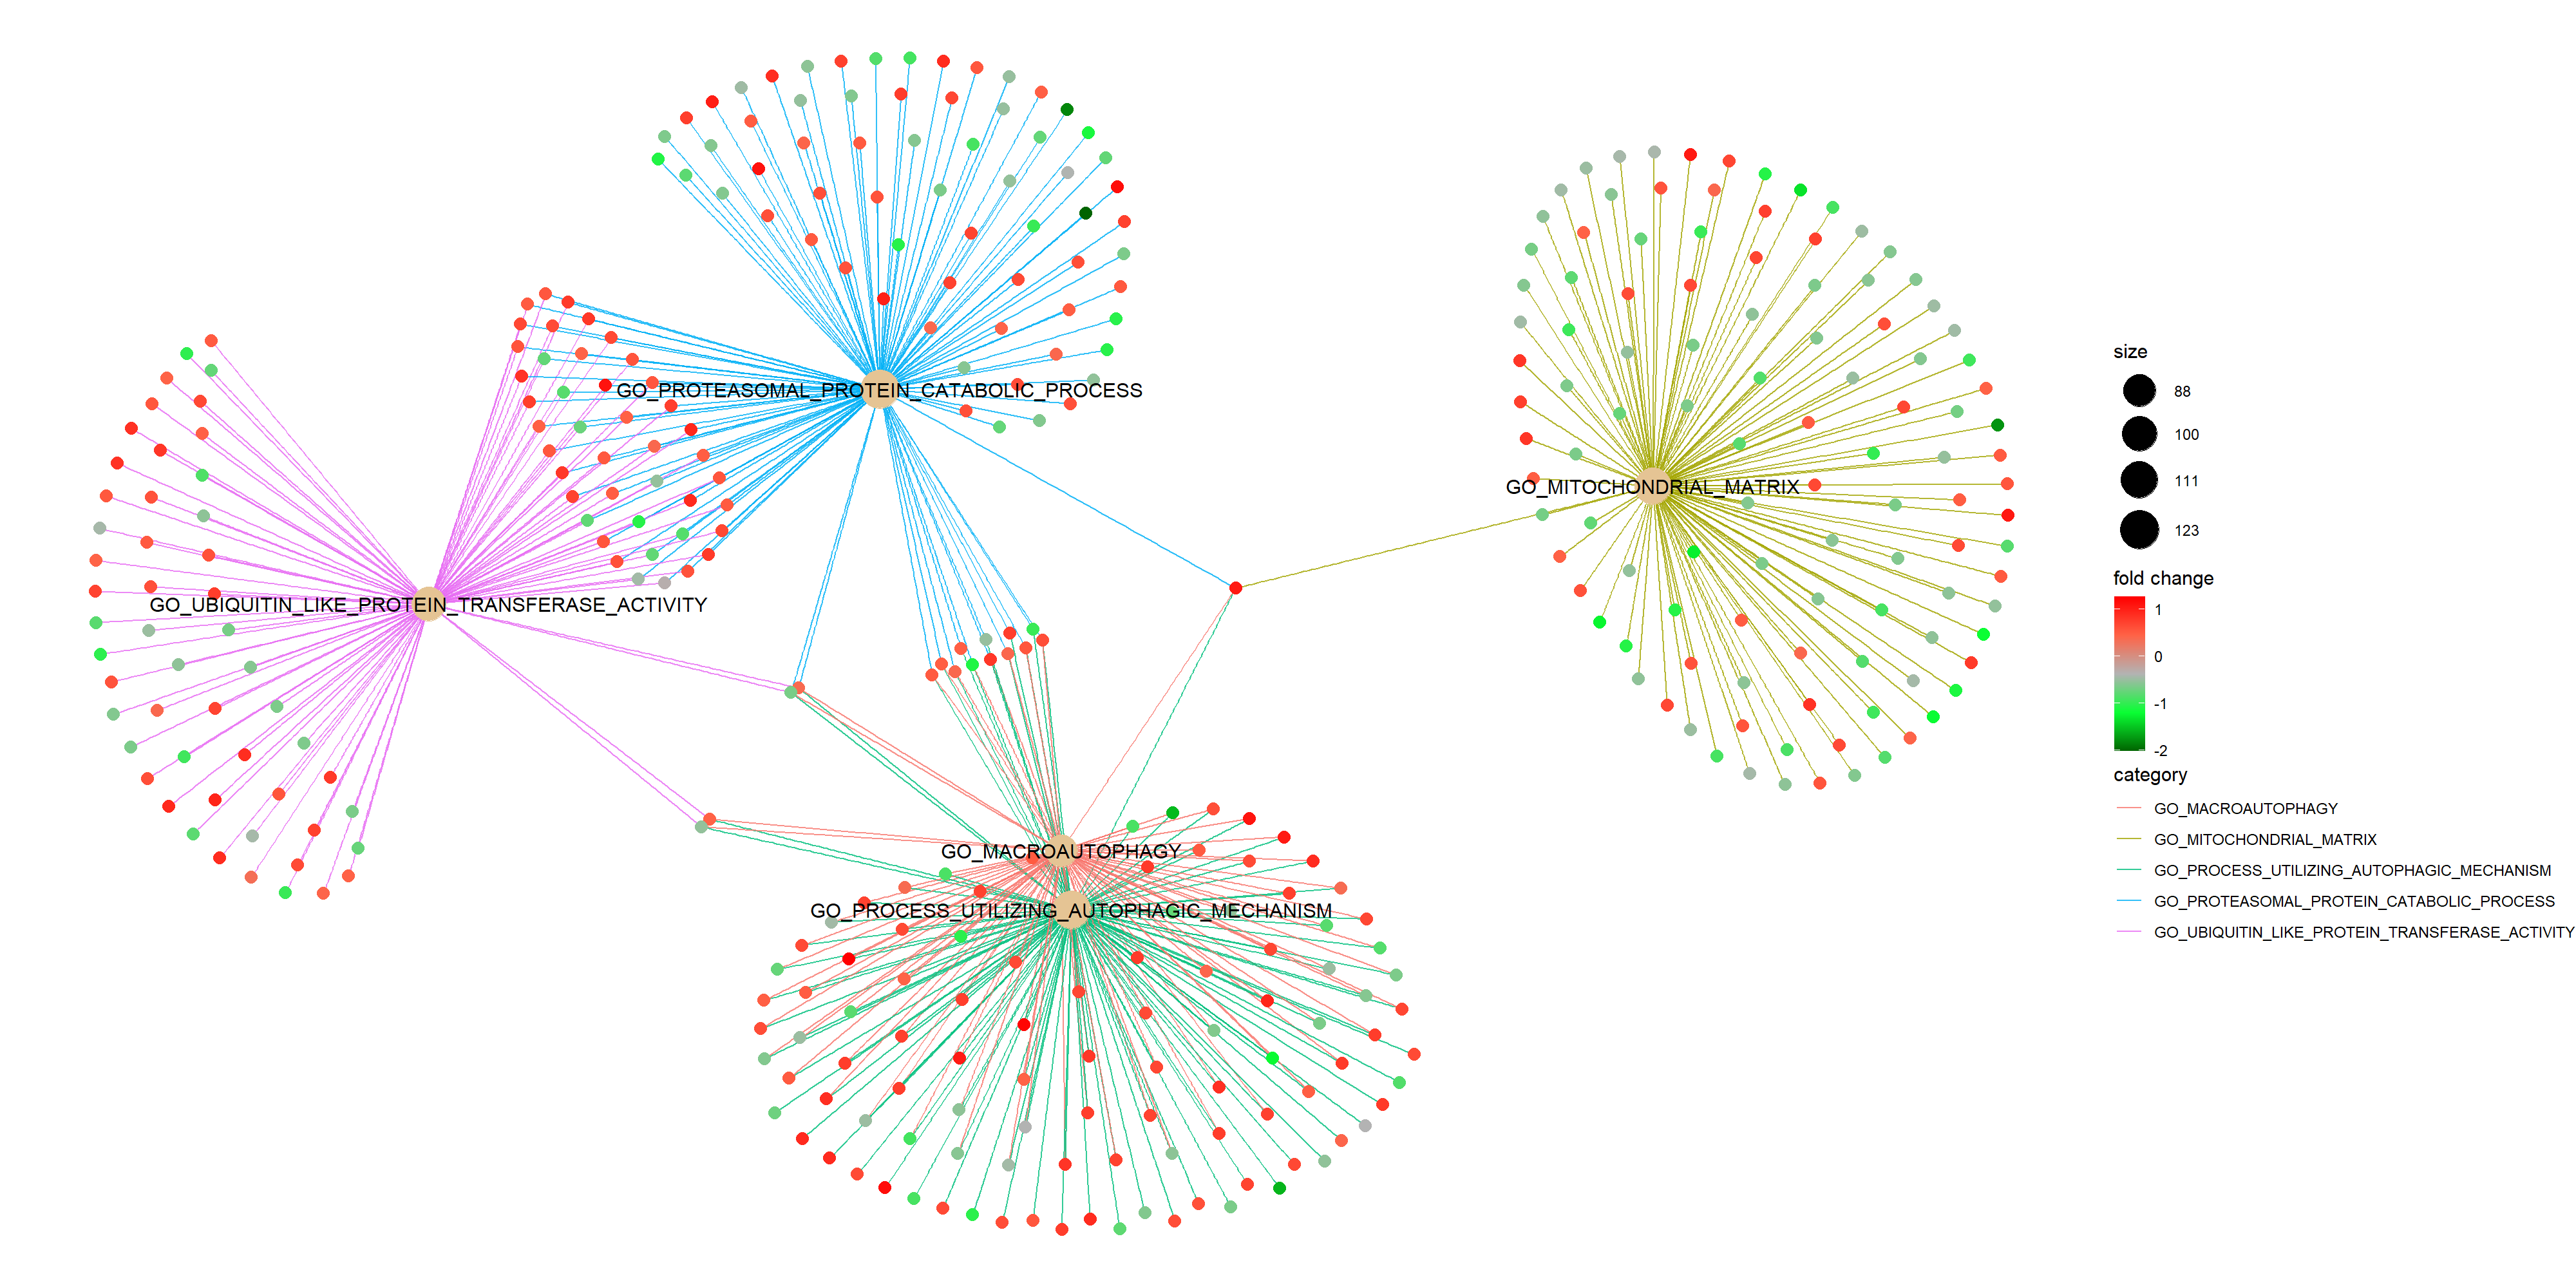
\includegraphics[width=10cm]{Figures/GSEA/CTLvs1bl_em_cnetplot.png} }}%
    \\
    \subfloat[\centering Heatmap for ORA. ]{{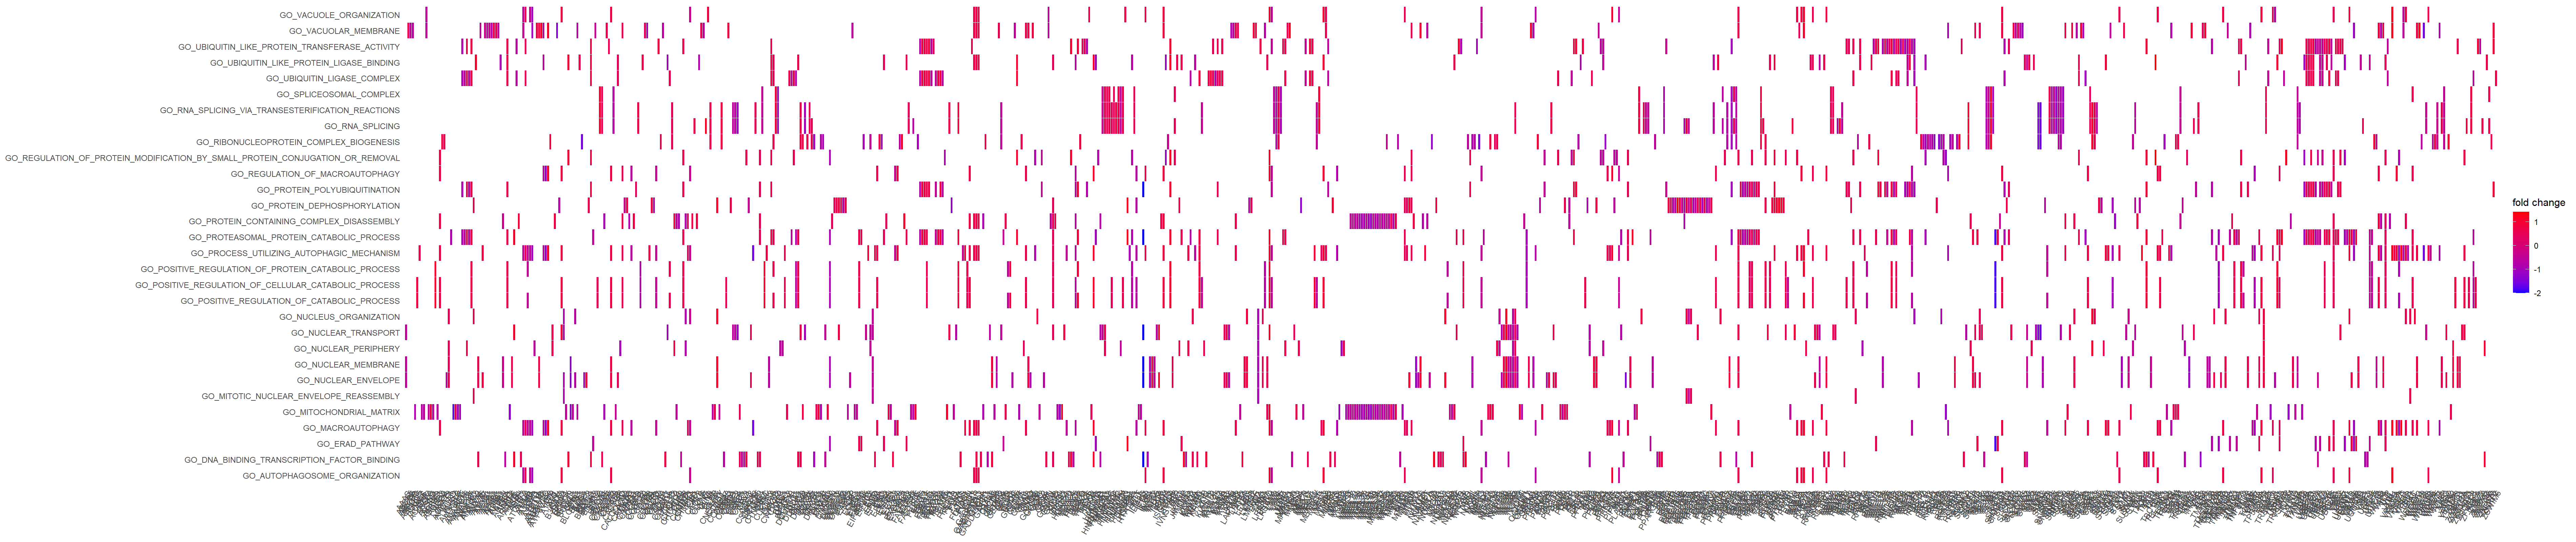
\includegraphics[width=10cm]{Figures/GSEA/CTLvs1bl_em_heatmap.png} }}%
\caption{Functional analysis visualizations of Blood-HD-m-S1.}
\end{figure}

% HD-Blood-m-S2
\begin{figure}[!ht]%
    \centering
    \subfloat[\centering Enrichment map for ORA. ]{{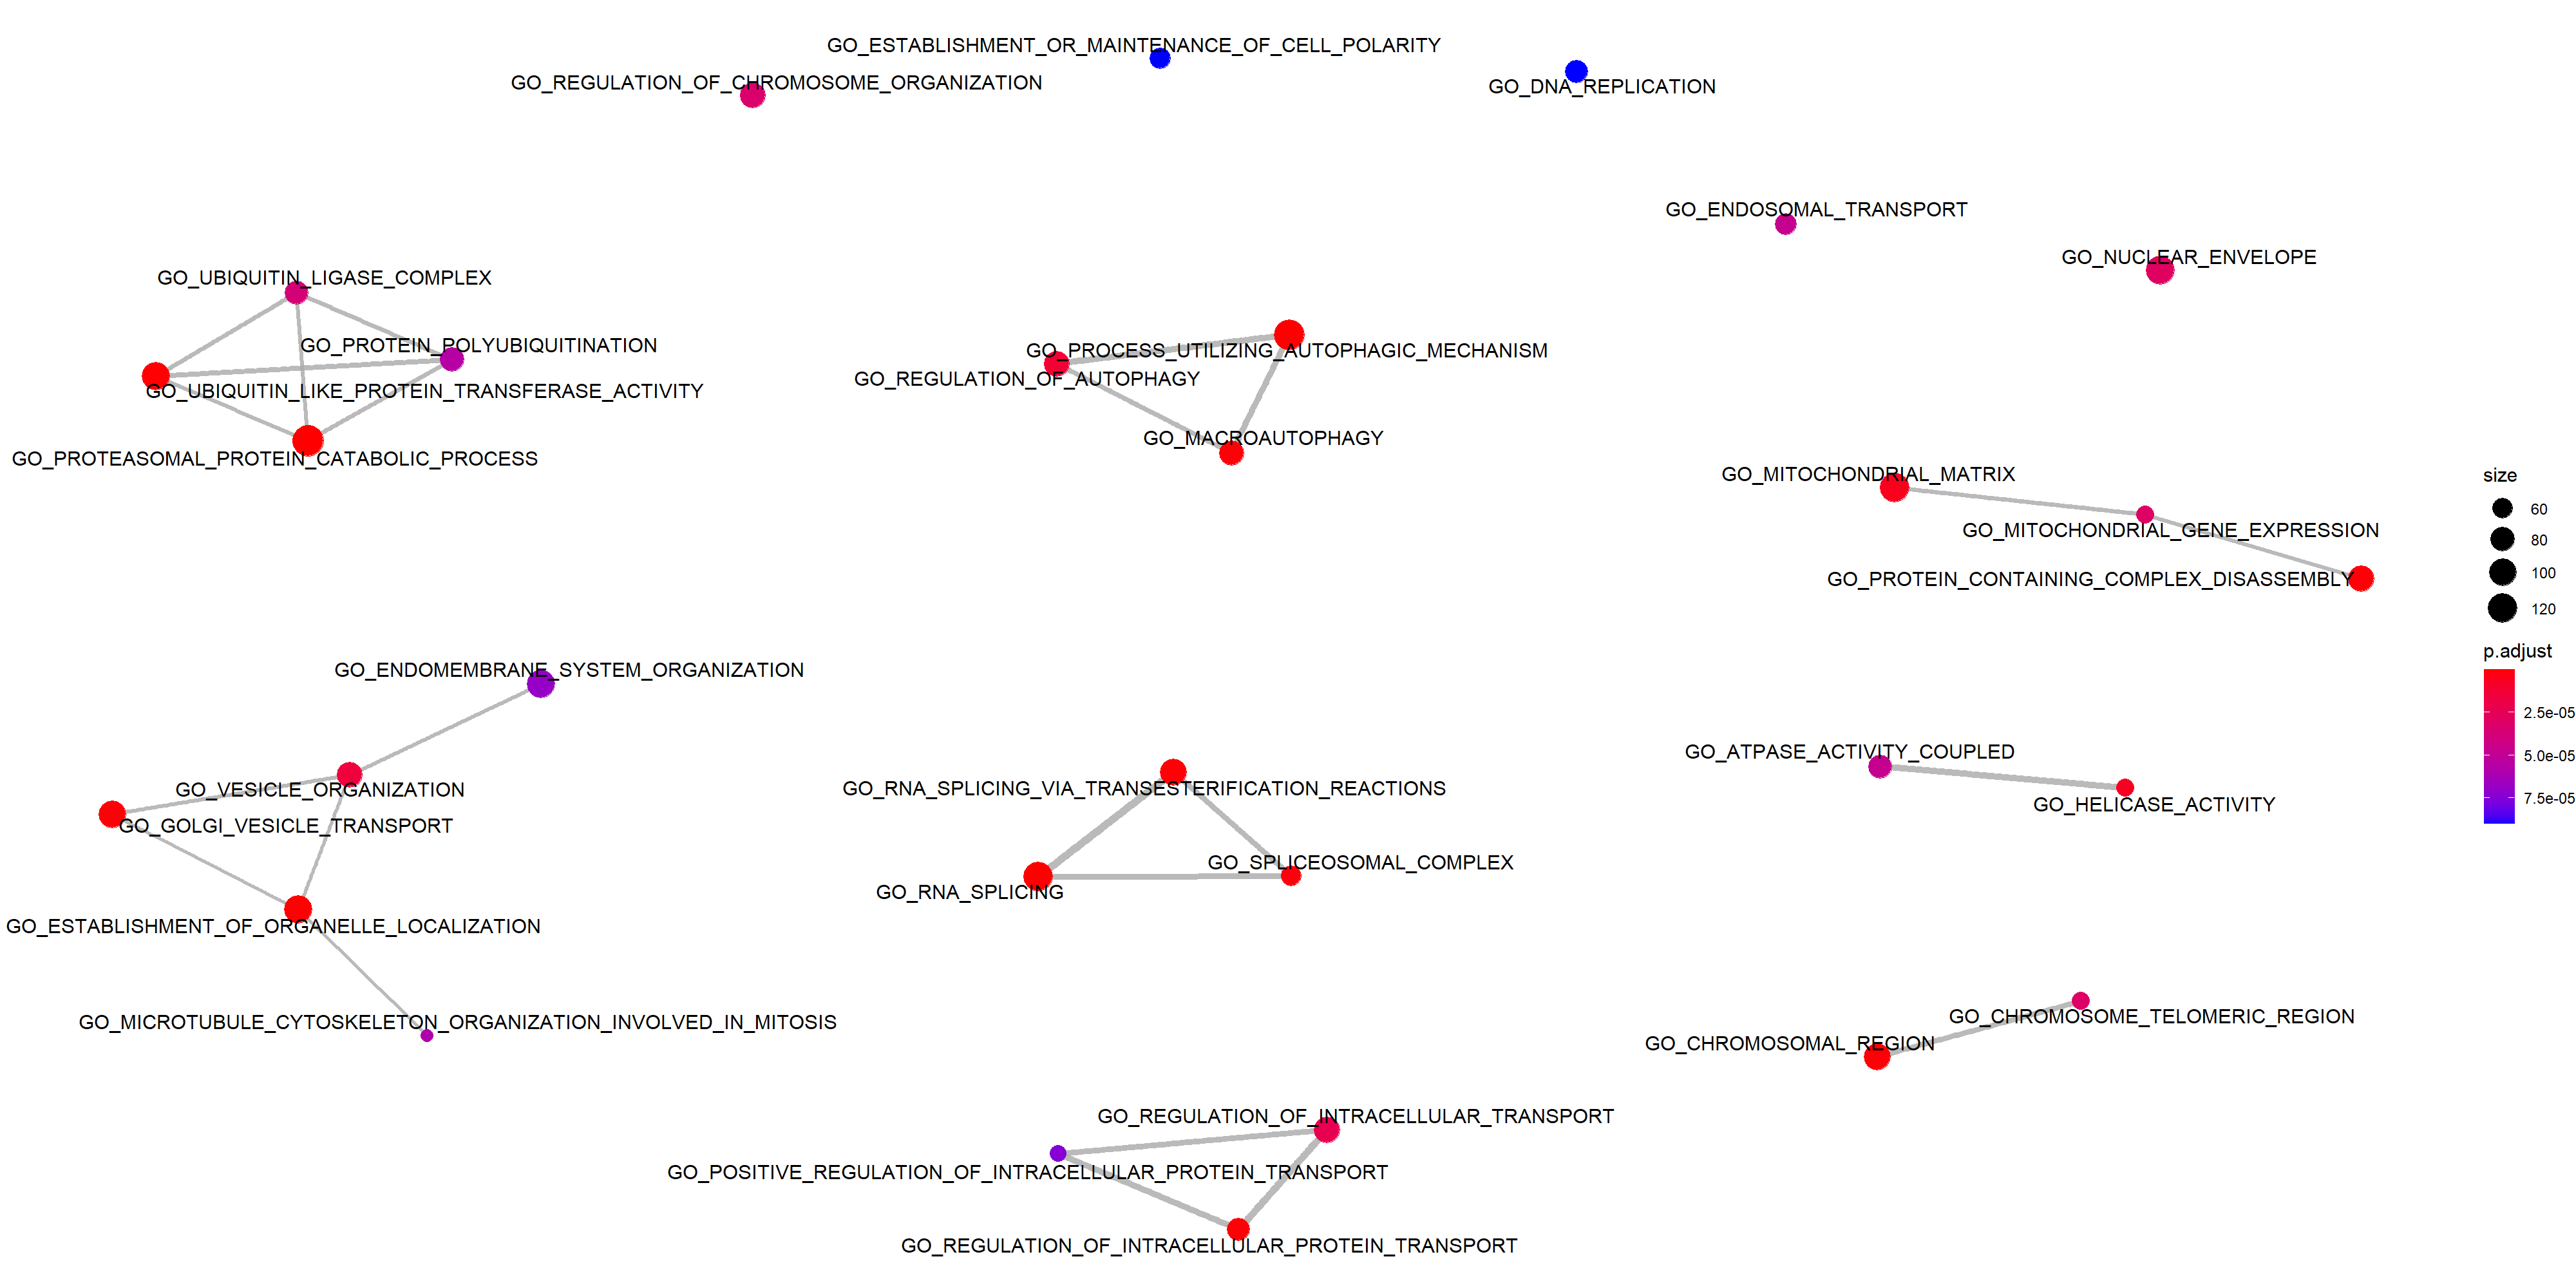
\includegraphics[width=10cm]{Figures/GSEA/CTLvs2bl_em_emapplot.png} }}%
    \\
    \subfloat[\centering Gene-concept network for ORA. ]{{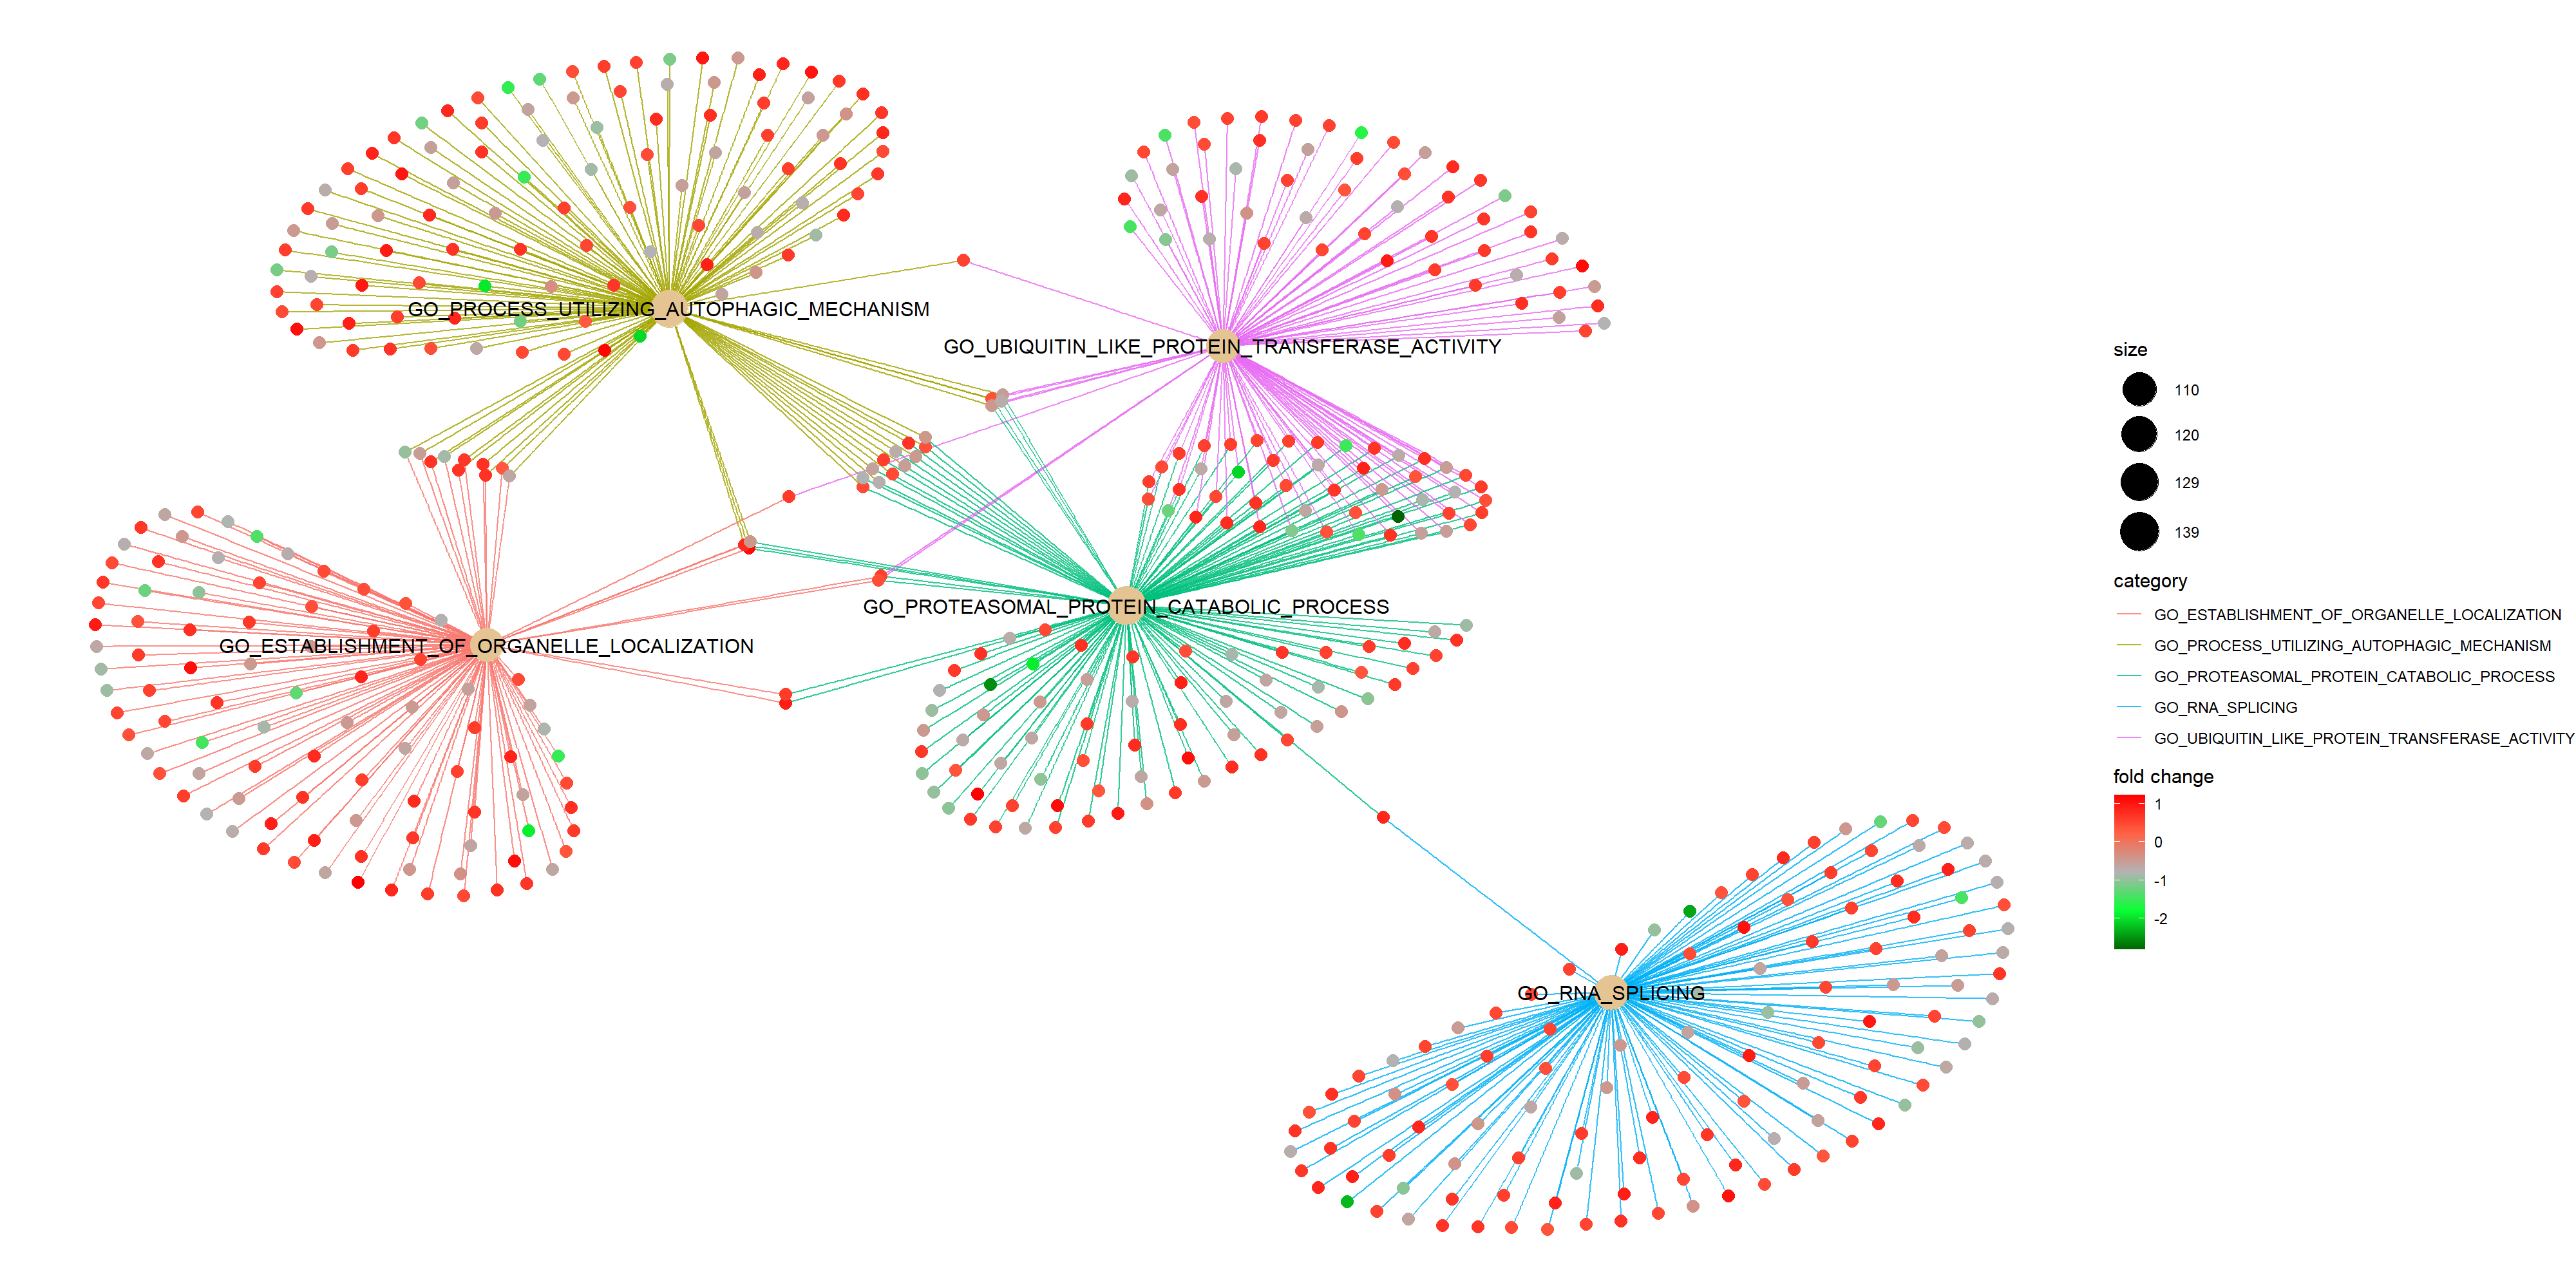
\includegraphics[width=10cm]{Figures/GSEA/CTLvs2bl_em_cnetplot.png} }}%
    \\
    \subfloat[\centering Heatmap for ORA. ]{{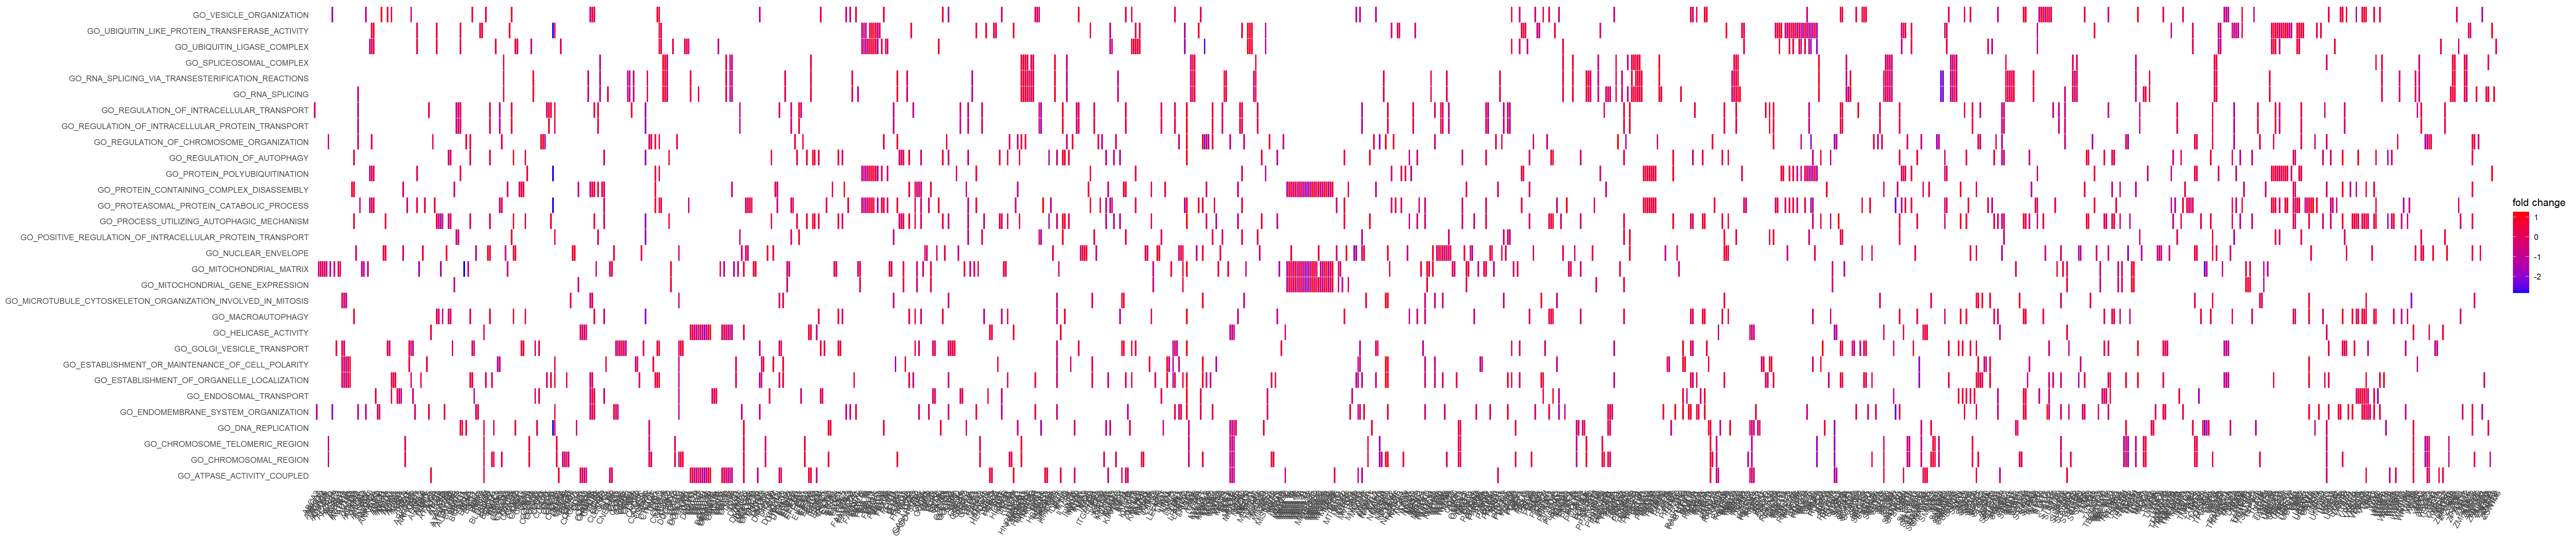
\includegraphics[width=10cm]{Figures/GSEA/CTLvs2bl_em_heatmap.png} }}%
\caption{Functional analysis visualizations of Blood-HD-m-S2.}
\end{figure}

% AD-Pa-f
\begin{figure}[!ht]%
    \centering
    \subfloat[\centering Enrichment map for ORA. ]{{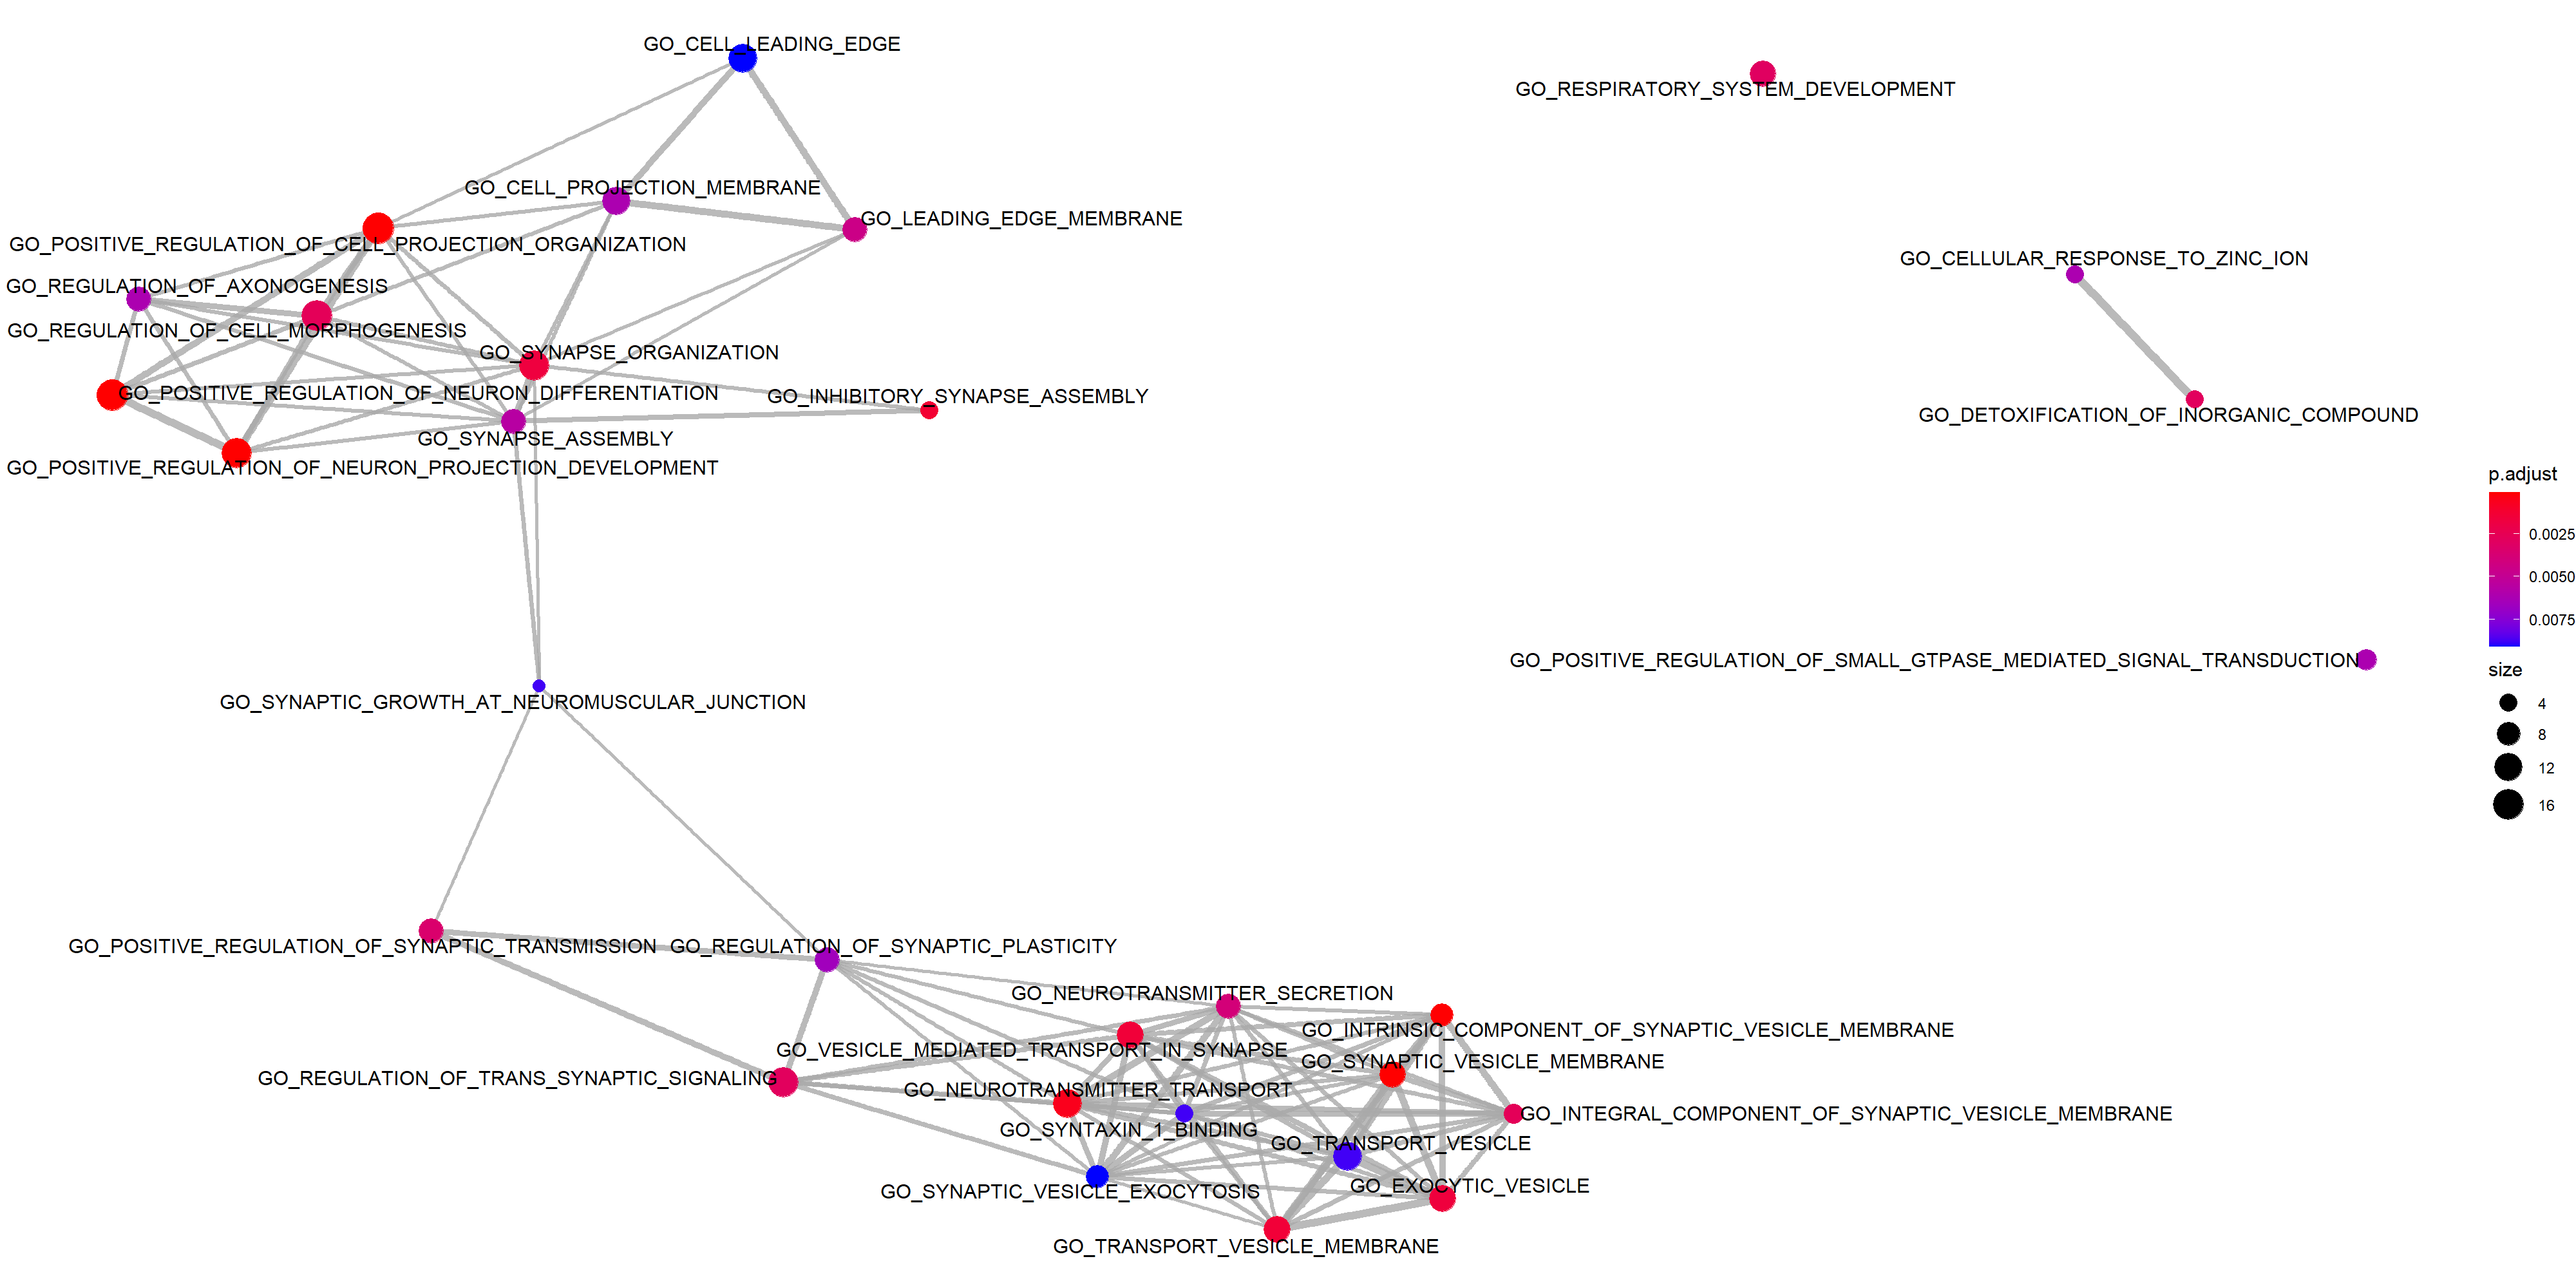
\includegraphics[width=10cm]{Figures/GSEA/CTLvsADpa_ef_emapplot.png} }}%
    \\
    \subfloat[\centering Gene-concept network for ORA. ]{{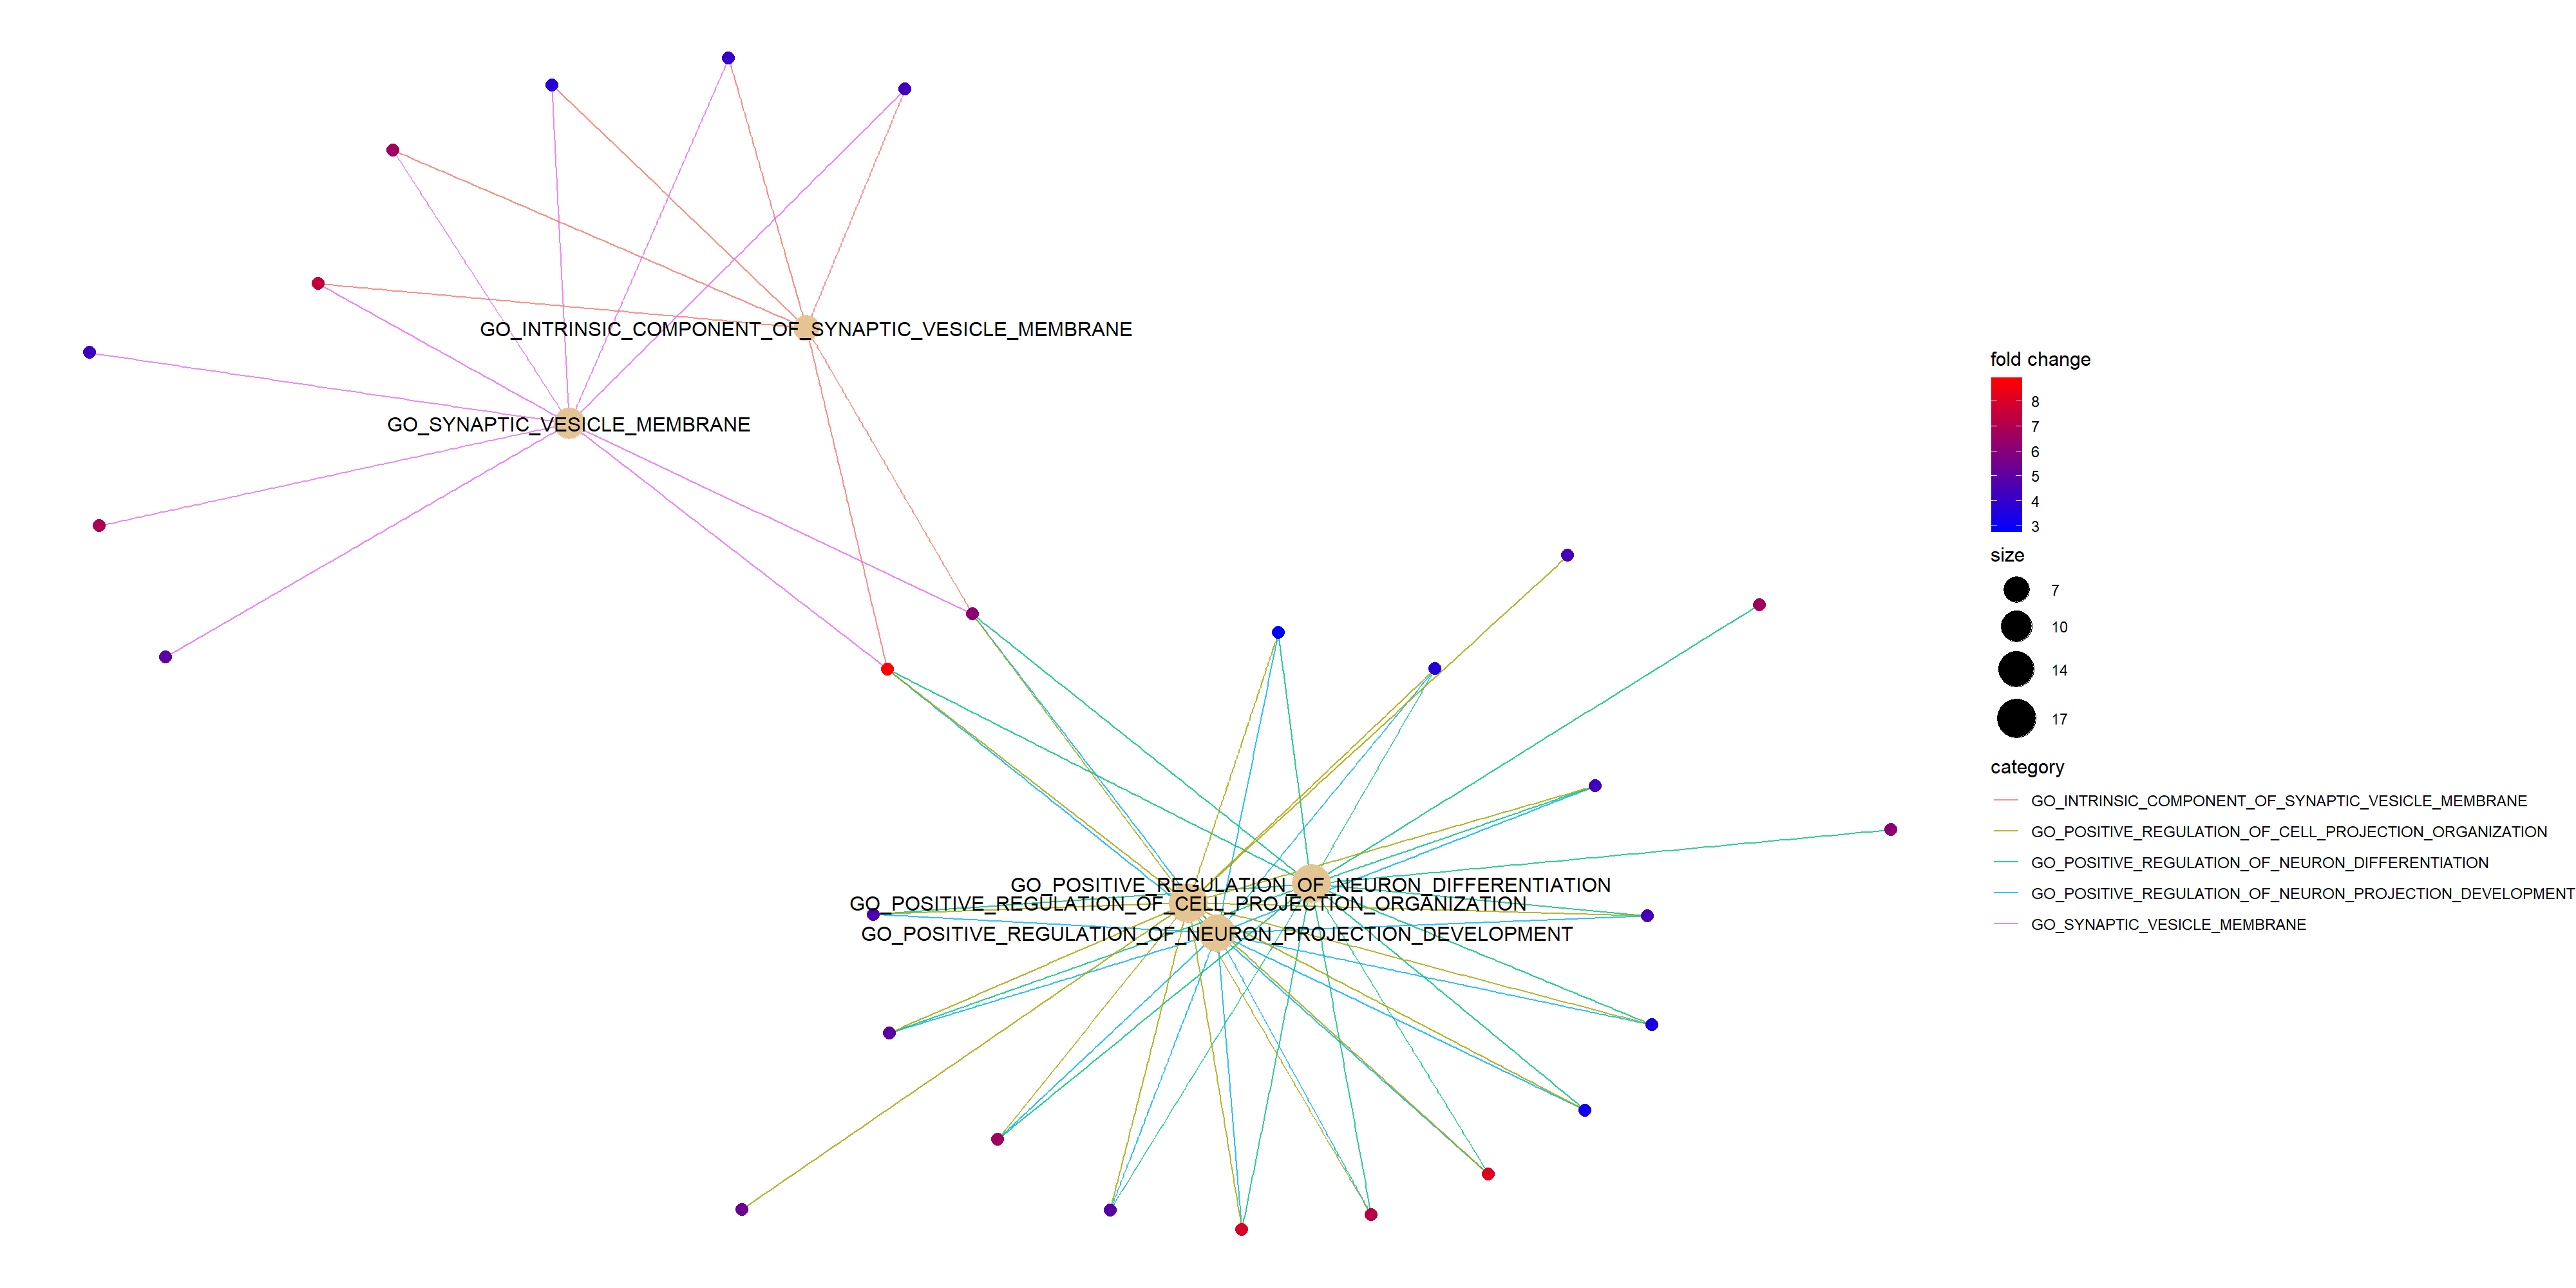
\includegraphics[width=10cm]{Figures/GSEA/CTLvsADpa_ef_cnetplot.png} }}%
    \\
    \subfloat[\centering Heatmap for ORA. ]{{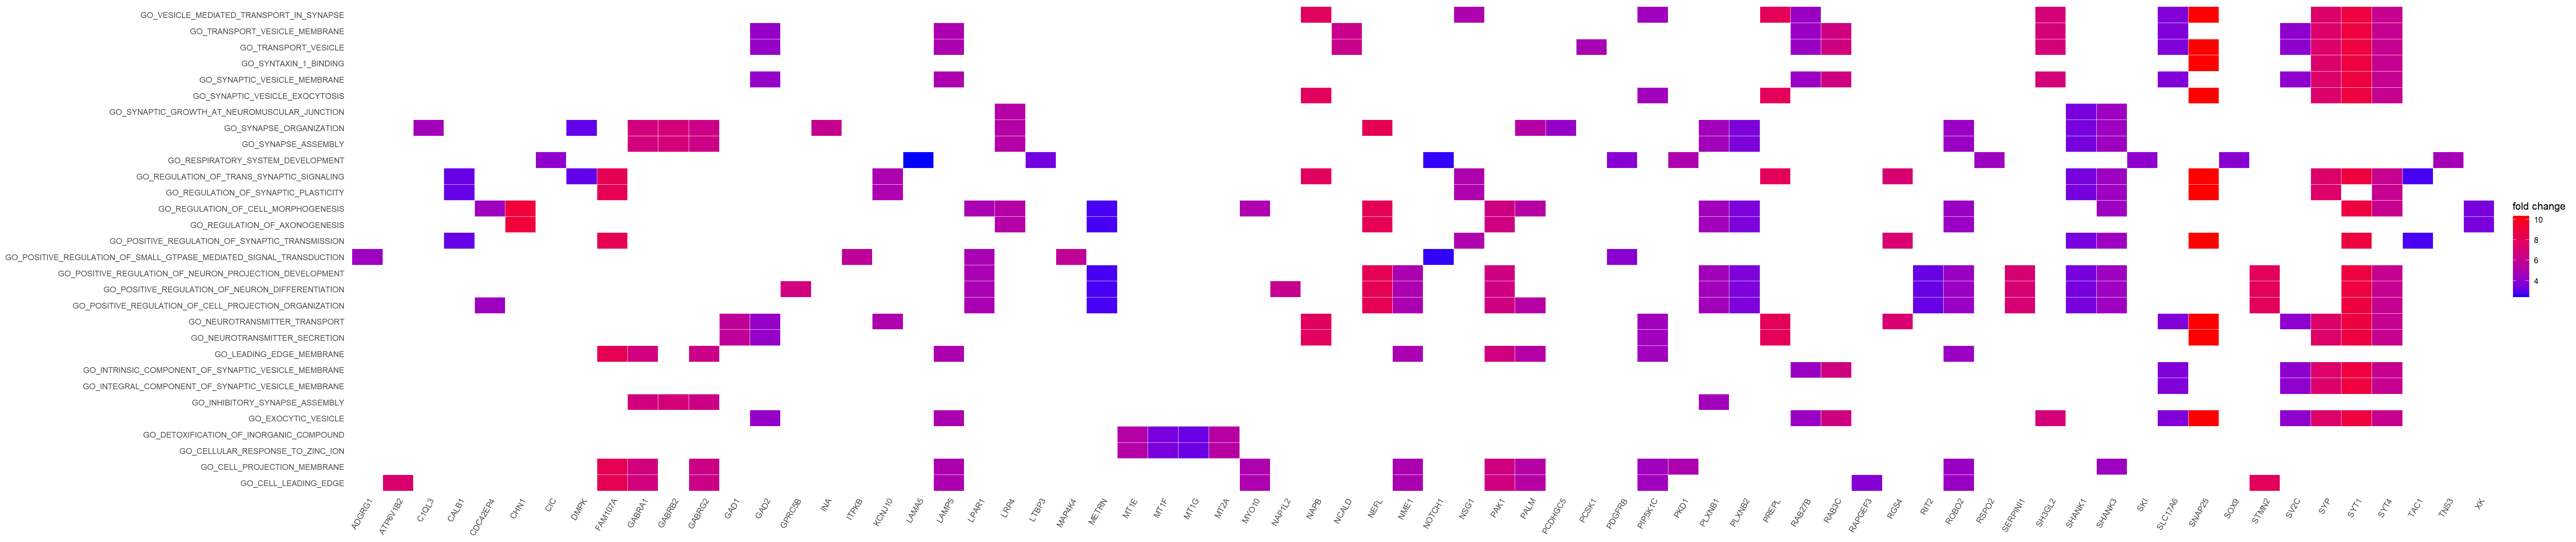
\includegraphics[width=10cm]{Figures/GSEA/CTLvsADpa_ef_heatmap.png} }}%
\caption{Functional analysis visualizations of Pa-AD-f.}
\end{figure}

% AD-Pa-m
\begin{figure}[!ht]%
    \centering
    \subfloat[\centering Enrichment map for ORA. ]{{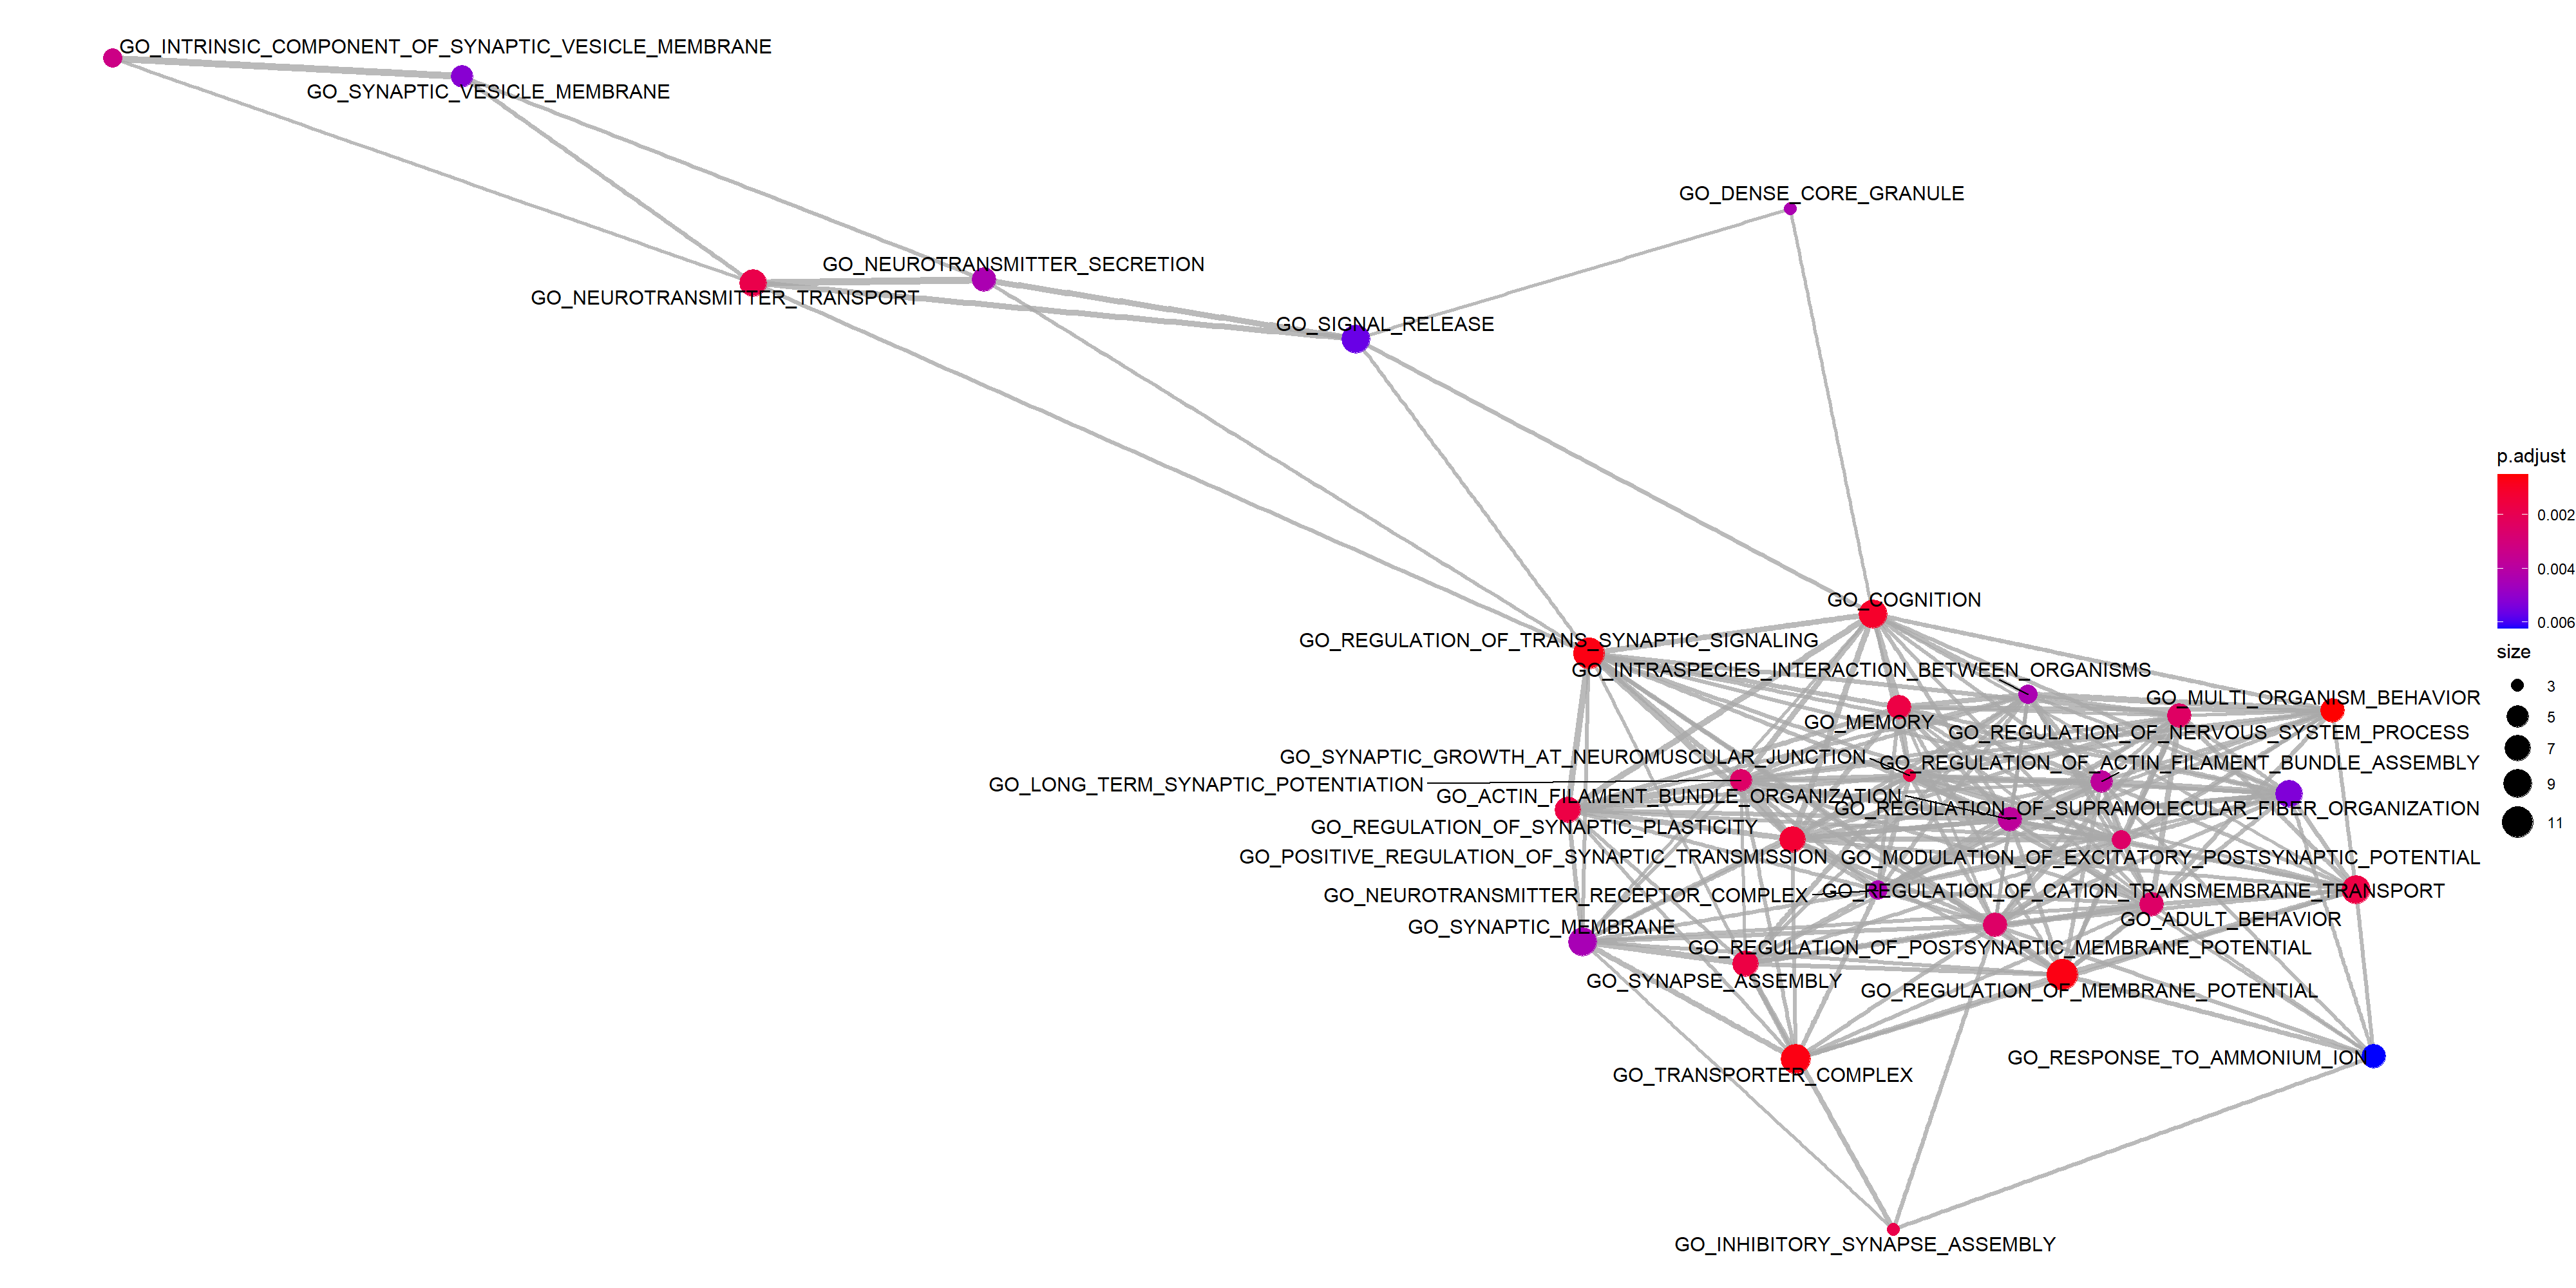
\includegraphics[width=10cm]{Figures/GSEA/CTLvsADpa_em_emapplot.png} }}%
    \\
    \subfloat[\centering Gene-concept network for ORA. ]{{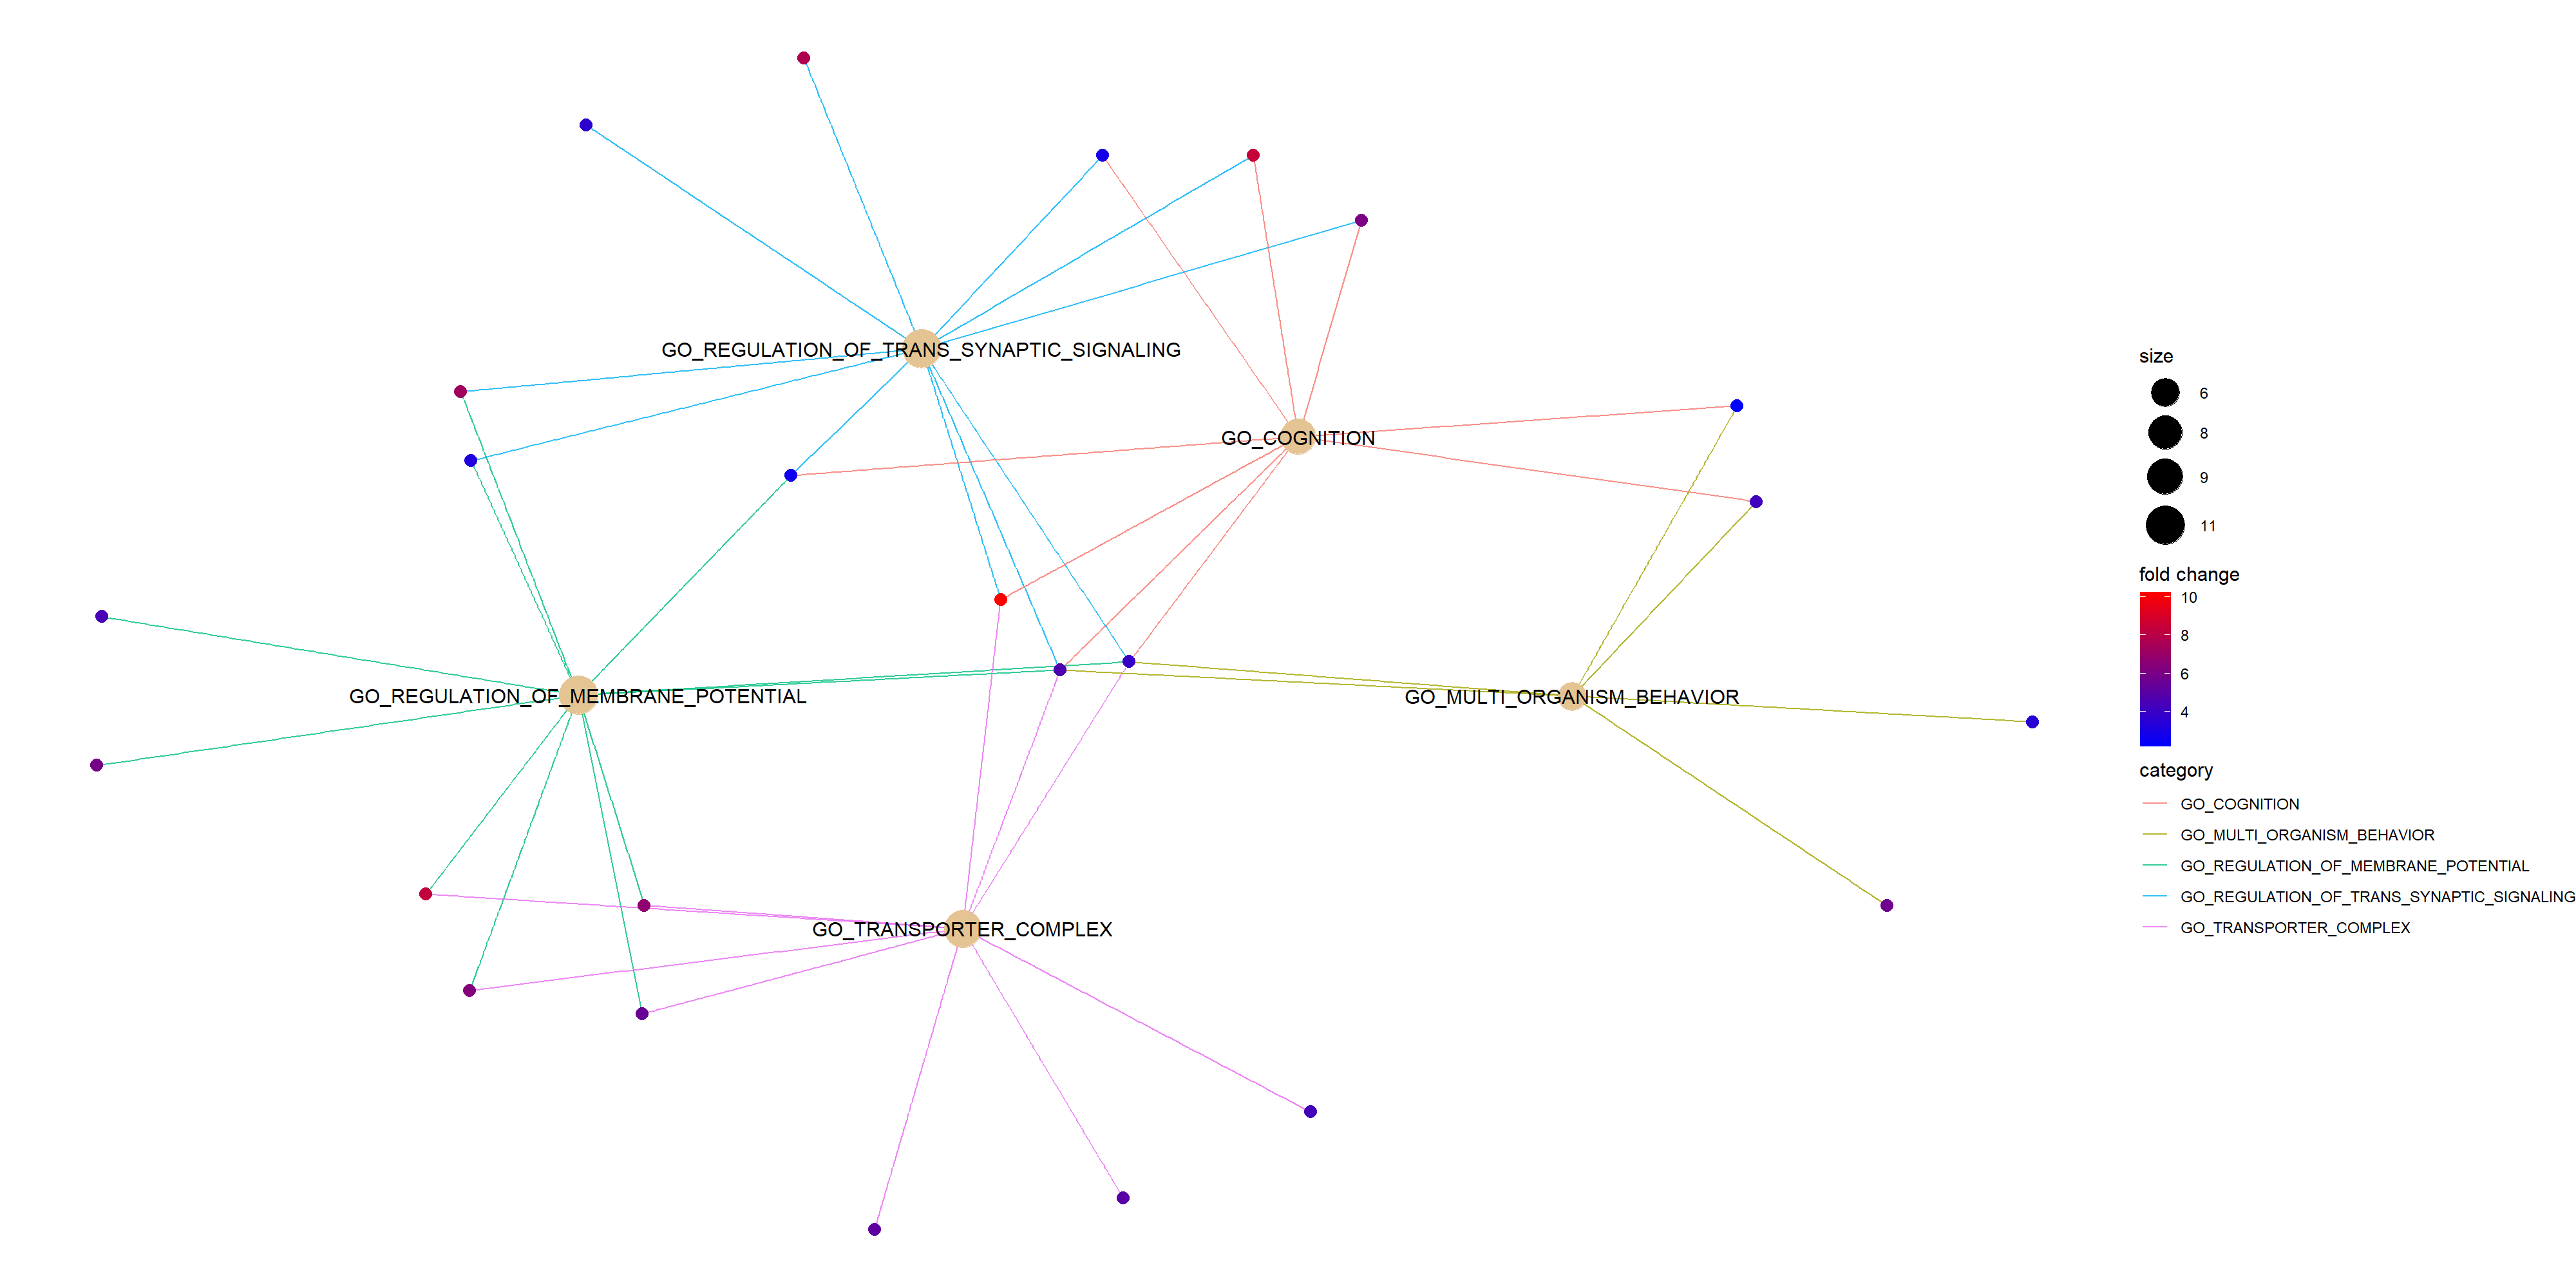
\includegraphics[width=10cm]{Figures/GSEA/CTLvsADpa_em_cnetplot.png} }}%
    \\
    \subfloat[\centering Heatmap for ORA. ]{{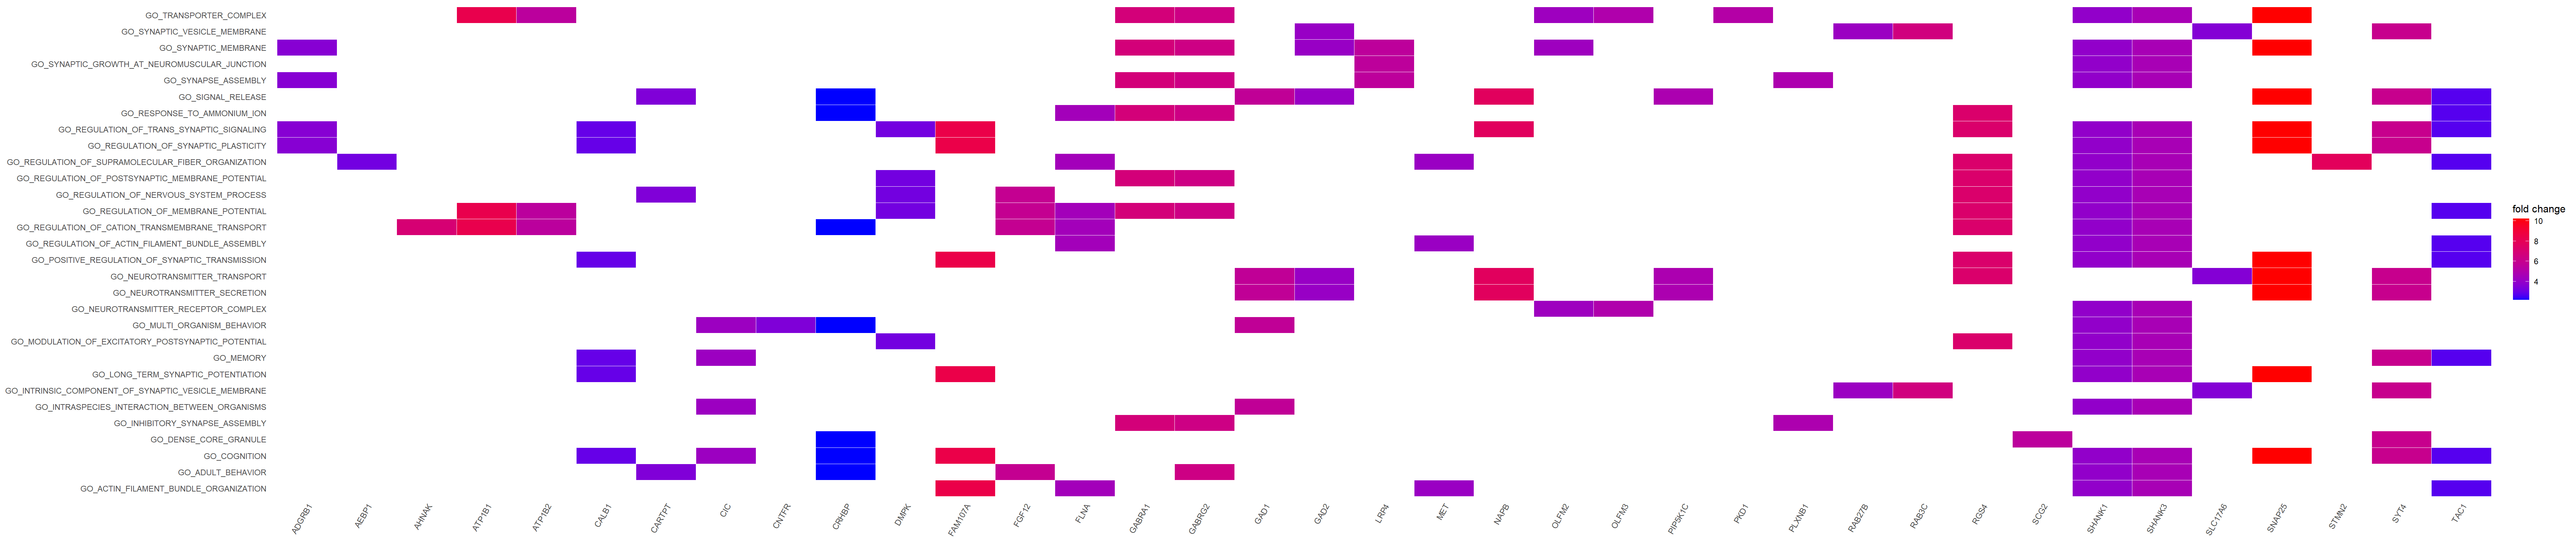
\includegraphics[width=10cm]{Figures/GSEA/CTLvsADpa_em_heatmap.png} }}%
\caption{Functional analysis visualizations of Pa-AD-m.}
\end{figure}

% AD-Temp-f
\begin{figure}[!ht]%
    \centering
    \subfloat[\centering Enrichment map for ORA. ]{{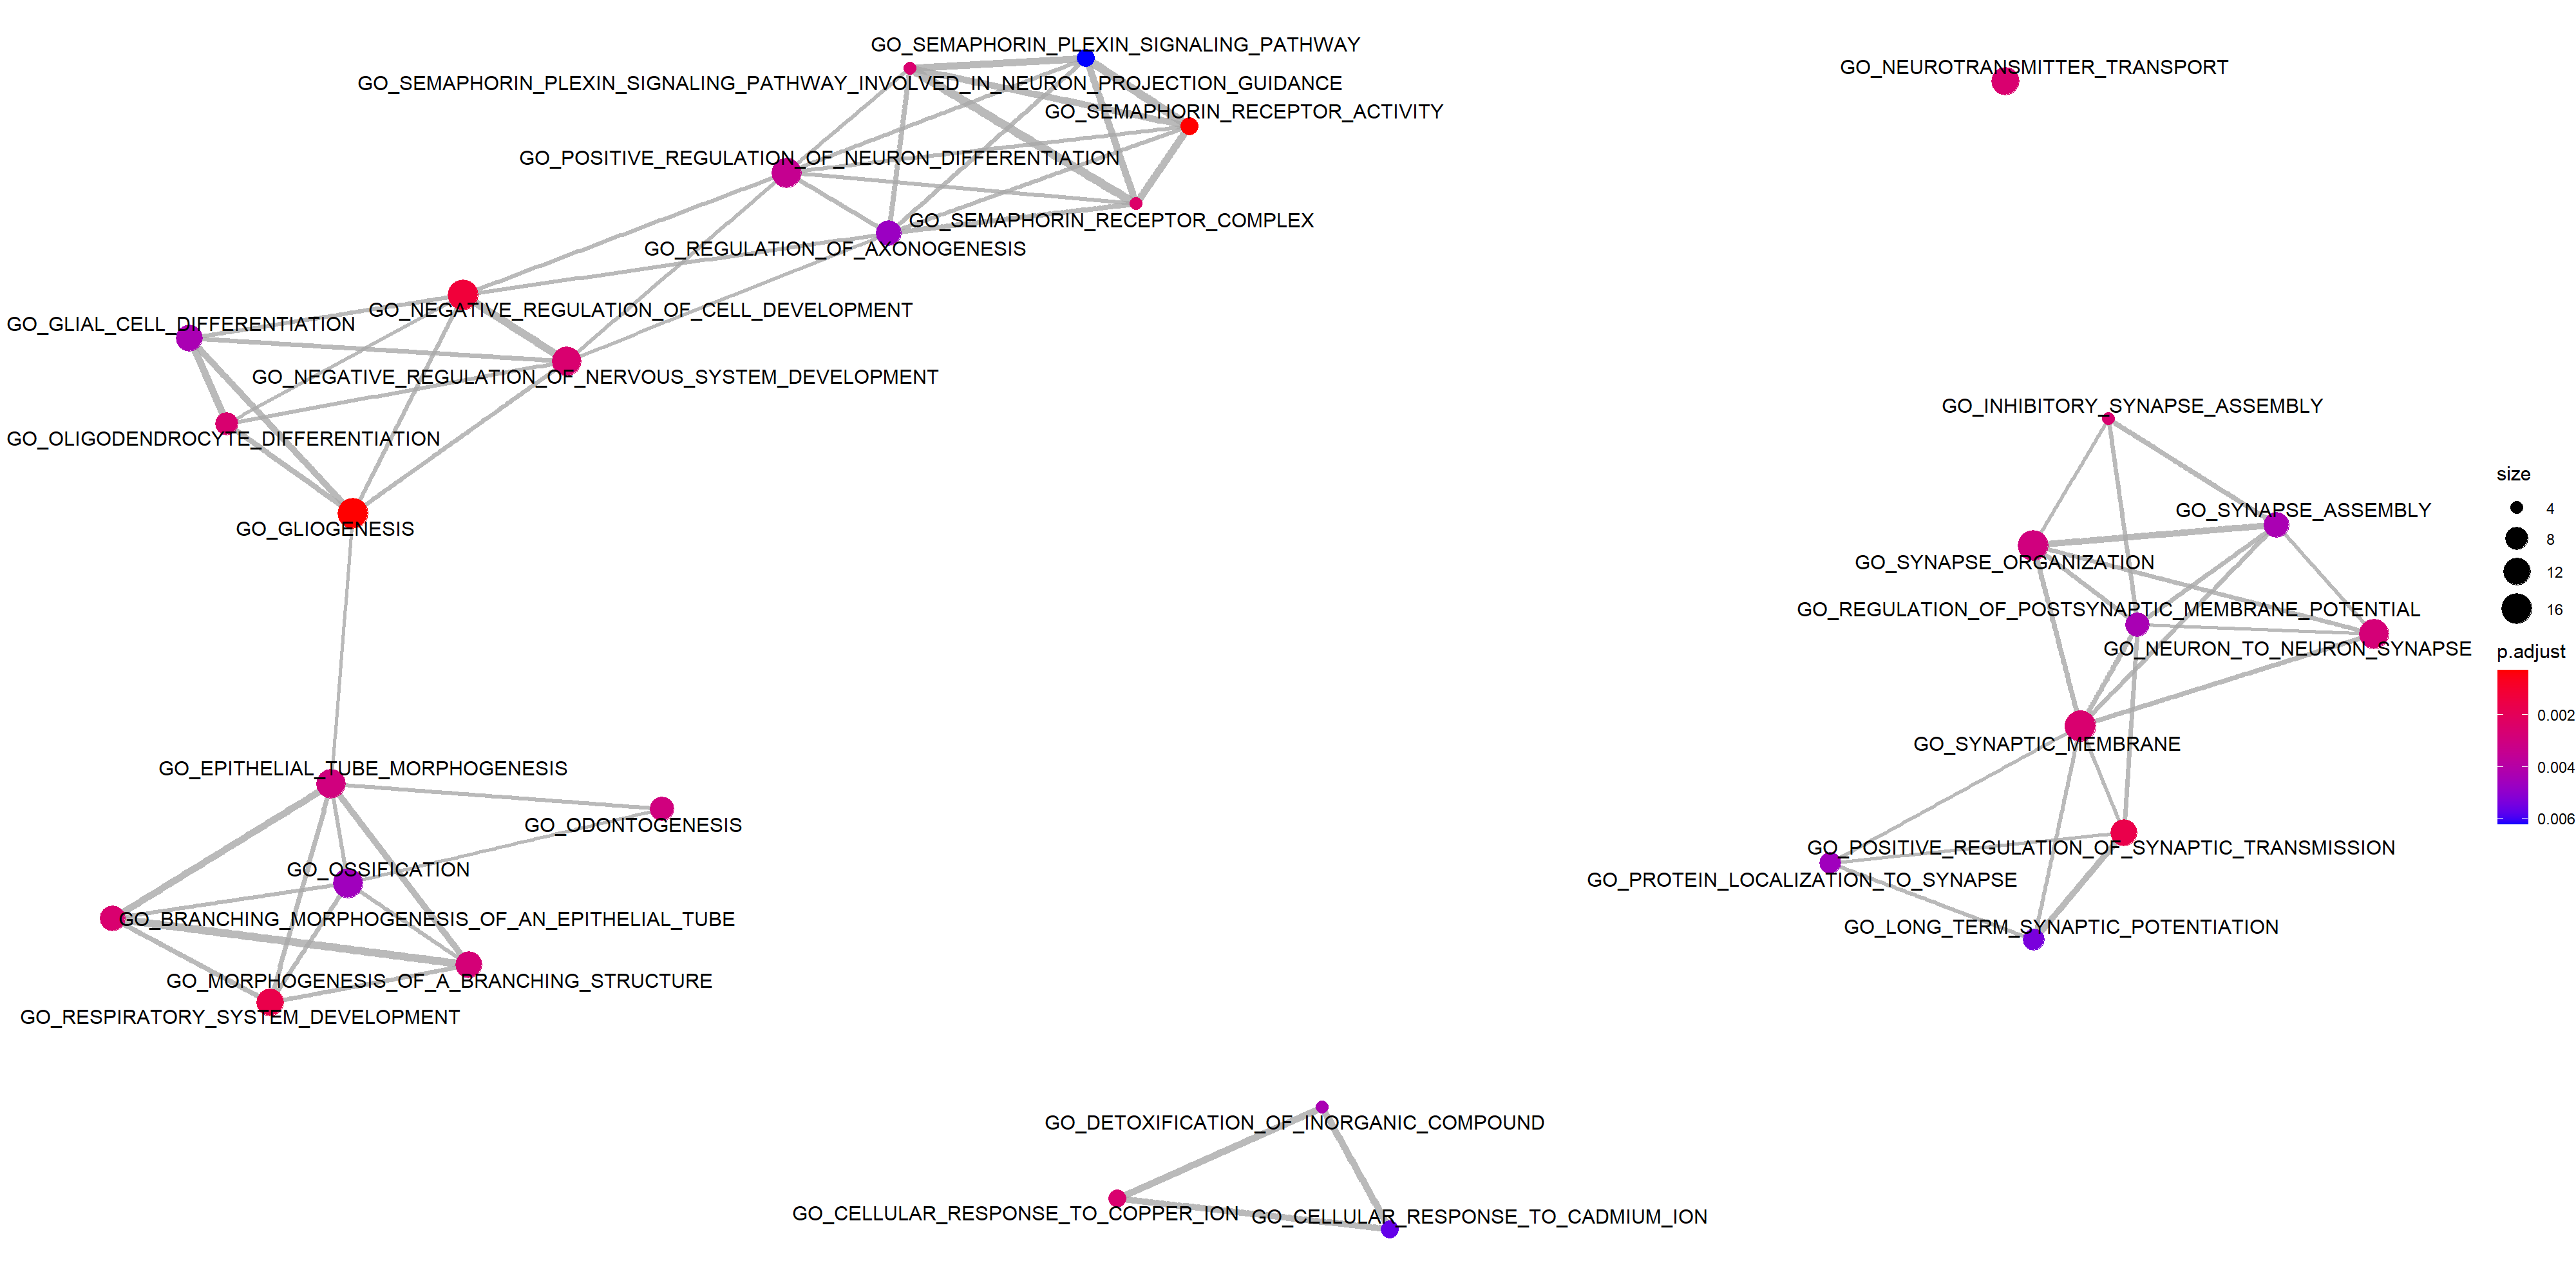
\includegraphics[width=10cm]{Figures/GSEA/CTLvsADte_ef_emapplot.png} }}%
    \\
    \subfloat[\centering Gene-concept network for ORA. ]{{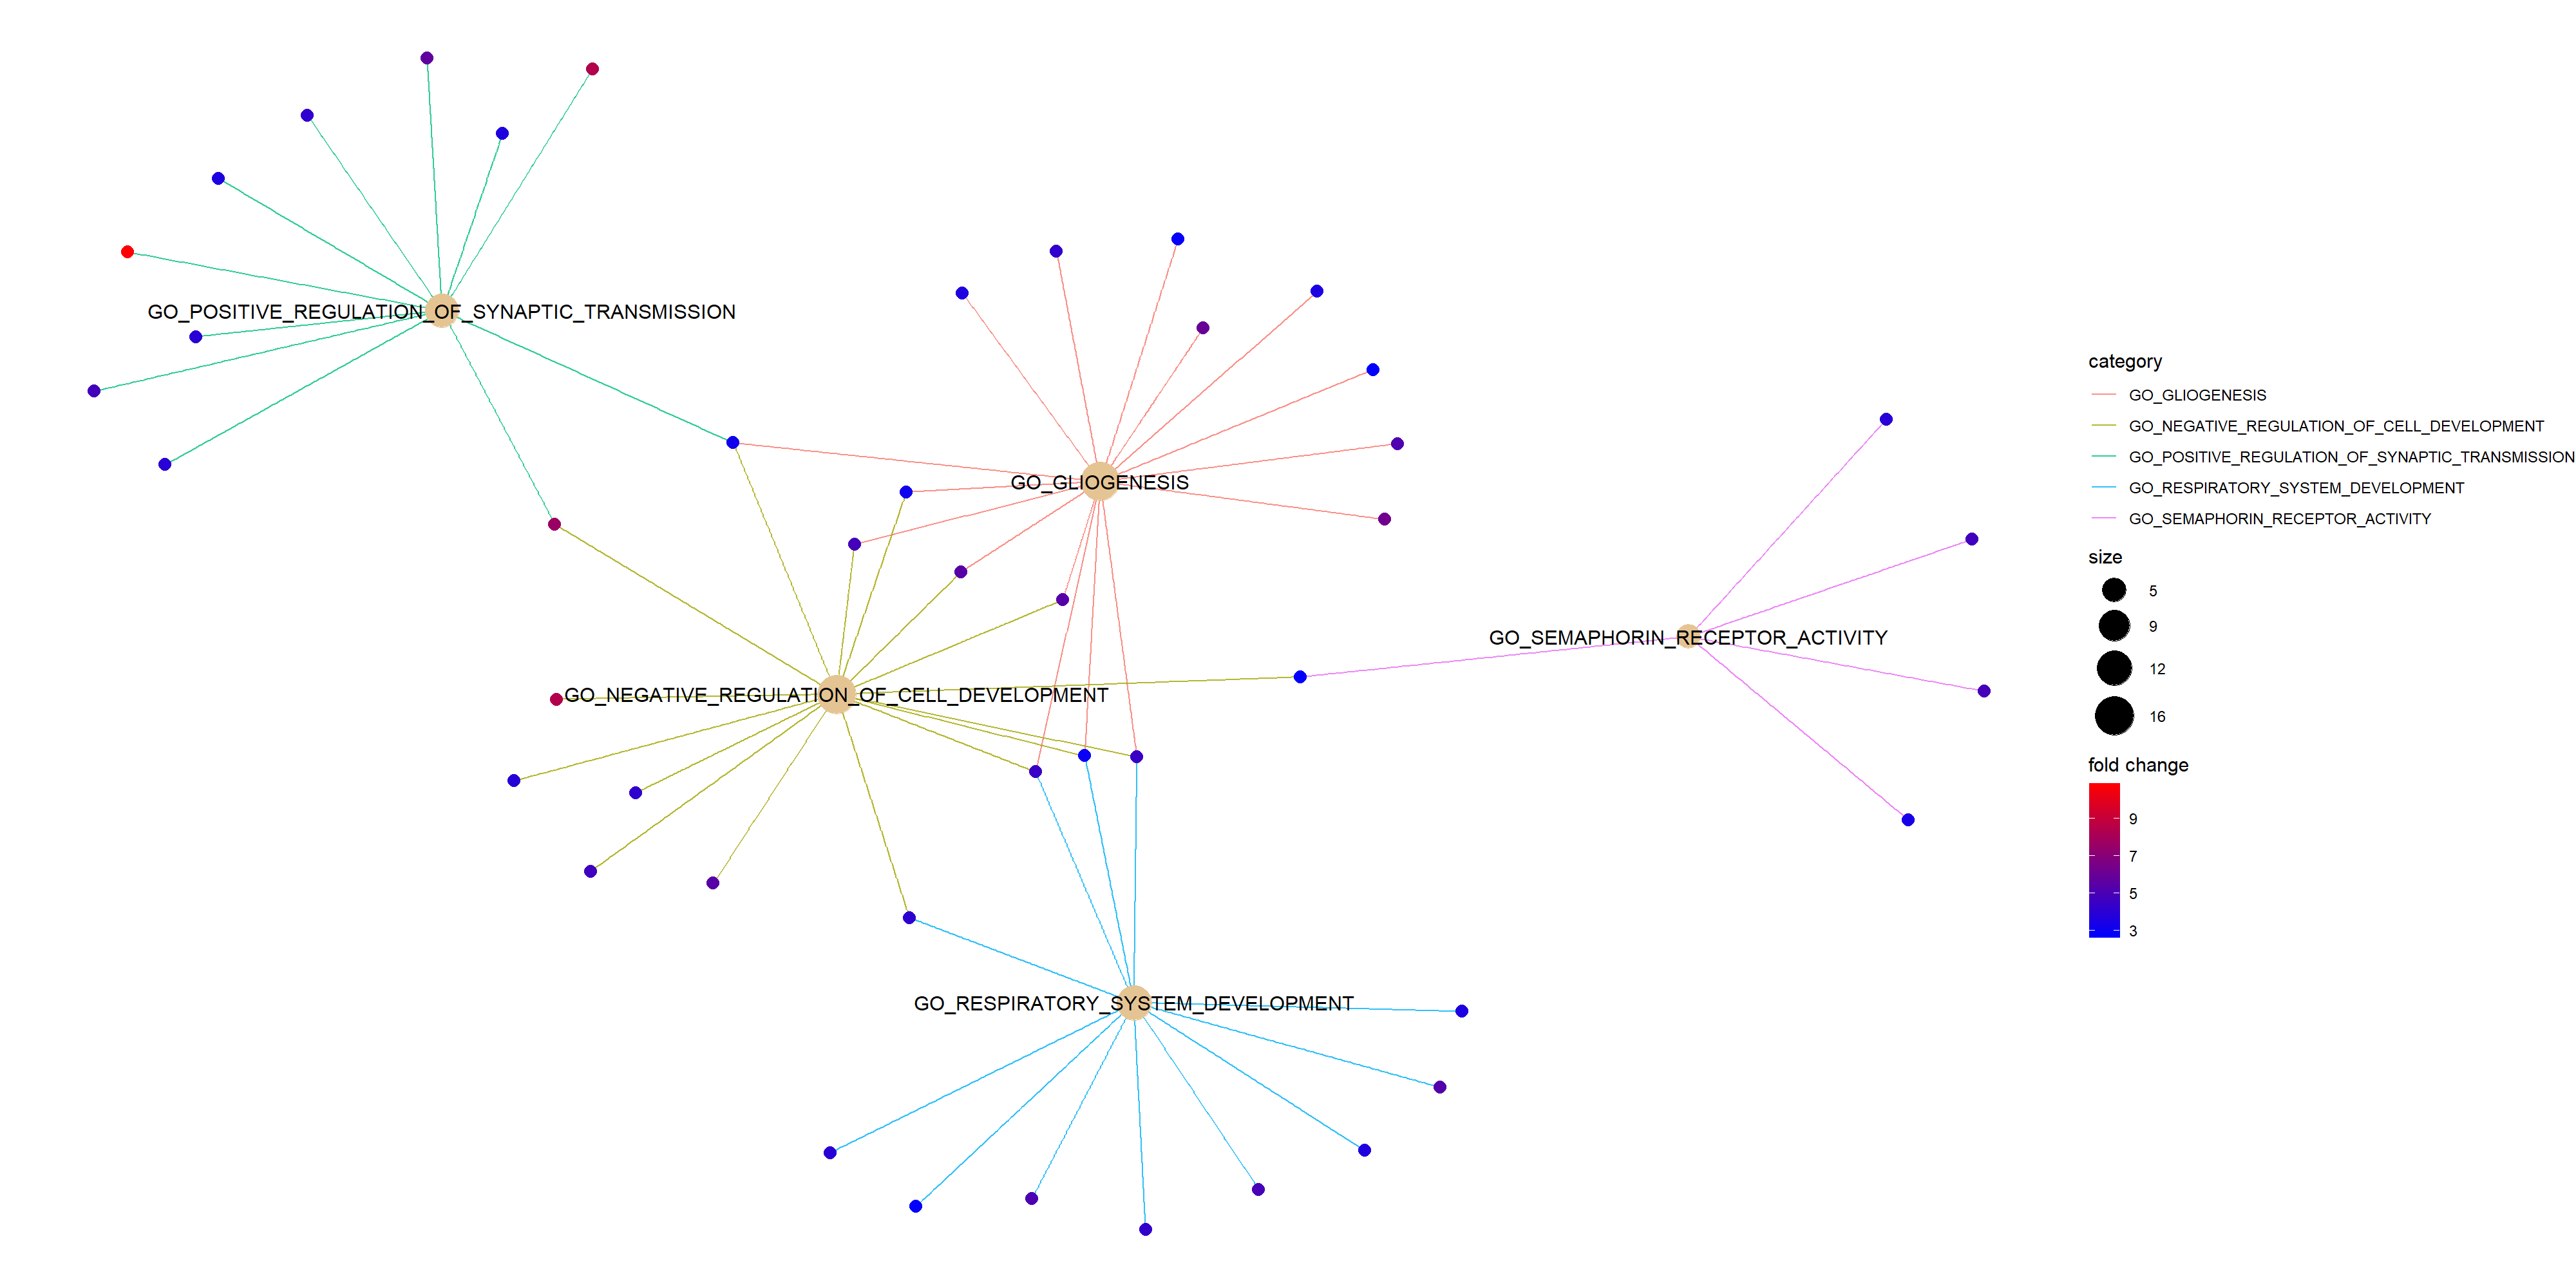
\includegraphics[width=10cm]{Figures/GSEA/CTLvsADte_ef_cnetplot.png} }}%
    \\
    \subfloat[\centering Heatmap for ORA. ]{{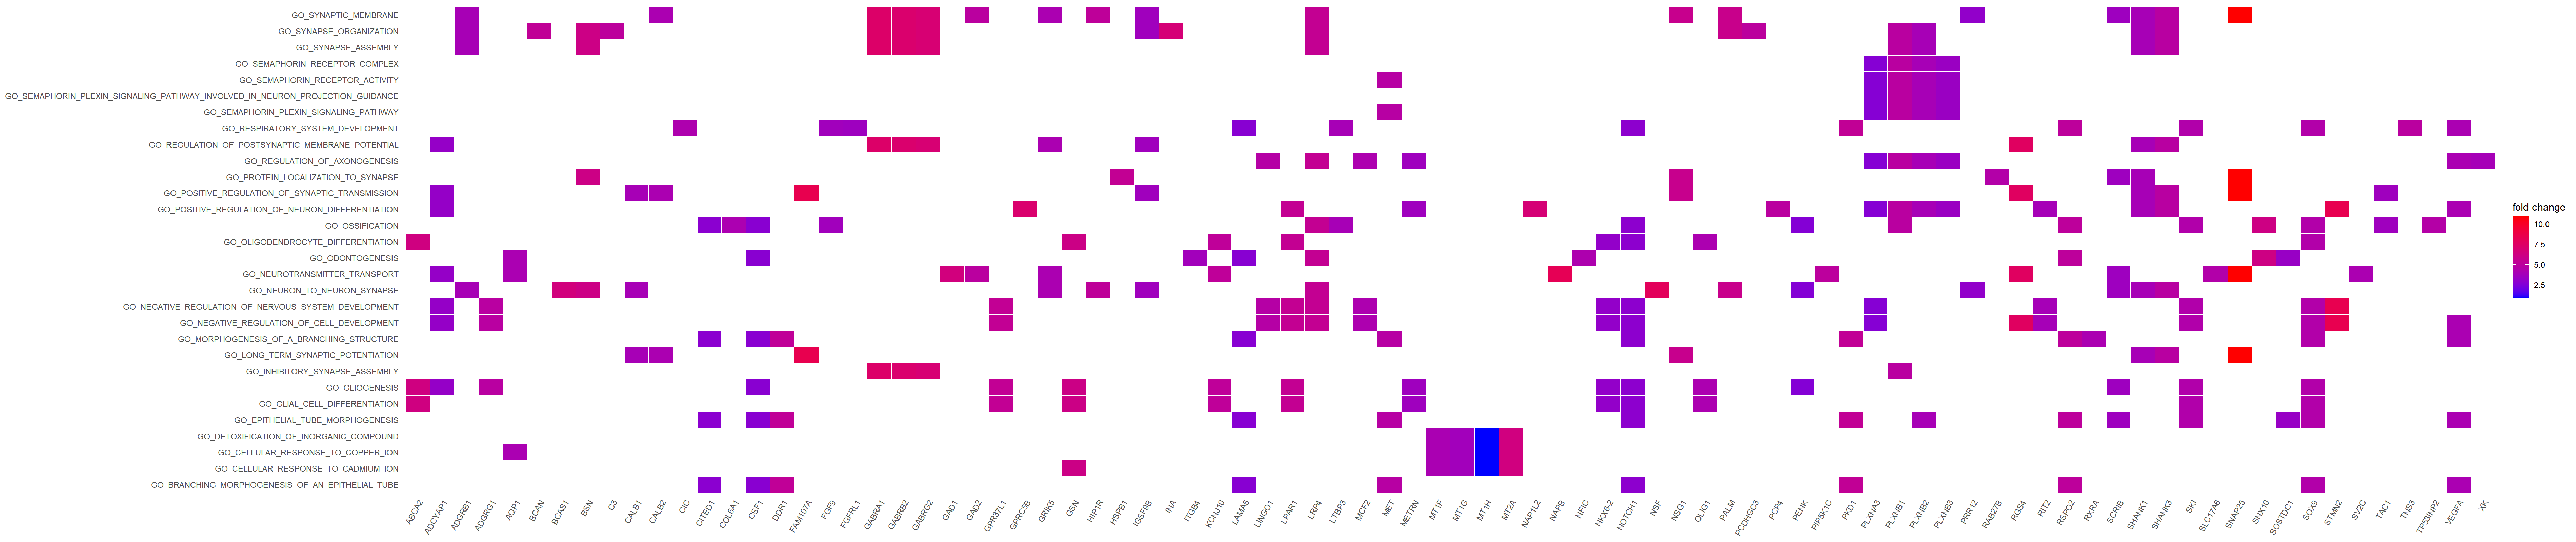
\includegraphics[width=10cm]{Figures/GSEA/CTLvsADte_ef_heatmap.png} }}%
\caption{Functional analysis visualizations of Temp-AD-f.}
\end{figure}

% AD-Temp-m
\begin{figure}[!ht]%
    \centering
    \subfloat[\centering Enrichment map for ORA. ]{{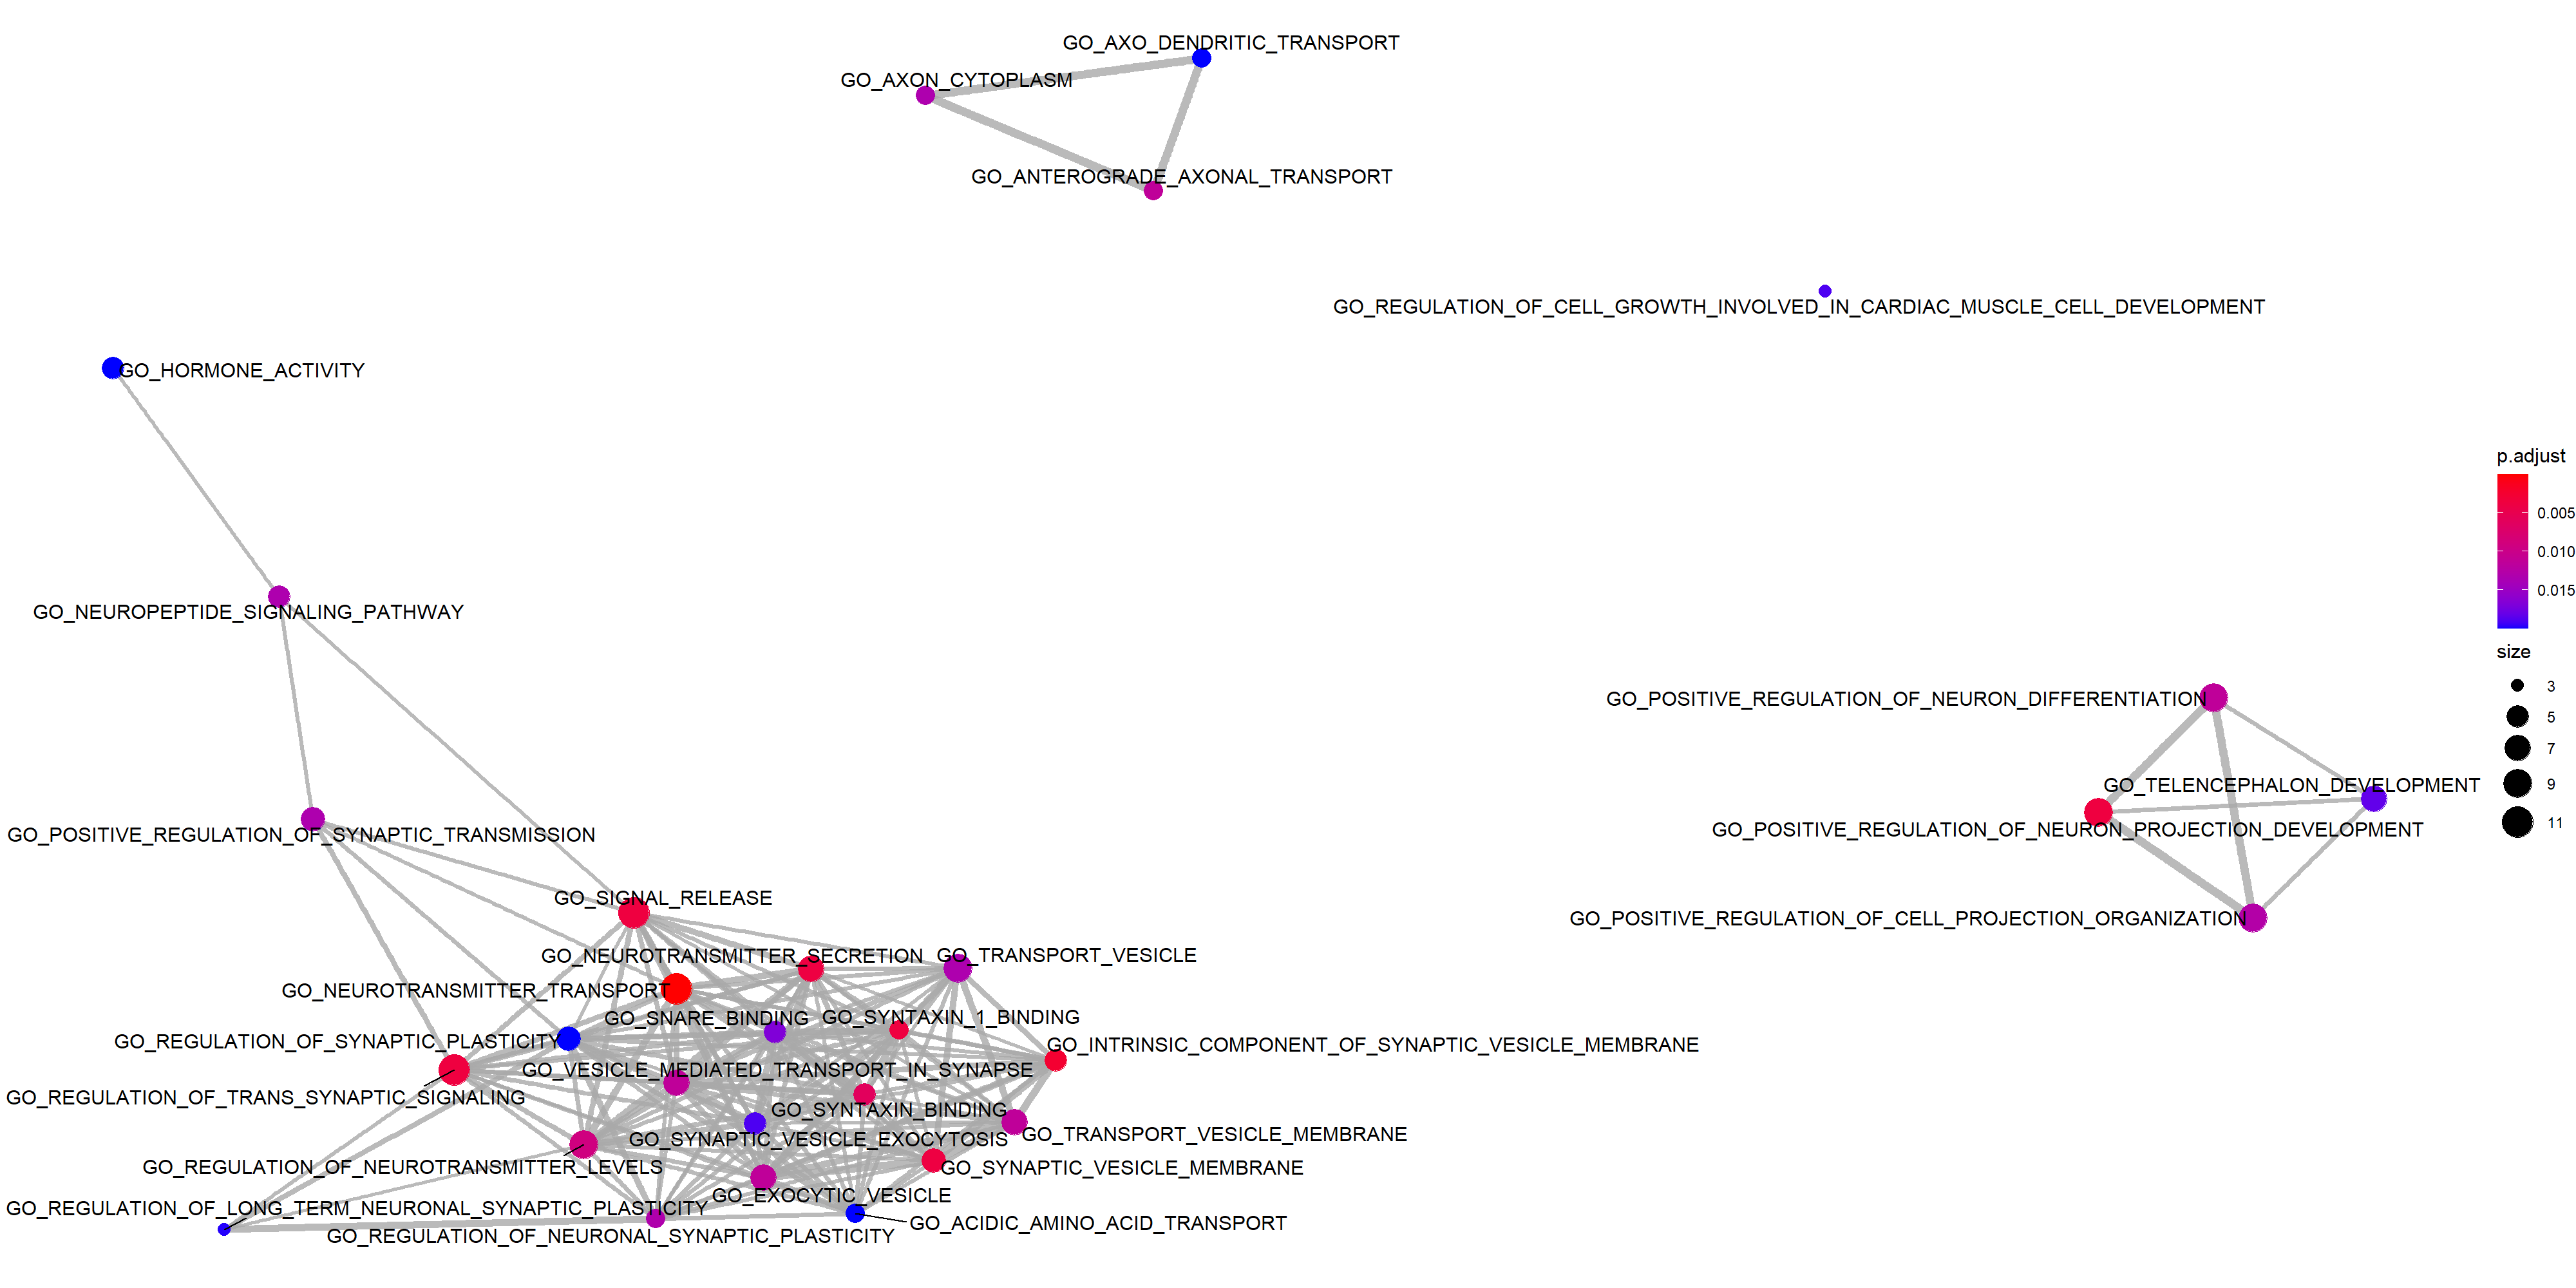
\includegraphics[width=10cm]{Figures/GSEA/CTLvsADte_em_emapplot.png} }}%
    \\
    \subfloat[\centering Gene-concept network for ORA. ]{{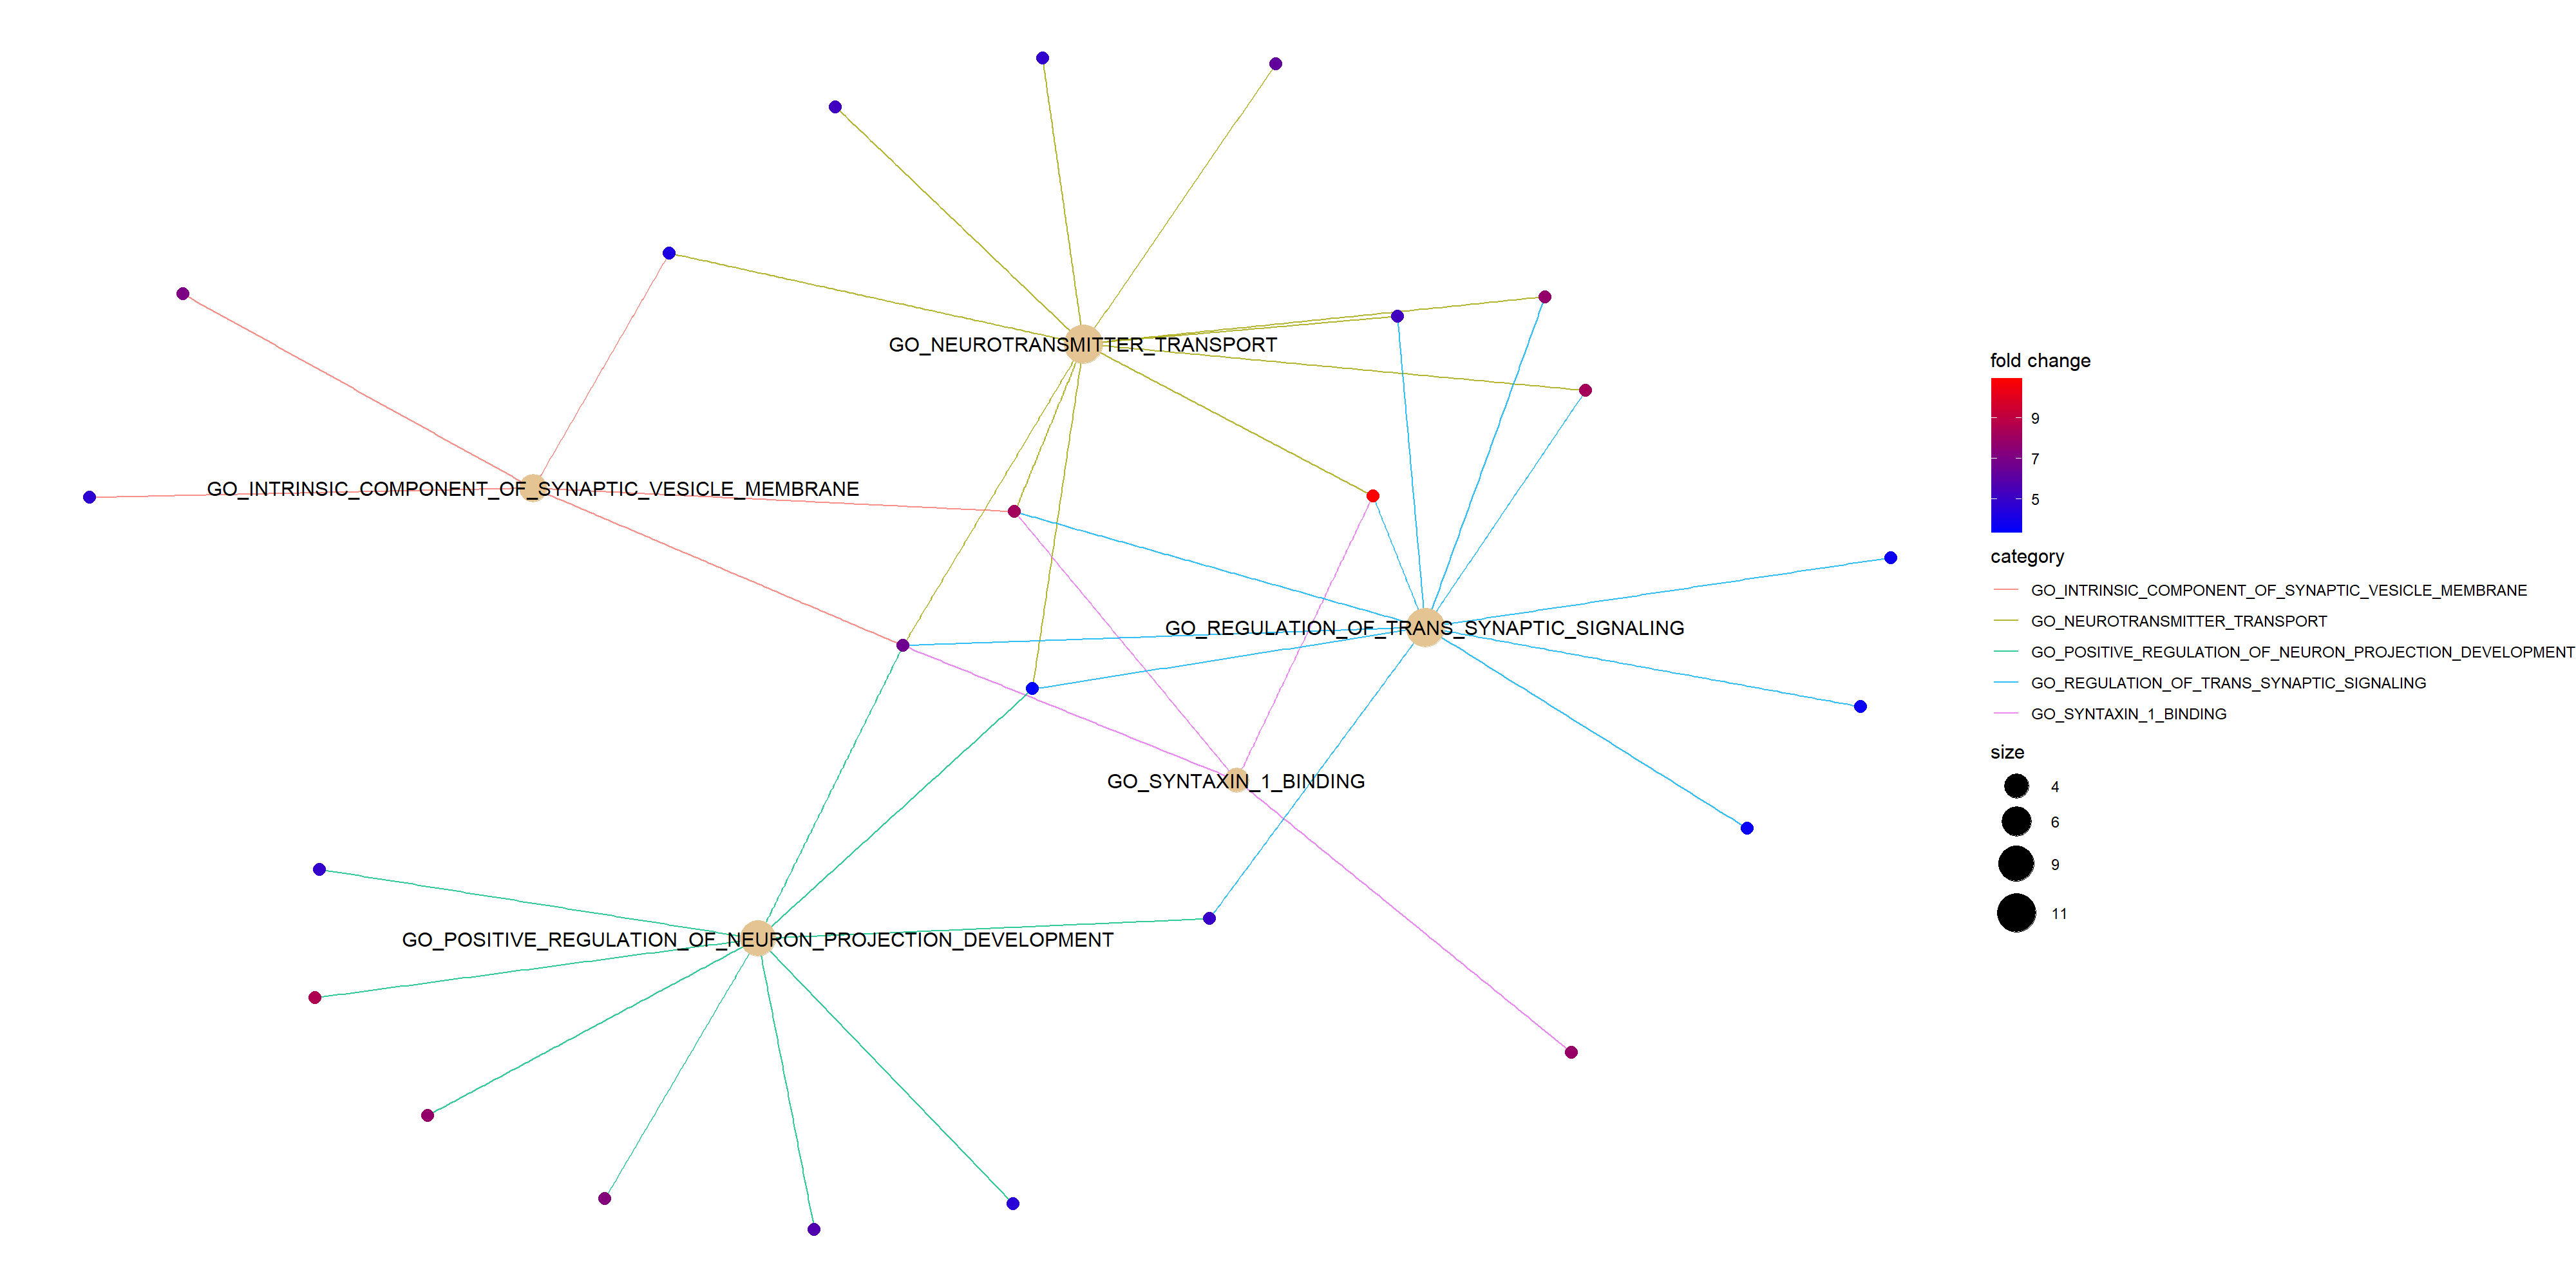
\includegraphics[width=10cm]{Figures/GSEA/CTLvsADte_em_cnetplot.png} }}%
    \\
    \subfloat[\centering Heatmap for ORA. ]{{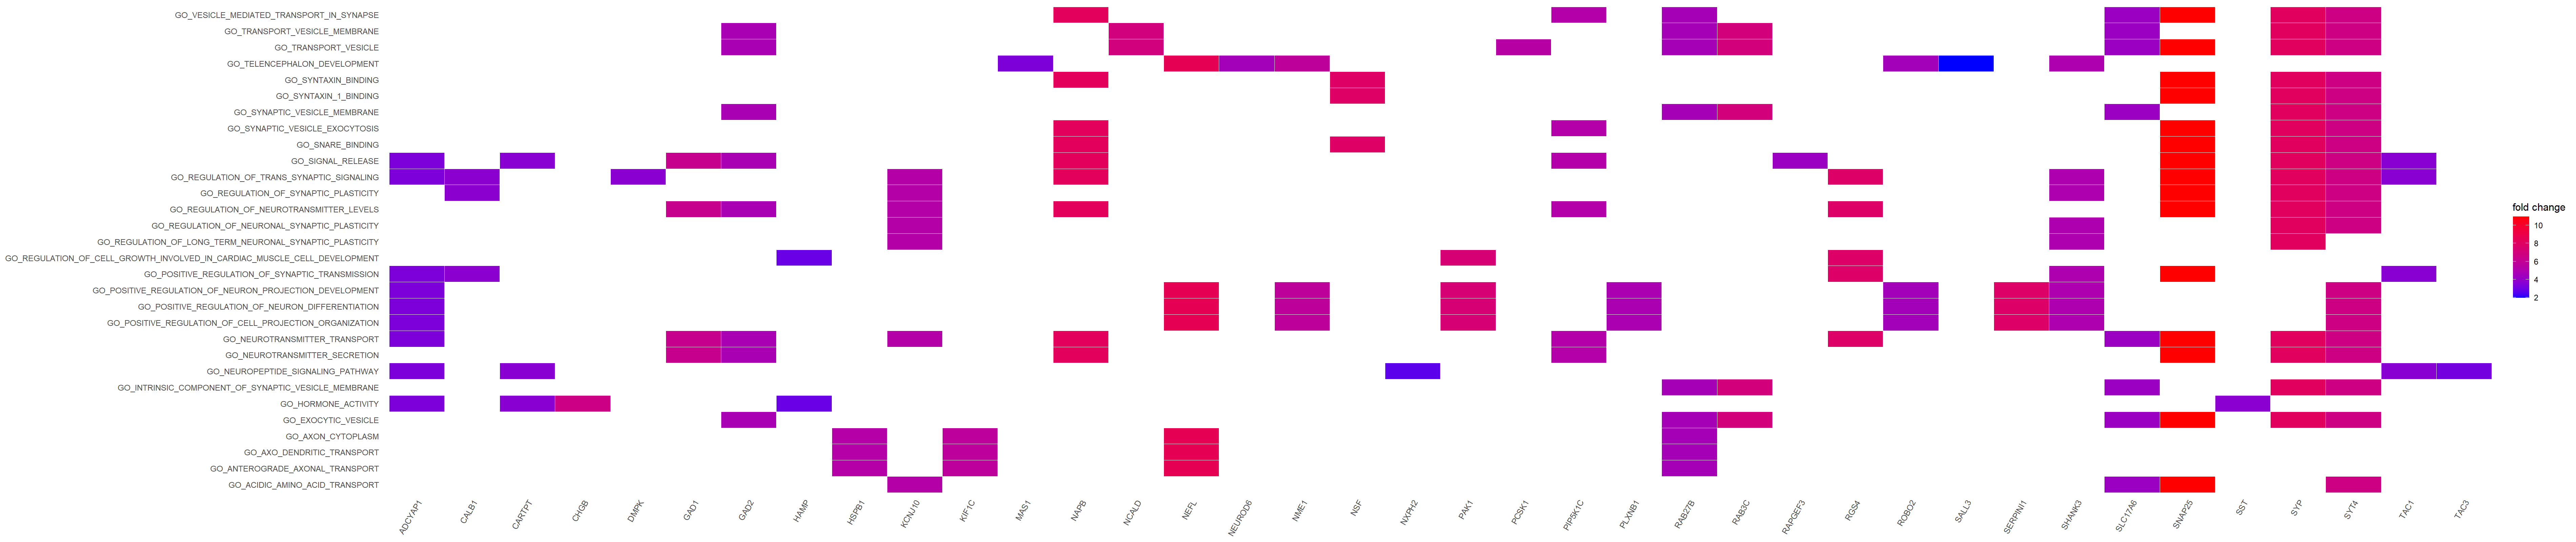
\includegraphics[width=10cm]{Figures/GSEA/CTLvsADte_em_heatmap.png} }}%
\caption{Functional analysis visualizations of Temp-AD-m.}
\end{figure}

% AD-Hip-f
\begin{figure}[!ht]%
    \centering
    \subfloat[\centering Enrichment map for ORA. ]{{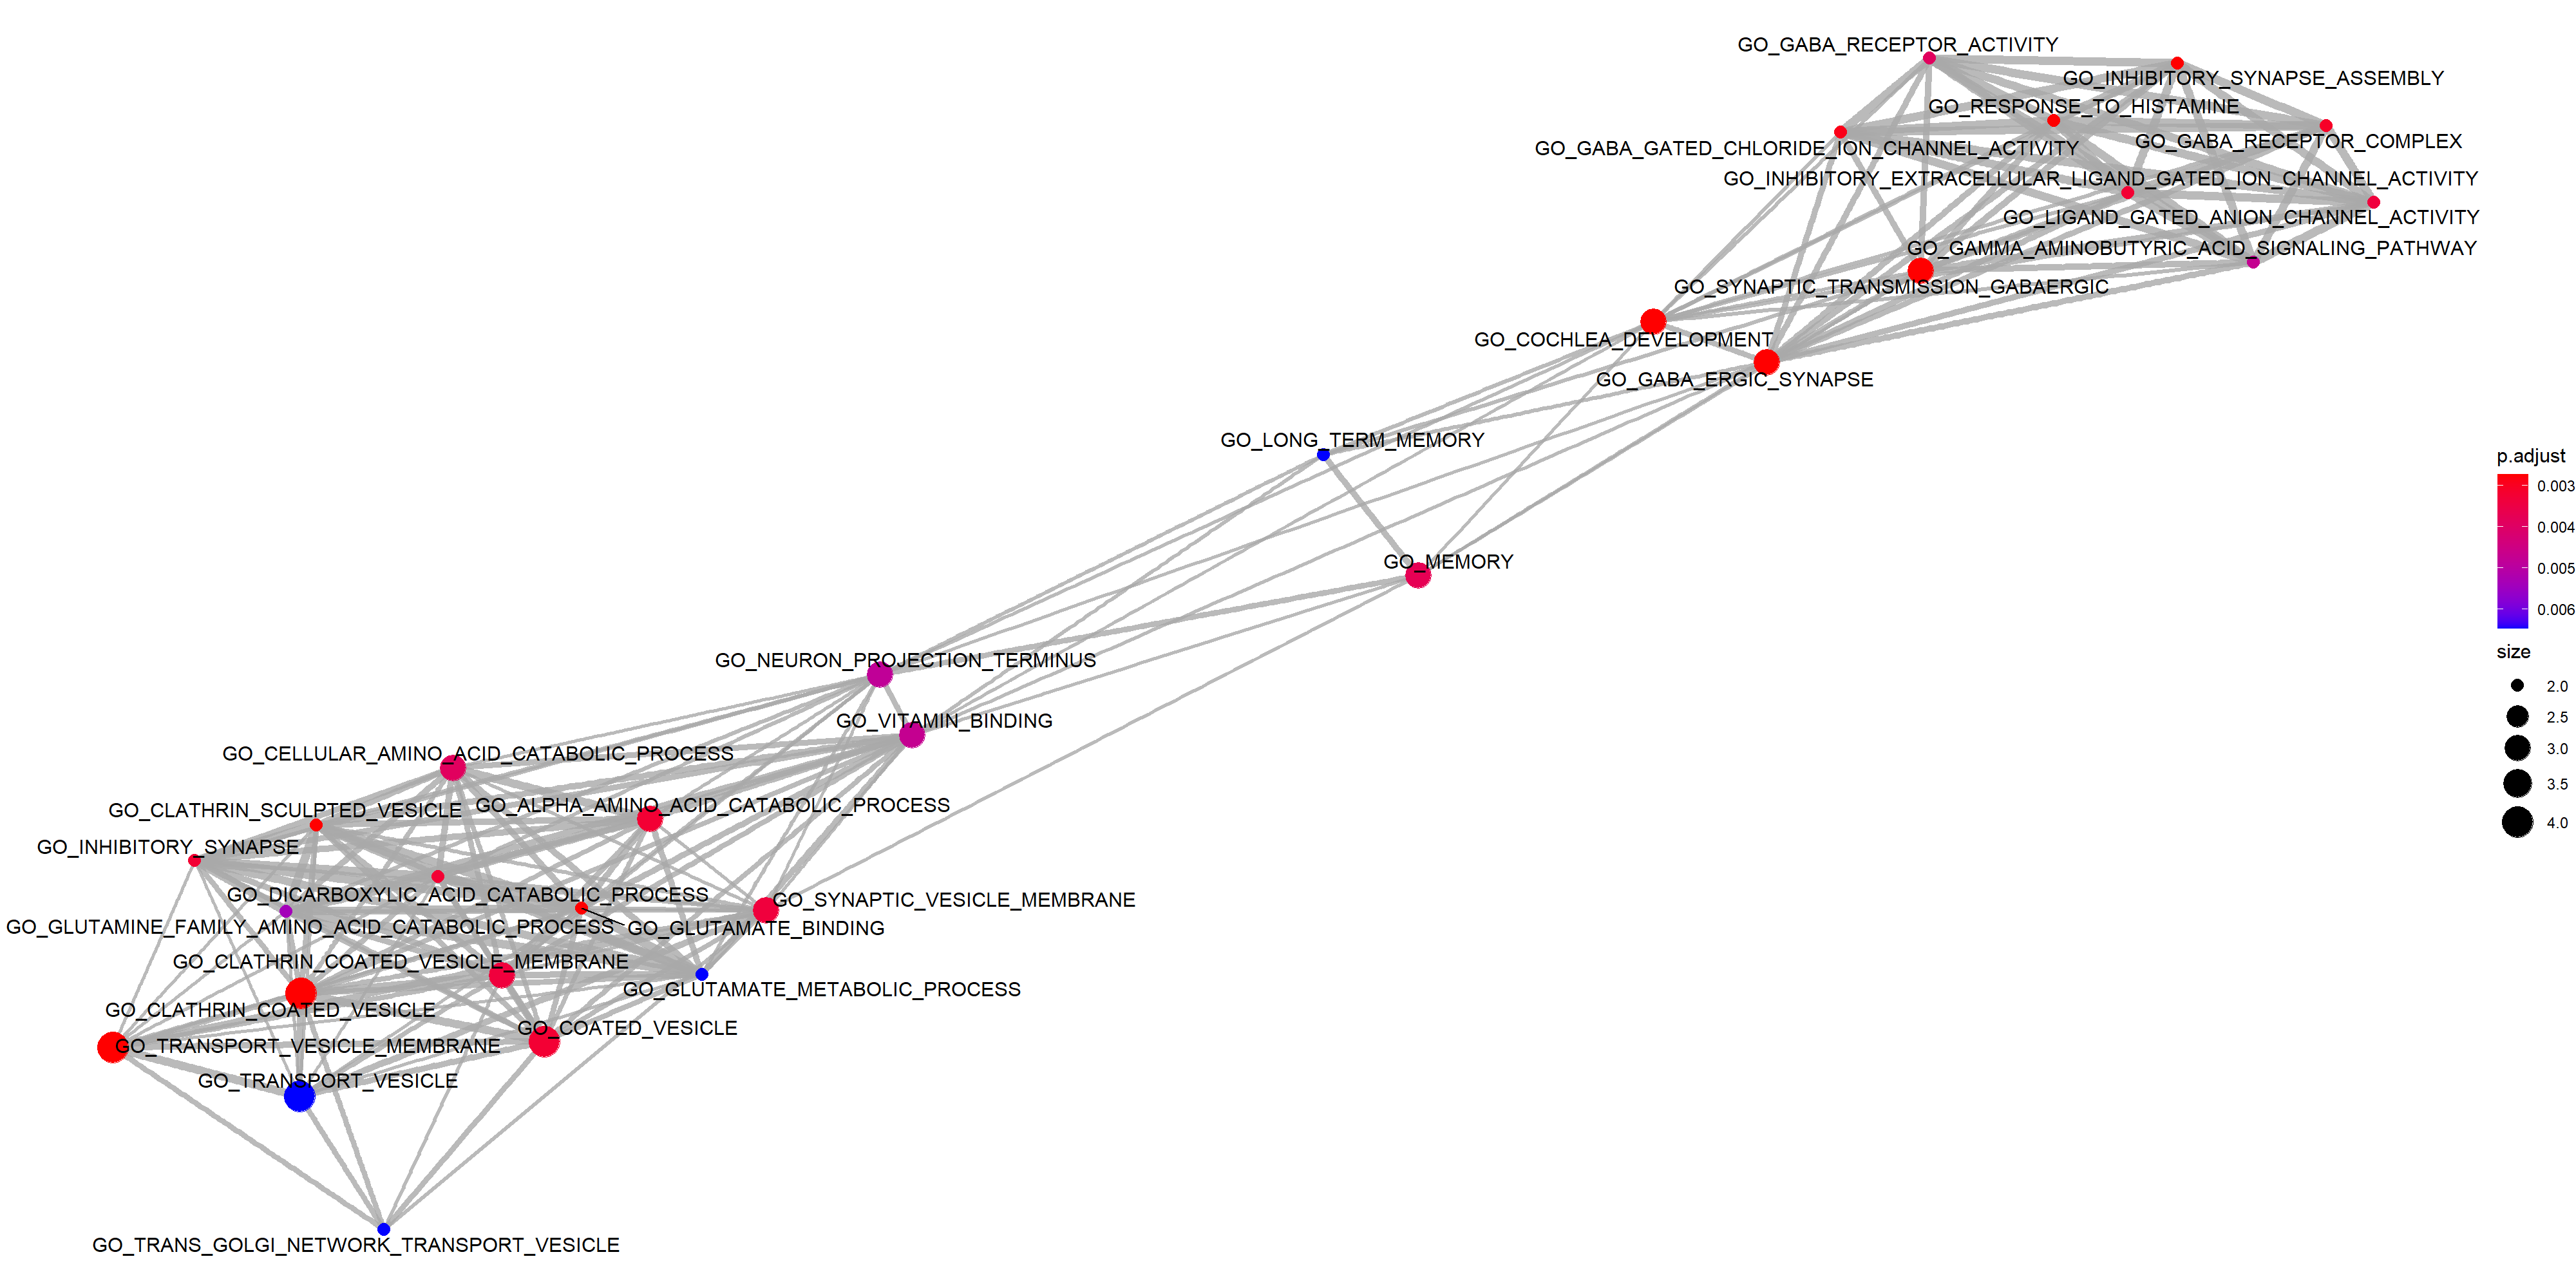
\includegraphics[width=10cm]{Figures/GSEA/CTLvsADh_ef_emapplot.png} }}%
    \\
    \subfloat[\centering Gene-concept network for ORA. ]{{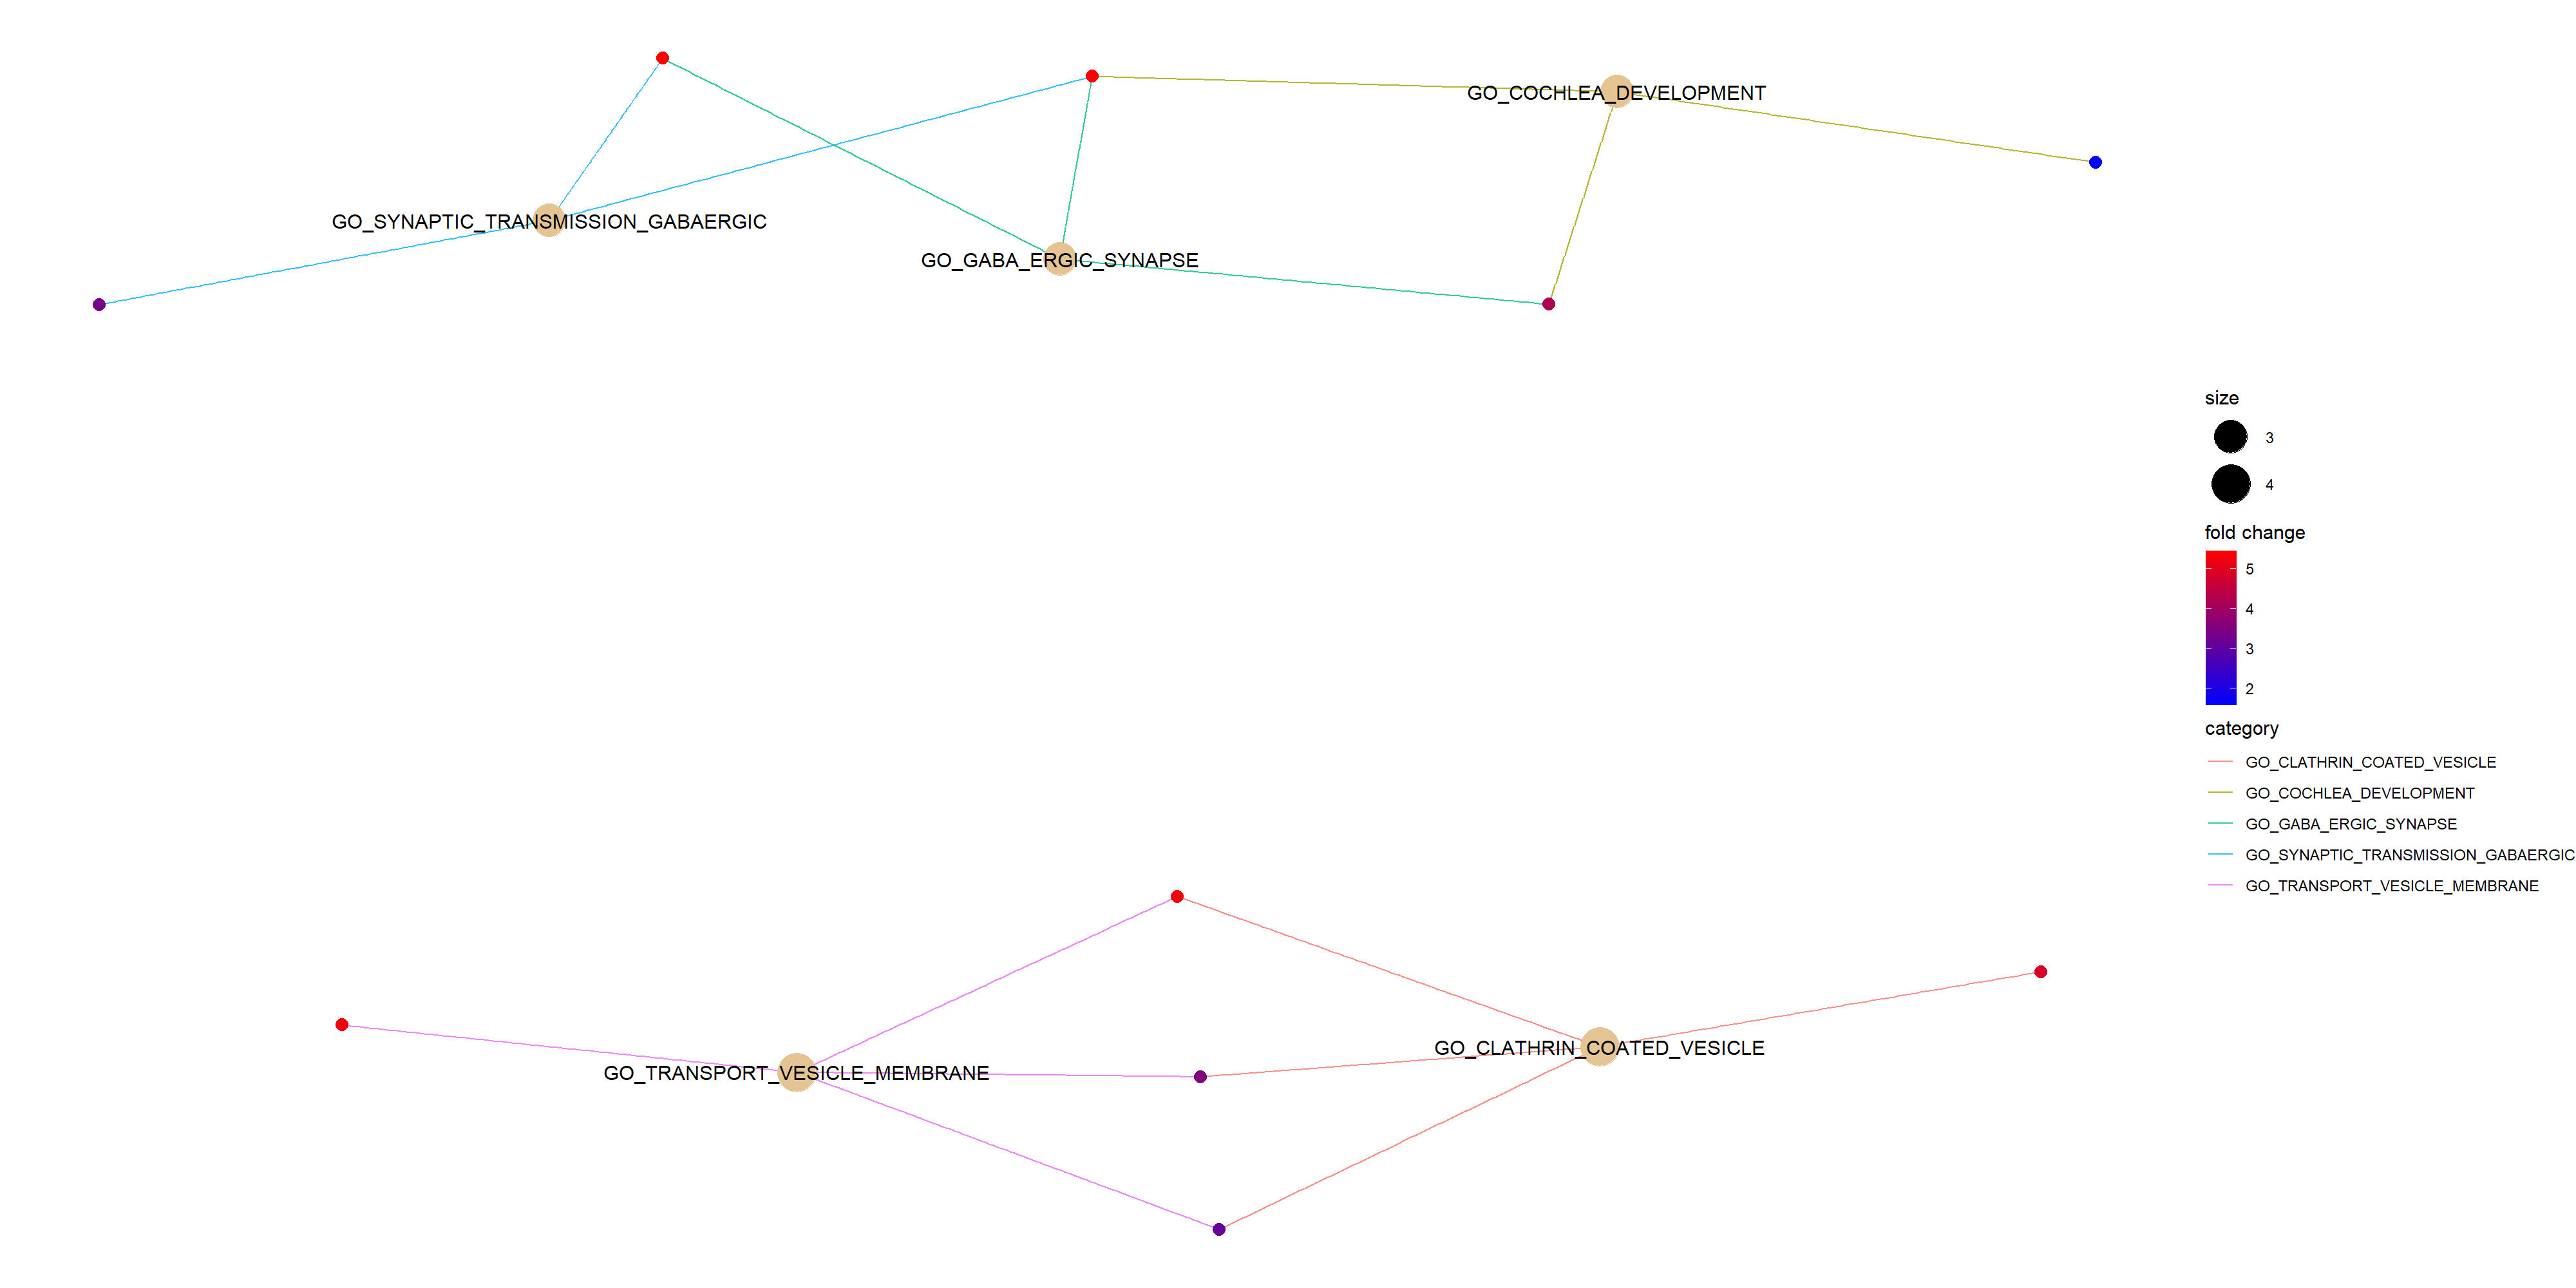
\includegraphics[width=10cm]{Figures/GSEA/CTLvsADh_ef_cnetplot.png} }}%
    \\
    \subfloat[\centering Heatmap for ORA. ]{{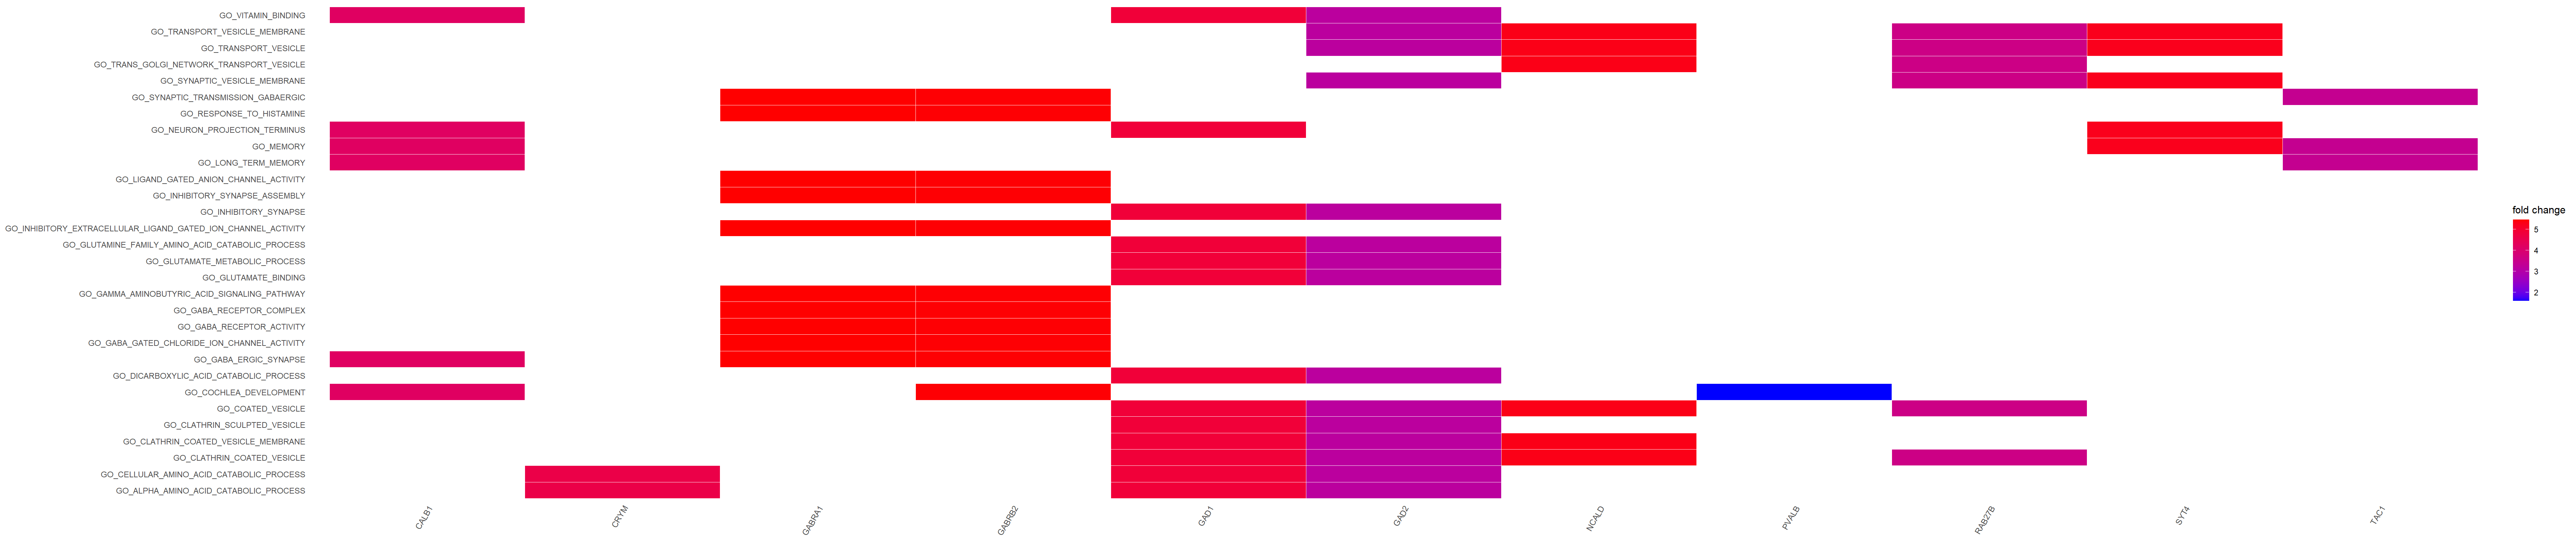
\includegraphics[width=10cm]{Figures/GSEA/CTLvsADh_ef_heatmap.png} }}%
\caption{Functional analysis visualizations of Hip-AD-f.}
\end{figure}

% AD-Hip-m
\begin{figure}[!ht]%
    \centering
    \subfloat[\centering Enrichment map for ORA. ]{{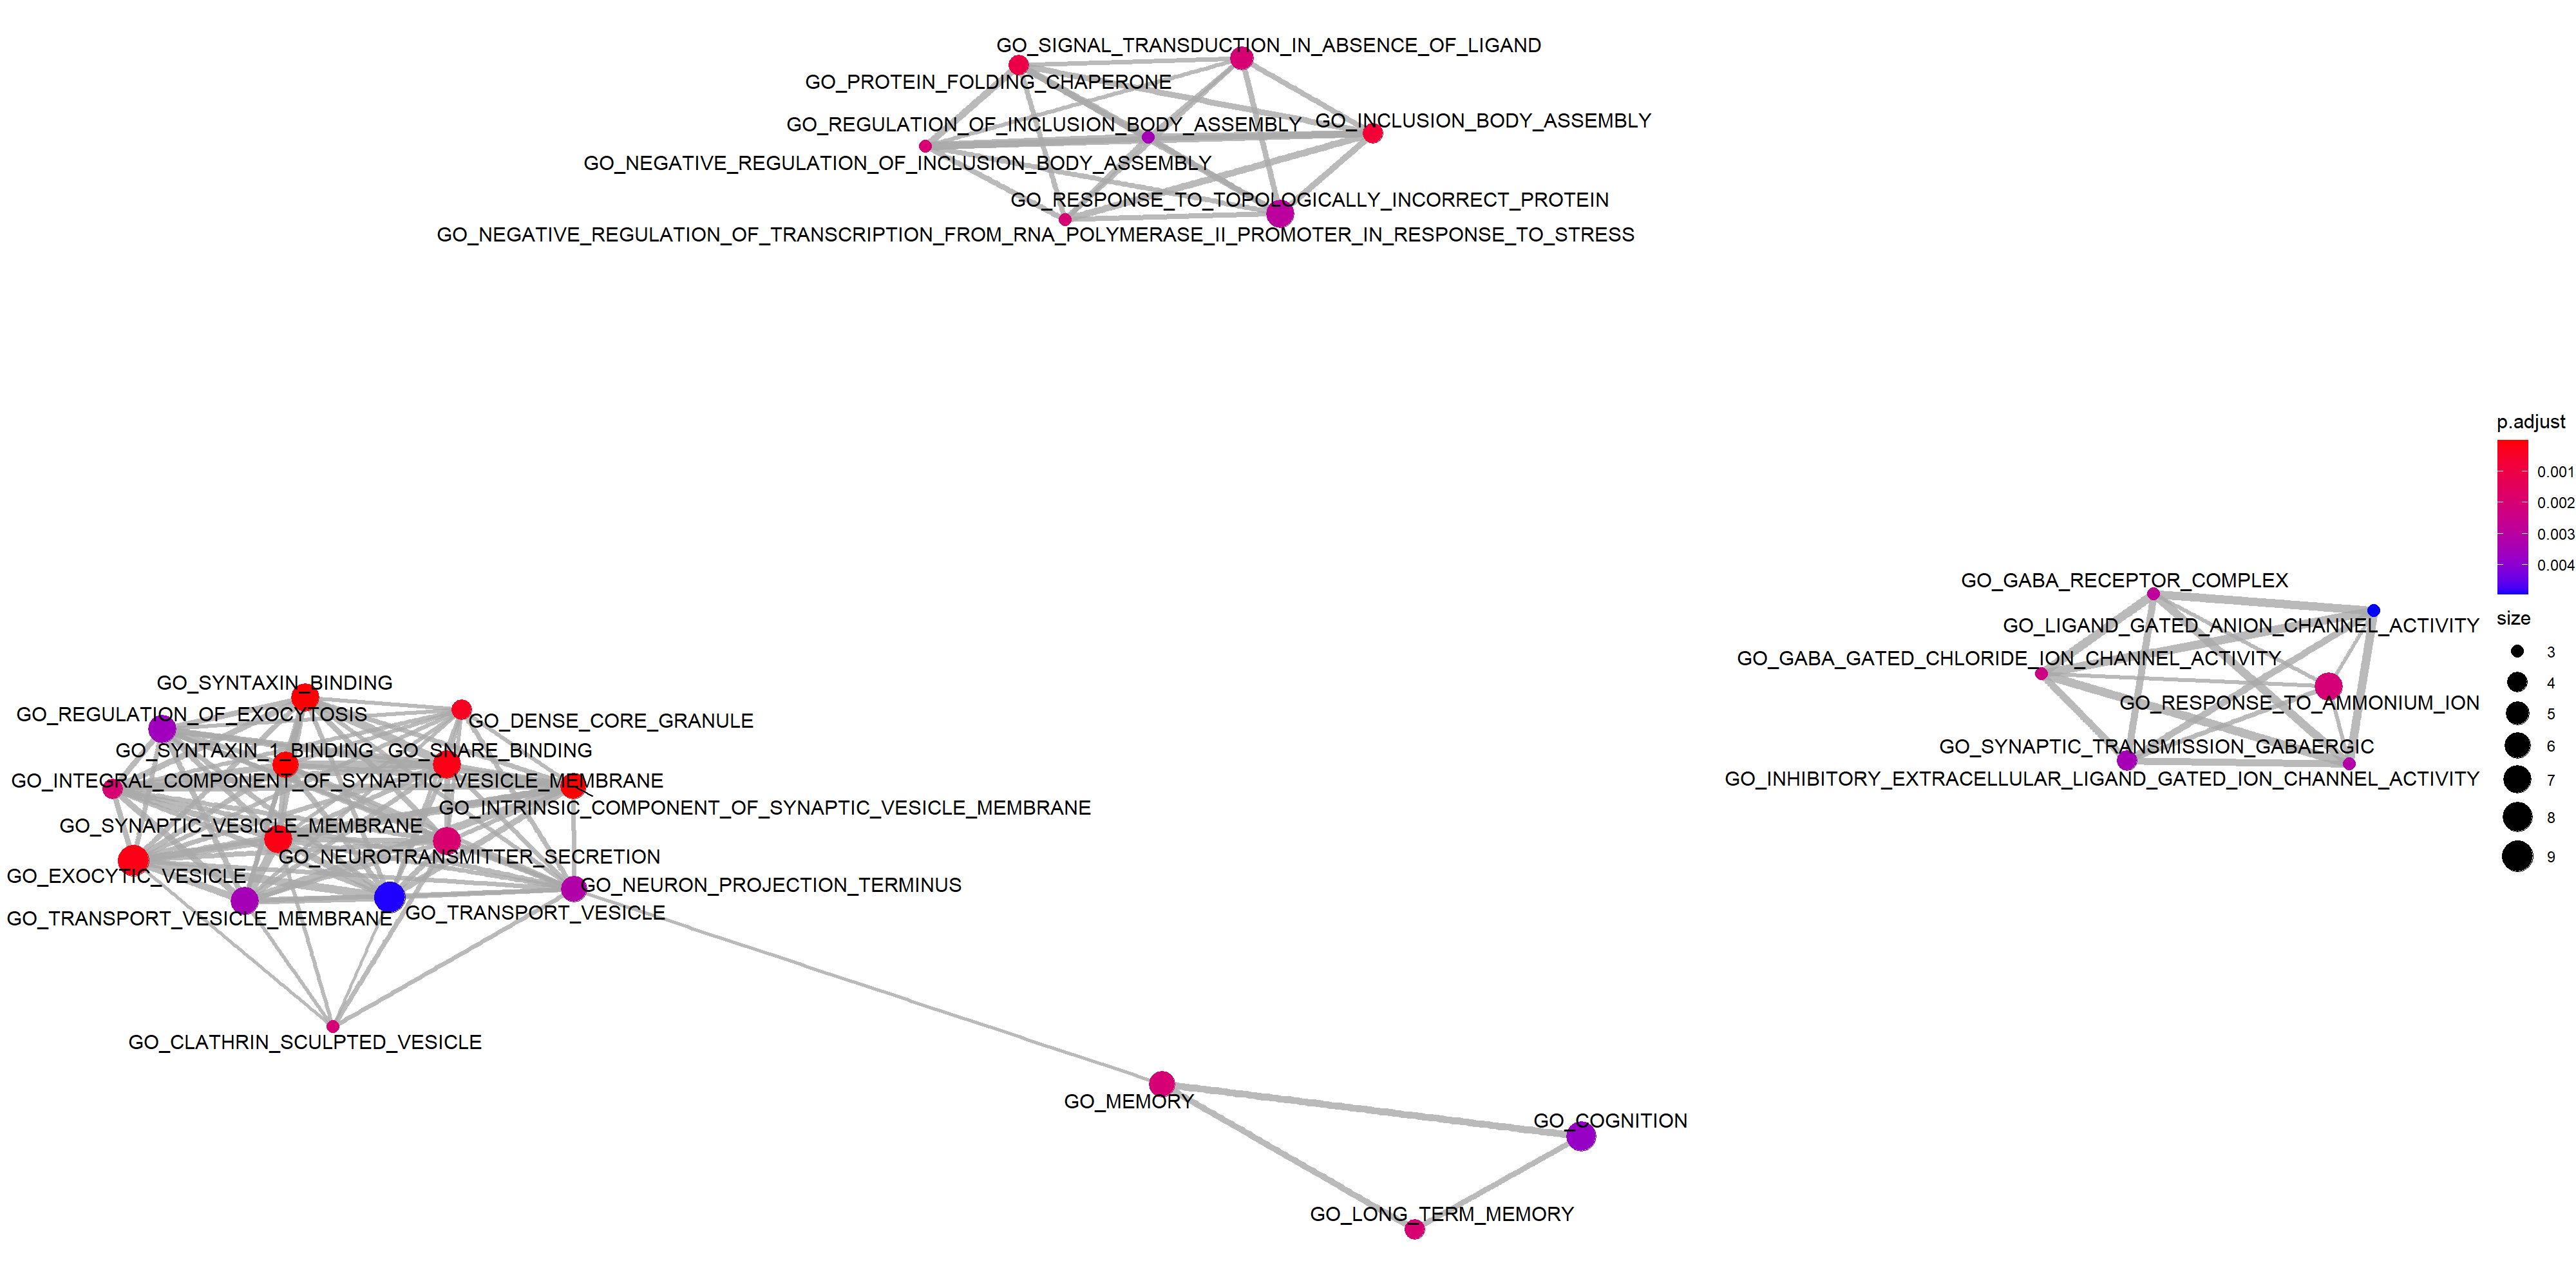
\includegraphics[width=10cm]{Figures/GSEA/CTLvsADh_em_emapplot.png} }}%
    \\
    \subfloat[\centering Gene-concept network for ORA. ]{{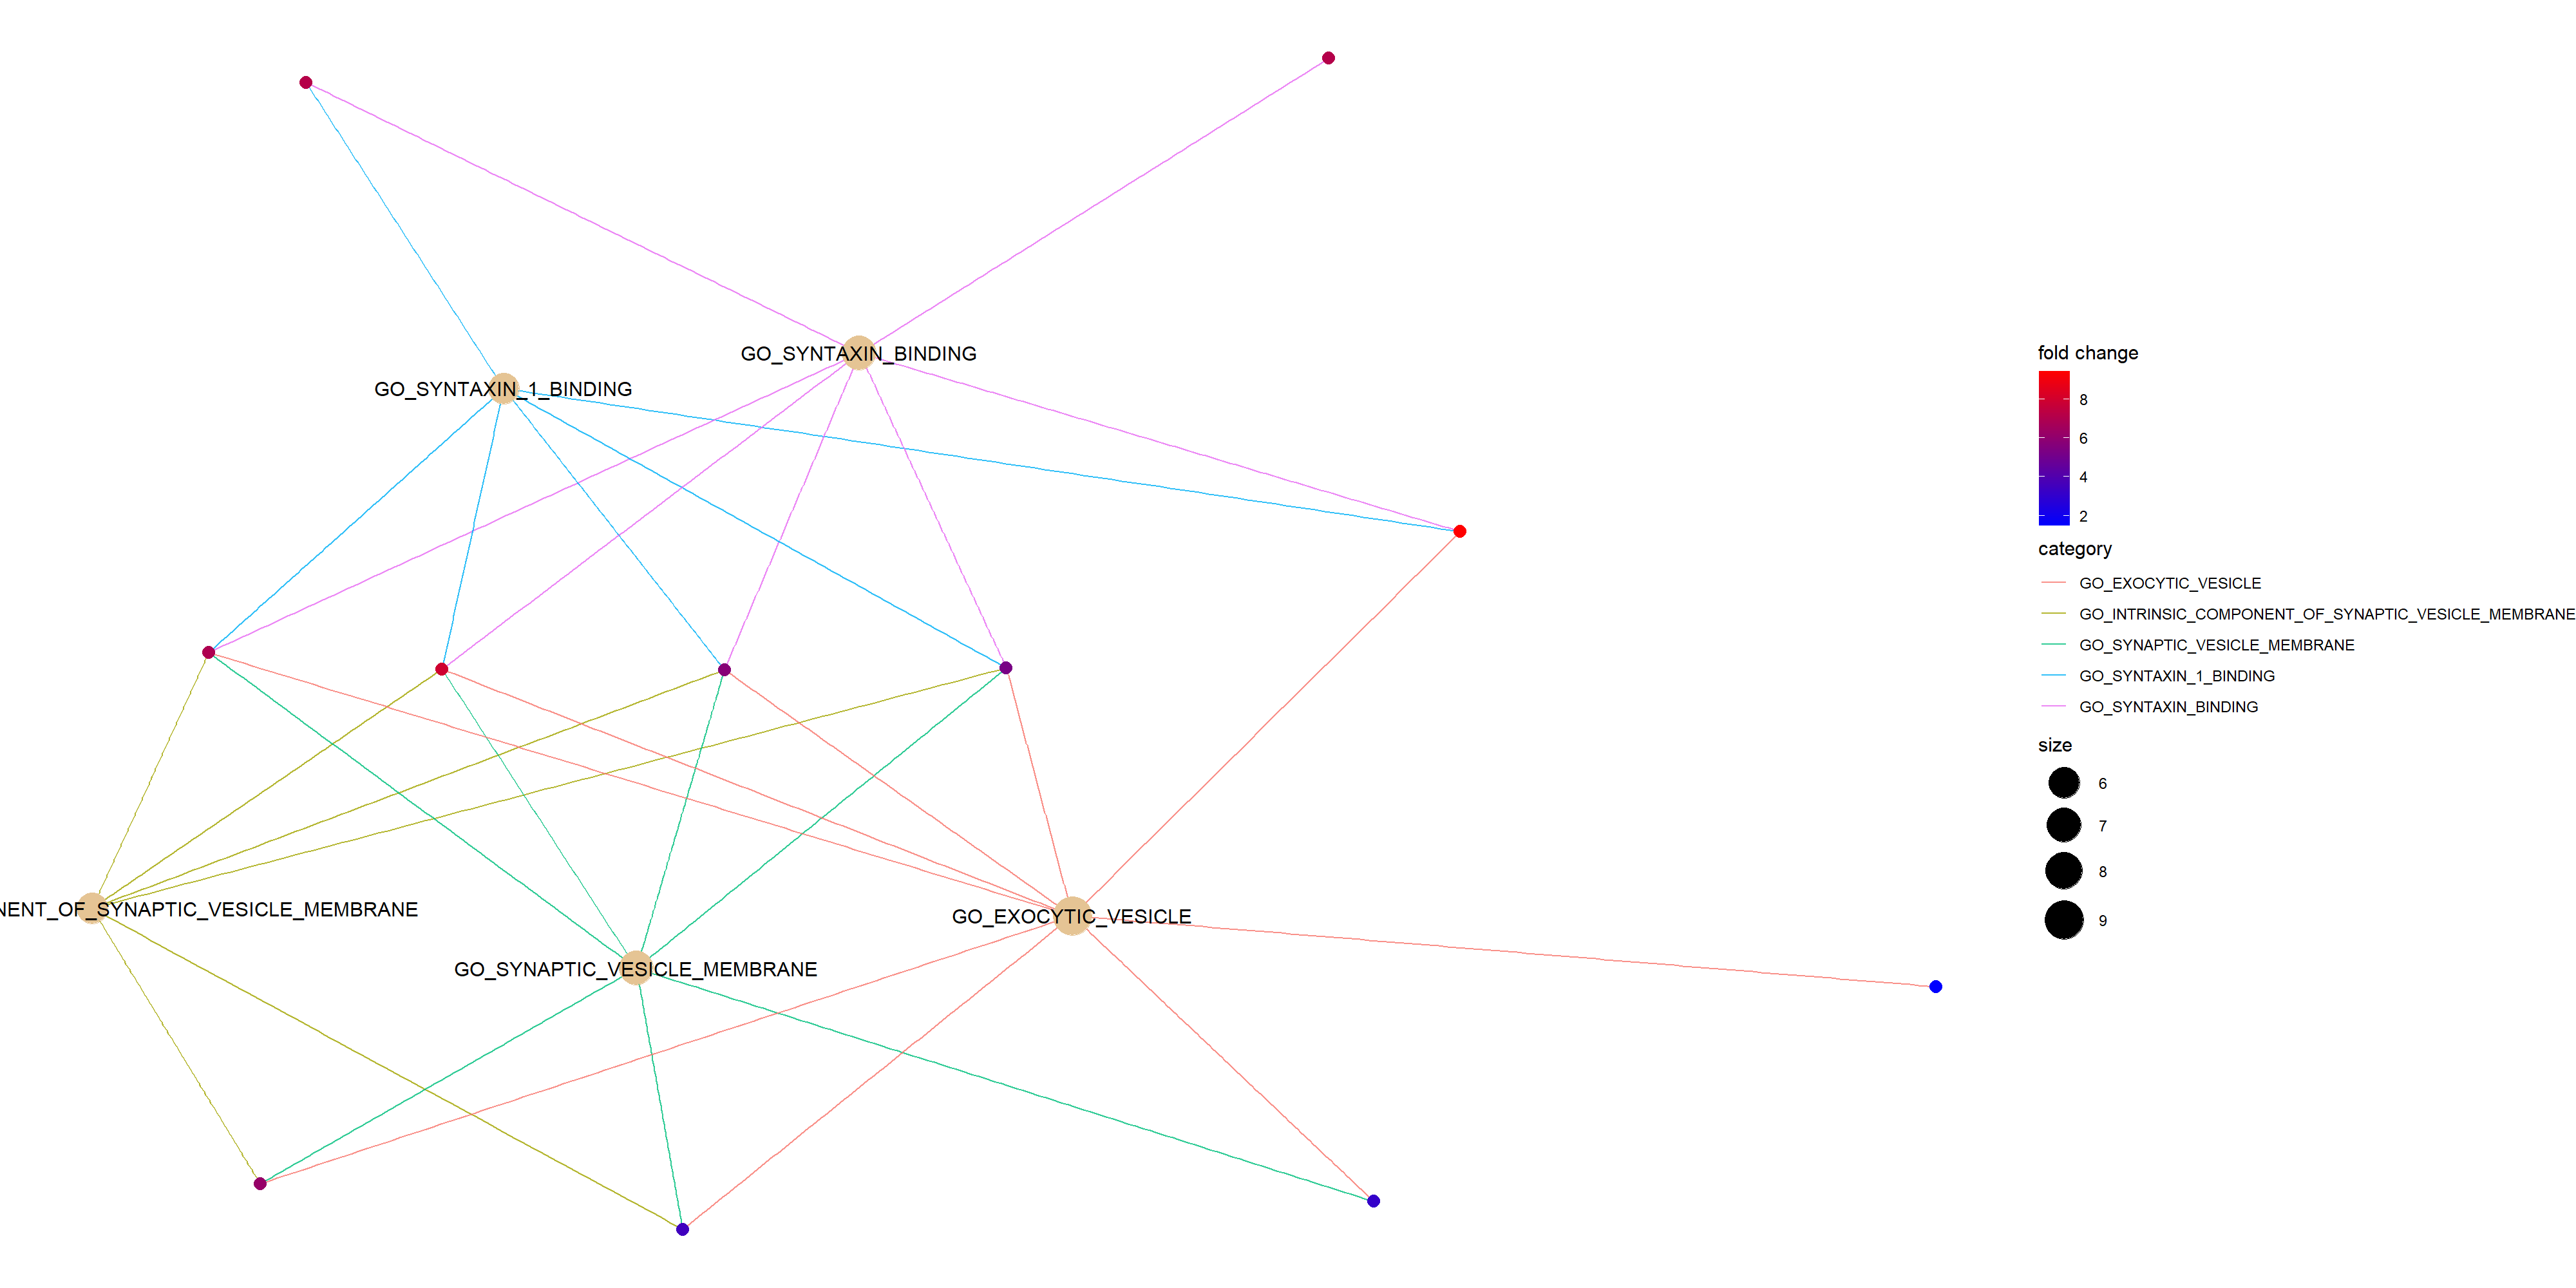
\includegraphics[width=10cm]{Figures/GSEA/CTLvsADh_em_cnetplot.png} }}%
    \\
    \subfloat[\centering Heatmap for ORA. ]{{\includegraphics[width=10cm]{Figures/GSEA/CTLvsADh_em_heatmap.png} }}%
\caption{Functional analysis visualizations of Hip-AD-m.}
\end{figure}

% AD-Front-f
\begin{figure}[!ht]%
    \centering
    \subfloat[\centering Enrichment map for ORA. ]{{\includegraphics[width=10cm]{Figures/GSEA/CTLvsADfo_ef_emapplot.png} }}%
    \\
    \subfloat[\centering Gene-concept network for ORA. ]{{\includegraphics[width=10cm]{Figures/GSEA/CTLvsADfo_ef_cnetplot.png} }}%
    \\
    \subfloat[\centering Heatmap for ORA. ]{{\includegraphics[width=10cm]{Figures/GSEA/CTLvsADfo_ef_heatmap.png} }}%
\caption{Functional analysis visualizations of Front-AD-f.}
\end{figure}

% AD-Front-m
\begin{figure}[!ht]%
    \centering
    \subfloat[\centering Enrichment map for ORA. ]{{\includegraphics[width=10cm]{Figures/GSEA/CTLvsADfo_em_emapplot.png} }}%
    \\
    \subfloat[\centering Gene-concept network for ORA. ]{{\includegraphics[width=10cm]{Figures/GSEA/CTLvsADfo_em_cnetplot.png} }}%
    \\
    \subfloat[\centering Heatmap for ORA. ]{{\includegraphics[width=10cm]{Figures/GSEA/CTLvsADfo_em_heatmap.png} }}%
\caption{Functional analysis visualizations of Front-AD-m.}
\end{figure}

% AD-Fus-f
\begin{figure}[!ht]%
    \centering
    \subfloat[\centering Enrichment map for ORA. ]{{\includegraphics[width=10cm]{Figures/GSEA/CTLvsADfu_ef_emapplot.png} }}%
    \\
    \subfloat[\centering Gene-concept network for ORA. ]{{\includegraphics[width=10cm]{Figures/GSEA/CTLvsADfu_ef_cnetplot.png} }}%
    \\
    \subfloat[\centering Heatmap for ORA. ]{{\includegraphics[width=10cm]{Figures/GSEA/CTLvsADfu_ef_heatmap.png} }}%
\caption{Functional analysis visualizations of Fus-AD-f.}
\end{figure}

% AD-Fus-f-S1
\begin{figure}[!ht]%
    \centering
    \subfloat[\centering Enrichment map for ORA. ]{{\includegraphics[width=10cm]{Figures/GSEA/CTLvs1fu_ef_emapplot.png} }}%
    \\
    \subfloat[\centering Gene-concept network for ORA. ]{{\includegraphics[width=10cm]{Figures/GSEA/CTLvs1fu_ef_cnetplot.png} }}%
    \\
    \subfloat[\centering Heatmap for ORA. ]{{\includegraphics[width=10cm]{Figures/GSEA/CTLvs1fu_ef_heatmap.png} }}%
\caption{Functional analysis visualizations of Fus-AD-f-S1.}
\end{figure}

% AD-Fus-f-S2
\begin{figure}[!ht]%
    \centering
    \subfloat[\centering Enrichment map for ORA. ]{{\includegraphics[width=10cm]{Figures/GSEA/CTLvs2fu_ef_emapplot.png} }}%
    \\
    \subfloat[\centering Gene-concept network for ORA. ]{{\includegraphics[width=10cm]{Figures/GSEA/CTLvs2fu_ef_cnetplot.png} }}%
    \\
    \subfloat[\centering Heatmap for ORA. ]{{\includegraphics[width=10cm]{Figures/GSEA/CTLvs2fu_ef_heatmap.png} }}%
\caption{Functional analysis visualizations of Fus-AD-f-S2.}
\end{figure}

% AD-Fus-f-S3
\begin{figure}[!ht]%
    \centering
    \subfloat[\centering Enrichment map for ORA. ]{{\includegraphics[width=10cm]{Figures/GSEA/CTLvs3fu_ef_emapplot.png} }}%
    \\
    \subfloat[\centering Gene-concept network for ORA. ]{{\includegraphics[width=10cm]{Figures/GSEA/CTLvs3fu_ef_cnetplot.png} }}%
    \\
    \subfloat[\centering Heatmap for ORA. ]{{\includegraphics[width=10cm]{Figures/GSEA/CTLvs3fu_ef_heatmap.png} }}%
\caption{Functional analysis visualizations of Fus-AD-f-S3.}
\end{figure}

% AD-Fus-m
\begin{figure}[!ht]%
    \centering
    \subfloat[\centering Enrichment map for ORA. ]{{\includegraphics[width=10cm]{Figures/GSEA/CTLvsADfu_em_emapplot.png} }}%
    \\
    \subfloat[\centering Gene-concept network for ORA. ]{{\includegraphics[width=10cm]{Figures/GSEA/CTLvsADfu_em_cnetplot.png} }}%
    \\
    \subfloat[\centering Heatmap for ORA. ]{{\includegraphics[width=10cm]{Figures/GSEA/CTLvsADfu_em_heatmap.png} }}%
\caption{Functional analysis visualizations of Fus-AD-m.}
\end{figure}

% AD-Fus-m-S1
\begin{figure}[!ht]%
    \centering
    \subfloat[\centering Enrichment map for ORA. ]{{\includegraphics[width=10cm]{Figures/GSEA/CTLvs1fu_em_emapplot.png} }}%
    \\
    \subfloat[\centering Gene-concept network for ORA. ]{{\includegraphics[width=10cm]{Figures/GSEA/CTLvs1fu_em_cnetplot.png} }}%
    \\
    \subfloat[\centering Heatmap for ORA. ]{{\includegraphics[width=10cm]{Figures/GSEA/CTLvs1fu_em_heatmap.png} }}%
\caption{Functional analysis visualizations of Fus-AD-m-S1.}
\end{figure}

% AD-Fus-m-S2
\begin{figure}[!ht]%
    \centering
    \subfloat[\centering Enrichment map for ORA. ]{{\includegraphics[width=10cm]{Figures/GSEA/CTLvs2fu_em_emapplot.png} }}%
    \\
    \subfloat[\centering Gene-concept network for ORA. ]{{\includegraphics[width=10cm]{Figures/GSEA/CTLvs2fu_em_cnetplot.png} }}%
    \\
    \subfloat[\centering Heatmap for ORA. ]{{\includegraphics[width=10cm]{Figures/GSEA/CTLvs2fu_em_heatmap.png} }}%
\caption{Functional analysis visualizations of Fus-AD-m-S2.}
\end{figure}